

\documentclass[11pt,letterpaper]{report}

%%  The file ``gmudissertation.sty''  is the GMU latex style file and
%%   should be placed in the same directory as your LaTeX files
\usepackage{gmudissertation}

%%
%% other packages that need to be loaded
%%
\usepackage{graphicx}                    %   for imported graphics
\usepackage{amsmath}                     %%
\usepackage{amsfonts}                    %%  for AMS mathematics
\usepackage{amssymb}                     %%
\usepackage{amsthm}                      %%
\usepackage{epstopdf}                    %   for postscript files
\usepackage[normalem]{ulem}              %   a nice standard underline package
\usepackage{setspace}                    %   for line spacing commands
%\usepackage[noadjust,verbose,sort]{cite} %   arranges reference citations neatly
%\usepackage{booktabs}
%\usepackage{subfig}
%%\usepackage{tabularx}
%%\usepackage{sidecap}
%\usepackage{rotating}
%\usepackage{wrapfig}
%\usepackage{dcolumn}
\usepackage{float}
%\usepackage[section]{placeins}
%\usepackage[backref=false,breaklinks,bookmarks,colorlinks=false,citecolor=black]{hyperref}
\usepackage{multirow}
%%\usepackage{mathrsfs}
%\usepackage{calrsfs}
\usepackage{graphicx}
\usepackage{amsfonts}
\usepackage{amssymb}
\usepackage{amsmath}
\usepackage{mathrsfs}
\usepackage{braket}
\usepackage{epstopdf}
\usepackage{pdfpages}
% \usepackage{geometry}

\def\avg#1{\langle#1\rangle}
\def\v#1{\mathbf{#1}}
\def\Re {\mbox{Re}}
\def\Im {\mbox{Im}}
\def\tr{\mbox{tr}}
\def\nn{\nonumber}
\def\pp{\parallel}
\def\ket#1{\vert #1 \rangle}
\def\bra#1{\langle #1 \vert}
\def\me#1#2#3{\langle #1 \vert #2 \vert #3 \rangle}
\def\Br{\mathbf{r}}

\newcommand{\kp}{k_{+}}
\newcommand{\ki}{k_{-}}
\newcommand{\idz}{i\partial_z}
\newcommand{\kperp}{\mathbf{k}_\parallel}

%% The file ``mydissertationabbrev.sty'' is an (optional) personalized file that
%% may contain any and all LaTeX command (re)definitions that will be used
%% throughout the document
%\usepackage{mydissertationabbrev}

\addtolength{\intextsep}{3cm}
\addtolength{\textfloatsep}{3cm}

\beforedoc

\begin{document}

%% In this section, all of the user-specific fields to be used in the
%% title pages are set
\title{Heterostructures of Topological Insulators and Superconductors}
\onelinetitle{Heterostructures of Topological Insulators and Superconductors}
\author{Mahmoud Lababidi}
\degree{Doctor of Philosophy}
\doctype{Dissertation}
\dept{Physics, Astronomy and Computational Science}
\discipline{Physics}

% \seconddeg{.}
% \seconddegschool{.}
% \seconddegyear{.}

\firstdeg{Bachelor of Science}
\firstdegschool{University of Florida}
\firstdegyear{2006}

\degreeyear{2013}

% Note: semester name should be written in its full-form. For example, Fall Semester, not just Fall.
\degreesemester{Summer Semester}

\advisor{Dr. Erhai Zhao}
\firstmember{Dr. Dimitrios A. Papaconstantopoulos}
\secondmember{Dr. Predrag Nikolic}
\thirdmember{Dr. Qiliang Li}
\depthead{Dr. Michael E. Summers}
\adeanCOS{Dr. Timothy L. Born}
\deanCOS{Dr. Vikas Chandhoke}

\signaturepage
%\signaturepagex

\titlepage
\copyrightpage

\dedicationpage
\noindent \begin{center} To Angus Macgyver, who needed only a roll of duct tape,\\ paperclip, and a Swiss Army knife to solve any problem. \\
To my parents, Lina and Steve, for sacrificing their lives\\ for me, my future, and my success and happiness in life.% To the rest of my family and my friends for their continual support. 
\end{center}



\acknowledgementspage 
\noindent First and foremost, I'd like to thank the most driven, understanding and supportive advisor anyone could ask for, Erhai Zhao. Not only have I learned more about physics than I could ever imagine, he has mentored me on being a good scientist, and a disciplined worker. I really could not have asked for a better advisor to lead me through this fascinating journey.
I'd like to thank Dr. Papa for his incredible generosity from day one. He supported me throughout my PhD and without that support I would not have successfully completed the many projects and publications I have had. 
I consider Paul So to be more than just a graduate department advisor. You could add resident psychologist to his title and it would be wholly appropriate. Without his clear guidance on all topics, including ones beyond physics and art, I would be a lost soul. 
Furthermore, I thank Mike Summers for his help as a department chair and helping me in times of need. He has supported me financially at times and has always had an open door for me and any graduate student to talk to him.

Joe Weingartner would be considered the ``House Dad'' of the fraternity of the physics department. He has been a guiding light to me in many ways including physics and life. He is without a doubt one of the most important people the department has given tenure to for his kindness and empathy for anyone who walks into his office.
I am very grateful to Indu Satija for her amazing creativity and beautiful ability to see physics like no one has. I give her full credit for the idea that spawned my most fascinating project on the driven quantum Hall system. 
I thank Predrag Nikolic, not only as helpful committee member but as great educator. He has always welcomed healthy discussion about a variety of topics that have helped me in my career numerous times.
Qiliang Li has been one of the most excited and appreciative members I could have on my committee. His enthusiasm towards my work has been a heavy driver for a significant portion of my research.
Ming Tian was the first person to take me in under her wing as a student. She saw I had potential and ability to do physics and immediately gave me challenging problems to work on. She has been very supportive of my endeavours even if it meant changing groups.
I thank Gerald Cook, the first Professor I interacted with during my first steps inching towards the wormhole of grad school, and his early enthusiasm for me to begin this journey.
Phil Rubin was the person that urged me to apply to the program regardless of my physics background because he believed I'd do great. Somehow he was right. I later learned Phil was in a Psychology PhD program when he switched to physics. That's serious inspiration.

Without Kathleen Enos, Mari-Elaine Triolo, Geoff Elkins, Stephanie Monk, and Melissa Hayes I would be wrapped up in more paperwork than I could handle. They have made my this trip as smooth as possible and have been the best people to have around.
Of course without Dan Thomas and Andrew Abdalian I'd be a headless chicken running around with regards to my IT issues.


Thank you Stephen Gildea for inspiring me to go to graduate school by becoming a rocket scientist and kicking ass at it.
Anish Mitra, my first friend in graduate school and roommate, deserves much recognition for being the one person that was as interested in math and science as I was. 
Indrajit Das and Zrinka Greguric Ferencek are staples in my early career. I owe much to them for their stimulating discussions while we completed course work together. 
Timofey Frolov is my favorite Russian physicist, metal guitarist, food snob I've ever known. He has been a great friend and colleague during our years at GMU before he ditched me for Berkeley. 
Ol' Dirty himself, Greg Byrne, deserves more than a mention here for our antics during these years especially at the Arlington Office.
Many thanks go to Devin Vega and our enjoyable and stimulating discussions in course work and research under Ming Tian.

Quite importantly, I'd like to thank Lois Cohen, Edmund Lau, and Jean Wright for their influence during my formative high school years.  I owe them more than just a line in this theses and without them I truly would not be here. The same goes for Anand Rangarajan and Eric Schwartz from my time at University of Florida, two professors who challenged me in innovative and creative ways.

Not least, I'd like to thank SPACS, Office of Naval Research, Air Force Office of Scientific Research, National Science Foundation and National Institute of Standards and Technology for the funding they have provided me over these years.


%%
%% Table of contents, list of tables, and lists of figures
%%

\tableofcontents

%\listoftables

\listoffigures

\chapt{List of Symbols}
%%\addcontentsline{toc}{chapter}{List of Symbols}
\begin{tabbing}
  aaaaaaaaaaaaaa\=\kill
  $v_F$\>Fermi velocity of Dirac electrons\\
  $\vec{k}$\>momentum vector\\
  $k_i$\>momentum in the $i$-th direction\\
  $\mathcal{E}_F$\>Fermi energy\\
  $A(x,k,\epsilon)$\>spin($\sigma$), momentum and position resolved density of (energy) states\\
  $N(x,\epsilon)$\>spin($\sigma$) and position resolved density of (energy) states\\
  $\mu$\>chemical potenial, sometimes as Fermi energy ($\mathcal{E}_F$)\\
  $\mathcal{H}$\>Hamiltonian\\
  $\psi(x)$\>wave function of particle\\
  $u_\sigma$ ($v_\sigma$)\>Bogoliubov-de Gennes quasi-particle (hole) wave function\\
  $k_B$\>Boltzmann's constant\\
\end{tabbing}

%%
%% Abstract
%%
\abstractpage
Topological insulators (TI), such as Bi$_2$Se$_3$, 
are a new class of quantum materials discovered recently. They are insulating in the bulk but
can conduct on the surfaces. The robust surface states of three-dimensional strong TIs form a unique two-dimensional system of massless electrons, known as a helical metal, with a linear energy-momentum dispersion and spin-momentum locking. While these surface modes alone have spurred great interest, their interaction with superconductors (S) in close proximity has opened up opportunities to engineer topological superconductivity using TI-S heterostructures. This thesis is a microscopic, self-consistent theoretical investigation of the interplay between TI and superconductors. Three types of TI-based heterostructures with increasing complexity are studied in detail. 

We first present a detailed study of the coupling between a metal and a topological insulator. We compute the spin-active scattering matrix for electrons coming from the metal incident on the metal-TI interface. We find that there exists a critical incident angle, where perfect spin-flip occurs as the incoming electron is reflected. We discuss the origin of this phenomena and its potential implications in spintronics. We then compute the local spectrum at the metal-TI interface, and examine its evolution from the tunneling limit (bad contact) to the strong coupling limit (good contact). The calculations are done using two complementary approaches; in a continuum model based on a k$\cdot$p Hamiltonian a wave function matching approach is taken and the lattice model requires the use of lattice Green's functions. The study of metal-TI interface lays the foundation for our subsequent theory of S-TI interface.

Next we carry out microscopic, self-consistent calculations of the superconducting order parameter and pairing correlations near a S-TI interface, where S is an $s$-wave superconductor. We discuss the suppression of the order parameter by the topological insulator and show that triplet pairing correlations are induced by spin-flip scattering at the interface. We verify that the interface spectrum at sub-gap energies is well described by the Fu-Kane model even for strongly coupled S and TI. These sub-gap modes are interface states with spectral weight penetrating well into the superconductor. We extract the phenomenological parameters of the phenomenological Fu-Kane model from our microscopic calculations, and find they are strongly renormalized from the bulk material parameters. 
\thispagestyle{empty}

Building upon such understanding of single TI-S interface, we move on to examine a TI surface in contact with two superconductors with a phase bias, namely a Josephson junction patterned on the TI surface and mediated by the helical metal. A short Josephson junction of this kind at a phase bias of $\pi$ is known to give rise to exotic quasiparticle excitations known as Majorana fermions with a linear dispersion, $E\sim k$. Our self-consistent calculation of the 
Andreev bound states spectrum reveals, for the first time, a new regime with very different physics in these devices. 
We show that the subgap spectrum becomes nearly flat at zero energy when the chemical potential is sufficiently away from the Dirac point. The flat dispersion is well approximated by $E\sim k^N$, where $N$ scales with the chemical potential. We find a similar linear-to-flat dispersion evolution also occurs for the subgap spectrum of a periodic superconducting proximity structure, such as a TI surface in contact with a striped superconductor.

The systematic microscopic study of TI-S heterostructures helps interpret the data from ongoing experiments on these structures. The formalism developed also forms the basis for subsequent investigation of more complicated layered materials such as the periodic array of magnetically doped TI and S which is argued to give rise to an exotic topological superconductor known as Weyl superconductor.

\thispagestyle{empty}
%% Be sure to leave a line of whitespace immediately before this line!!!!!
%% (If this comment segment runs together with the preceding text, you might
%%  see the second page of the abstract numbered "0".)
%%
%% If the abstract is more than one page, then place this line PRECISELY
%% at the page break; otherwise, comment it out.  (See note about this line
%% in the usage notes.)
%% \abstractmultiplepage \noindent 


%%
%%  the main body of the dissertation
%%

\startofchapters


\chapter{Introduction}

This thesis presents a systematic theoretical study of the interaction and interplay between a new class of materials named Topological Insulators (TIs) and superconductors. It consists of five chapters. The first chapter contains a brief introduction to TIs and superconductors. In addition, it describes basic concepts and notations used later in the bulk of the thesis. These include the topological surface states of a TI, the spin texture of the TI surface, phenomenological description of a superconductor coupled to a TI, exotic superconductors, and a Josephson junction structure on a TI surface. The second chapter presents a study of the interaction between metal and TI, and electron scattering at the M-TI interface. This chapter provides insight into understanding the effect of spin-orbit interactions on incoming arbitrarily spin-polarized electrons. The third chapter is a microscopic study of a heterostructure of a superconductor with a TI. The motivation is to understand the effect of a TI on an $s-$wave superconductor. The fourth chapter examines Josephson junctions on a TI surface and delves into new aspects of the energy spectra in regimes not studied before. 
%
%The fourth chapter describes an investigation on the newly proposed scheme to engineer a gapless Weyl superconductor through layering of superconductors and TI. Each of the chapters has an introduction section that outlines how the focused study plays a role in the larger scheme of the thesis. It will also give an overview of the chapter and what parts have been published. 
Each chapter beyond Chapter 1 represents an original work published in Physical Review B. 

\section{Topological Insulators}
The field of condensed matter physics has a history of understanding phases of matter that have been condensed. Where the early focus was on solids and liquids, the field has transitioned into studying a rich variety of novel phases that are much more complex. A result of the exploration of many of these novel phases, the concept of order arose, allowing, not only the ability to categorize these phases by recognizing the type of order the system had but the order is usually associated with symmetries of the system. This idea is clearly seen in the phase transition of liquid atoms with rotational and translational symmetry into a crystal with discrete symmetries (e.g. translational, discrete rotational, inversion, etc.). An extension to this would be a paramagnet transitioning into a ferromagnet, thus breaking time-reversal symmetry. While this study of symmetry breaking is at the heart of condensed matter and allows for a deeper understanding, it is not the full story. 

In 1980 Klaus von Klitzing et al performed an experiment measuring the Hall conductance of semiconductor heterostructures in a strong magnetic field\cite{klitzing_new_1980}. What they found in the experiment was that the measured Hall conductance came in exact quantized fundamental units of $e^2/h$,
\begin{equation}
\sigma = \nu \frac{e^2}{h},
\end{equation} 
where $\nu$ is an integer value. 
The significance of this result was not only in the quantized nature of the Hall conductance, but something a bit deeper. This integer quantum Hall effect was special because this result could not be described through the usual symmetry breaking language. In the heterostructure used in the experiment, the internal ``bulk" of the system is effectively a two dimensional electron gas exposed to a strong magnetic field. The strong magnetic field puts the electrons in a cyclotron orbit and forces the electrons into discrete energy levels, the Landau levels. This effect is rather similar to a harmonic oscillator where an electron is in a spatially quadratic electric potential well ($V(x)\propto x^2$). These separated energy levels allows for the system to be an insulator when the Fermi energy is placed within the gap between two separate energy levels. While this system is in an insulating state,the edge is still a host to electronic states that propagate in a chiral manner. This discrepancy between the ability to describe bulk of the material and its edge is the issue at hand. 

The quantum Hall effect (QHE) is actually a topological phase of matter, with its energy bands described by topological invariants known as Chern numbers.
%, meaning it has topological order. Systems with topological order have long-range entanglement and a ground state degeneracy that cannot be lifted by any local perturbation. 
An integer QH phase protected from being deformed into a phase with different topology in the same way a donut (torus) is protected from being deformed into a sphere. The only time such a change is possible is through a phase transition where the gap in the energy spectrum closes in a critical fashion. 
More discussions on topological phases of matter can be found in literature.
%Many discussions on topological order can be found in many literature and any continued discussion about topological order in farther depth would not be appropriate, for this thesis does not represent any study of topological order in this form. 

\begin{figure}
\center
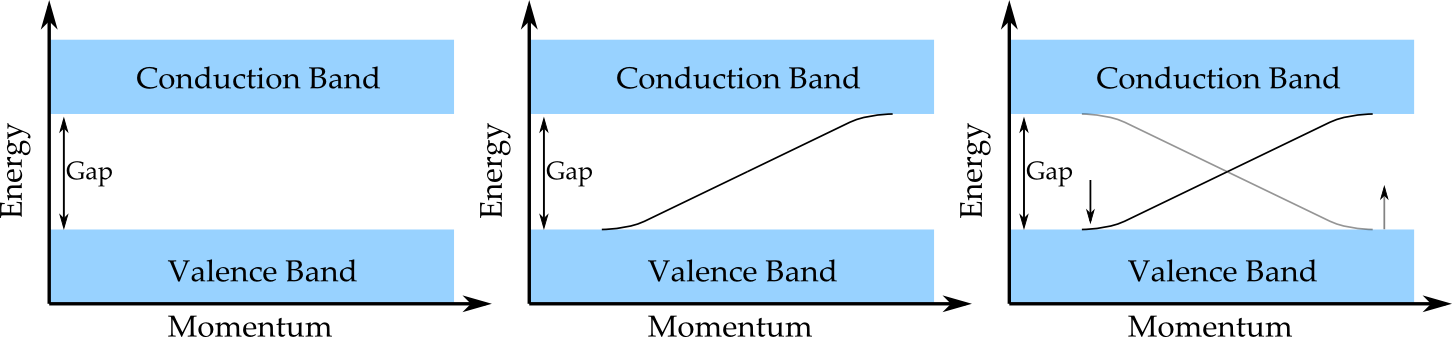
\includegraphics[width=\textwidth]{include/bands2.png}
\caption{(a) Energy spectrum of a trivial band insulator where two bands, conduction and valence, are separated by an energy gap. 
(b)  Energy spectrum of a quantum Hall state. The gap now has one chiral edge state connecting the valence band to the conduction band.  
(c)  Energy spectrum of a 2D TI (QSH). The gap now has one pair of chiral edge states connecting the valence band to the conduction band.  One line is for the spin up state and the other is for the spin down state. This essentially mimics two copies of the quantum Hall state for each spin.
}\label{insulators}
\end{figure}

We use the QHE as a lead-in for the topological insulator. 
%Though the topological insulator is a slight misnomer because of the lack of topological order (i.e. long-range entanglement), we will shortly see where the topology plays a role in it. 
By taking the QHE, we can extend it in the following way. The QHE is a gapped system with chiral edge states that depend on the applied magnetic field (see Fig. \ref{insulators}). The chirality of the edge states depend on the direction of the magnetic field, i.e. positive (negative) chiral motion of the electrons for positive (negative) out of plane magnetic field. If a system were to have both positive and negative magnetic fields simultaneously for two different species of electrons, we would see the electrons follow the two chiral motions simultaneously depending on their species. The two different species of electrons are, of course, spin-up and spin-down electrons which couple to the two magnetic fields. This system is a prototype of the quantum spin Hall effect. Kane and Mele first proposed the QSH to exist in graphene with spin-orbit coupling \cite{kane_quantum_2005}. Shortly afterwards, Bernevig, Hughes, and Zhang proposed a realistic experimental setup to host the QSH effect \cite{bernevig_quantum_2006}. Their proposal, which was verified successfully in an experiment by Koenig's group \cite{konig_quantum_2007}, exploited the spin-orbit coupling and band inversion in a HgTe-CdTe-HgTe heterostructure to create pairs of counter-propogating edge states, which are related to each other by time reversal symmetry. The QSH insulator is a 2D topological insulator. An effective Hamiltonian for the edge state can be written as 
\begin{equation}
H=\hbar v_F \sigma_x k_y,
\end{equation}
where the basis is for spin up and spin down and the resulting eigen energies are $E=\pm \hbar v_F k_y$. $v_F$ is the Fermi velocity. This is a massless Dirac Hamiltonian and the spectrum forms a Dirac crossing. 
 
The existence of a surface state can be seen in the following manner. If a topological insulator has a parameter that can be tuned to transition from topologically non-trivial to trivial, the gap of the insulator must close. When a TI is interfaced with a trivial insulator, such as the vacuum, the parameter effectively causes the gap to close at the interface, which gives rise to the gapless surface state.

In principle, by stacking sheets of the 2D TIs and forming a 3D structure, this would be a ``weak" topological insulator. The other extension of the TI from 2D to 3D  is a ``strong" topological insulator. Here, there is also an insulating 3D bulk and the 2D surfaces interfacing the vacuum are similar to the edge state of the 2D TI in their linear dispersing behavior, but they allow momentum to be in any in-plane direction, $\vec{k}=(k_x,k_y)=(k \cos(\theta),k \sin(\theta))$. The effective low-energy Hamiltonian for these surface states is
\begin{equation}
H=\hbar v_F (\sigma_x k_y - \sigma_y k_x).
\end{equation}
The energies and their respective eigenvectors
\begin{equation}
E=\pm \hbar v_F |\vec{k}|\quad
\ket{\psi_{\bf{k}}}=\frac{1}{\sqrt{2}}\left(\pm i e^{-i \theta}\ket{\uparrow}+\ket{\downarrow}\right)
\end{equation}
 where $|\vec{k}|=\sqrt{k_x^2+k_y^2}$ and $\ket{\uparrow}(\ket{\downarrow})$ is the spin up (down) state.
 
 We plot the energy dispersion as a function of $k_x$ and $k_y$ to find a Dirac cone in Fig. \ref{cone}. Any cut taken for some value of $E\neq0$ produces a circle of states. The eigenstates are always equal superpositions of spin up and down, meaning the spinor is pointing in the x-y plane. The exact direction is dictated by the phase ($ie^{i \theta}$). The spin is pointing at a $\pi/2$ angle from the momentum direction at angle $\theta$, due to the extra $i$.

\begin{figure}[h]
\center
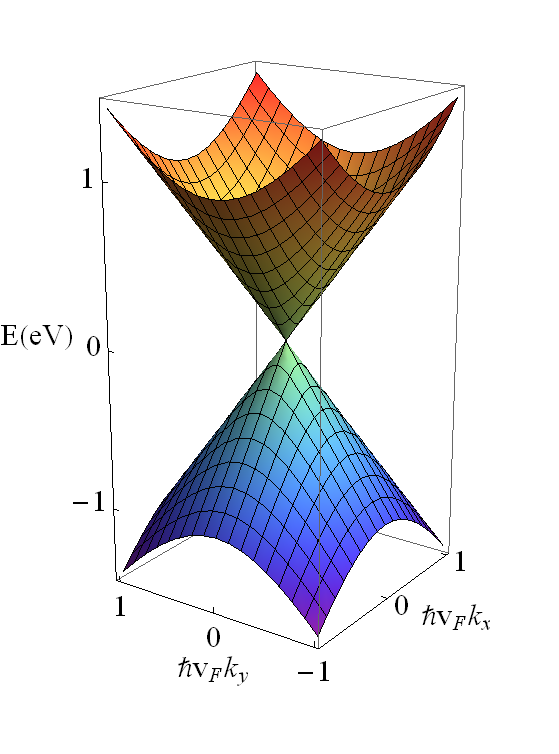
\includegraphics[width=.6\textwidth]{include/cone.png}
\caption{Dirac cone dispersion. Energy as a function of momentum, $k_x$ and $k_y$.
}\label{cone}
\end{figure}
 
 If we look closely at the spin-momentum relationship we see that it is not possible to have arbitrary spin and momentum for an electron on the TI surface. Every direction of momentum is locked to one direction of spin and vice versa. 
 %This can be seen as a broken symmetry of the surface electrons where they no longer have arbitrary spin and momentum. 
 This surface is very different from a normal metal where spin is arbitrary for any momentum and also different from a ferromagnet where the spin of an electron is fixed but can have arbitrary momentum. This coupling along with the relativistic energy dispersion is unique and provides a playground for many exotic properties. These include Majorana fermions\cite{fu_superconducting_2008,hasan_colloquium:_2010,linder_unconventional_2010,qi_topological_2011}, barrier transmission \cite{seo_transmission_2010}, spin-currents \cite{yazyev_spin_2010,burkov_spin_2010}, Aharanov-Bohm oscillations \cite{peng_aharonov-bohm_2010}, Shubnikov-de Haas oscillations \cite{analytis_bulk_2010}, Landau level quantization \cite{cheng_landau_2010}, massive relativistic Dirac fermions \cite{liu_magnetic_2009, lu_massive_2010}, and exciton condensation \cite{seradjeh_exciton_2009}.
 
In 2008, Hassan's group found a 3D TI in the form of Bi$_{.9}$Sb$_{.1}$ by way of ARPES measurements\cite{hsieh_topological_2008}. They found a linear dispersion, Dirac crossing, on the surface and while the bulk has a gapped energy spectrum. This experiment was motivated by several theoretical predictions\cite{fu_topological_2007,fu_topological_2007-1} to find topological insulators in such a 3D binary compound due to the spin-orbit coupling in the material. This led to the discovery of other TIs; Bi$_2$Se$_3$, Bi$_2$Te$_3$, Sb$_2$Te$_3$; as well as finding topological properties of pure Sb\cite{hsieh_tunable_2009,hsieh_observation_2009,hsieh_observation_2009-1,roushan_topological_2009,seo_transmission_2010}. Since the discovery in 2008, there has been an explosion in research on topological insulators in ArXiv.org, where in years 2009, 2010, 2011, 2012 there were 100, 235, 362, 421 papers on topological insulators, respectively. 
 
This concludes our basic description of the TI. We showed how a 2D TI was produced using two copies of a QH system with opposite simultaneous magnetic fields. We then extended the idea of a 2D TI to 3D ``weak" and ``strong" TIs. We then examined the surface states to understand the relationship between the spin and momentum as well as potential implications and applications.  
 
 % A simple exercise to see the insulator-surface state behavior described, we present a simplified version of the accepted model Hamiltonian for bulk Bi$_2$Se$_3$:
 % \begin{equation}
% H= (M_0+M k^2)\tau_z + A(\sigma_x k_y - \sigma_y k_x)\tau_x +B \sigma_z k_z \tau_y,
% \end{equation}
 % where $\sigma (\tau)$ represent spin (orbital) basis, $A,B,M,M0$ represent physical parameters of the system. This Hamiltonian can be diagonalized to find energy eigenvalues of 
  % \begin{equation}
% E= \pm\sqrt{(M_0+M k^2)^2 + A^2(k_x^2 + k_y^2) +B^2 k_z^2}.
% \end{equation}
 % A three step inspection can show how two critical ingredients are needed for this to be a topological insulator. By setting $A=B=0$ and having $M_0>0$, we see that we have a trivial insulator with a band-gap of $2 M_0$. By adjusting this gap parameter to negative values, $M_0<0$, we see the valence and conduction bands intersect at $E=0$. To transition this to an insulator we can set $A \neq 0$ and $B \neq 0$, in effect turning on spin orbit coupling. We now see a gap arise and through additional steps we find that this setup is host to surface states. To find these surface states we set the form of the wave functions to be 
   % \begin{equation}
% \psi \propto e^{\Lambda z}
% \end{equation}
% as an ansatz from an assumption that $H(x,y,z=0,L)=0$ and that the surface states reside on the boundaries decay into the bulk. We also make the substitution of $k_z \rightarrow -i \partial_z$. The Hamiltonian is now in the form
  % \begin{equation}
% H= (M_0+M (k_x^2+k_x^2-\Lambda^2))\tau_z + A(\sigma_x k_y - \sigma_y k_x)\tau_x +B \sigma_z (-i)\Lambda \tau_y.
% \end{equation}
% To verify the existence of a Dirac crossing at zero energy, we diagonalize the Hamiltonian and set $k_x=k_y=E=0$ and find that there exists values for $\Lambda$:
  % \begin{equation}
% \Lambda=\pm \frac{B\pm \sqrt{B^2+4M M_0}}{2M}
% \end{equation}
% illustrating that surface states do indeed exist. 


\section{Superconductivity}

\subsection{Measurement}
Superconductivity was discovered by Heike Kamerlingh Onnes in 1911.
%is usually the first item that's discussed when the topic of superconductivity is brought up. In the discovery, Onnes 
He found that the resistance of mercury drops to zero as the temperature is lowered below 4.2K, a signature of perfect conduction. An immediate question arises, if using a typical voltmeter, as used in physics labs, and Ohm's law, $V=IR$, how can resistance or voltage be measured if they should both be zero? The answer is by using a four point probe. As seen in the diagram in Fig. \ref{measures}, the probe has four point of contact on the material. Two of the connections (1,4) have a constant, controllable current flowing through them. The other two connections (2,3), then probe the sample and measure the voltage drop. The voltage measurement device has a high impedance to minimize any flow from the sample into it. The resulting voltage drop, V, and driving current, I, then give the resistance, $R=V/I$, which along with temperature results in a temperature dependent resistance. An example measurement of Cu$_{.2}$Bi$_2$Se$_3$, a new superconducting material based on the topological insulator Bi$_2$Se$_3$, is shown in Fig. \ref{measures}. The plot shows a clear resistance drop at 3.5 Kelvin, the signature of superconductivity. 
\begin{figure}
\center
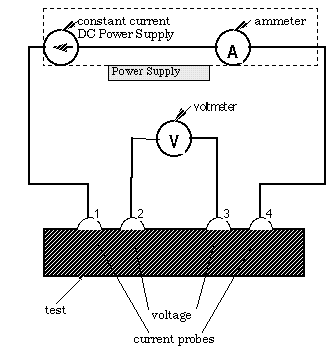
\includegraphics[width=.45 \textwidth]{include/fourprobe.png}
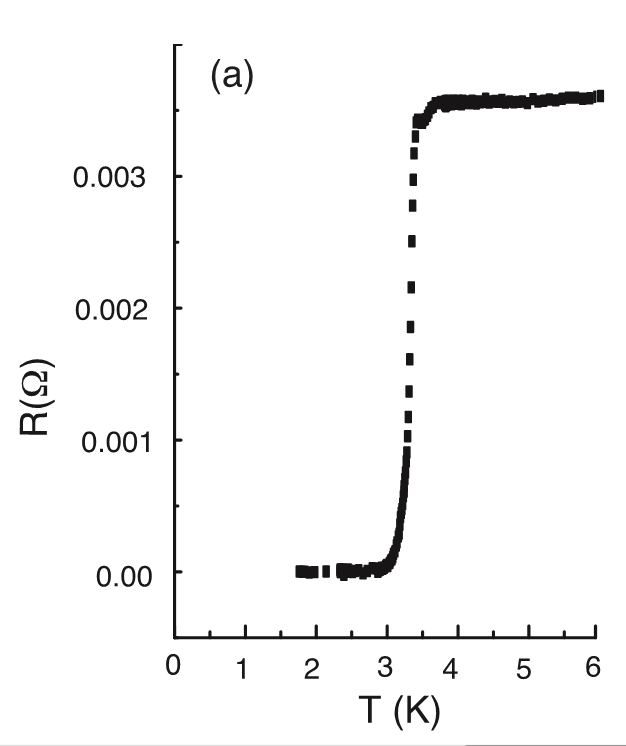
\includegraphics[width=.45 \textwidth]{include/resistance.png}
\caption{(left) Four probe measurement device. Probes 1 and 4 are used to flow a current across a sample while probes 2 and 3 measure the voltage drop across the sample where the current is flowing. (right) Resistance ($\Omega$) vs Temperature (Kelvin) experiment on Cu$_{.2}$Bi$_2$Se$_3$ from arXiv:1111.5805. The drop in resistance is a signature of superconductivity. \label{measures}
}
\end{figure}
\clearpage
\subsection{BCS and Bogoliubov Theory}
Bardeen, Cooper, and Schreiffer (BCS) came up with a theory to explain the mechanism behind superconductivity. We start with the Hamiltonian that represents a free electron system with two-body electron interactions,
\begin{equation}
H=\sum_{\bf{k},\sigma} (\epsilon_{\bf{k}}-\mu)
c^{\dagger}_{\bf{k}\sigma}
c_{\bf{k}\sigma}+
\sum_{\bf{k},\bf{l'}}
V_{\bf{k},\bf{k'}}\, 
c^{\dagger}_{\bf{k}\uparrow}
c^{\dagger}_{-\bf{k}\downarrow} 
c^{}_{-\bf{k'}\uparrow}
c^{}_{\bf{k'}\downarrow}
\end{equation}
where $c^{\dagger}_{\bf{k}\sigma}$ ($c_{\bf{k}\sigma}$) is the electron creation (annihilation) operator, the summations are over spin ($\sigma$)and momentum ($\bf{k},\bf{k'}$), $\epsilon_{\bf{k}}$ is the free electron energy, $V_{\bf{k,k'}}$ is the electron-electron interaction potential. The commutation relations for the fermion creation and annihilation operators are
\begin{equation}
\{c^{\dagger}_{\bf{k}\sigma},c_{\bf{k'}\sigma'}\}_+=\delta_{\bf{k},\bf{k'}}\delta_{\sigma \sigma'}
\end{equation}
\begin{equation}
\{c^{\dagger}_{\bf{k}\sigma},c^{\dagger}_{\bf{k'}\sigma'}\}_+=\{c_{\bf{k}\sigma},c_{\bf{k'}\sigma'}\}_+=0.
\end{equation}

In usual electron systems, the Coulomb interaction between electrons is repulsive, but the effective interaction can become attractive. 
% scattering potential, $V_{\bf{k k'}}$, usually positive, represents repulsive interactions. But as the temperature is lowered, what BCS explained was that the repulsive interaction was no longer the dominant interaction. Instead, what occurs at zero temperature is the following. 
As an electron passes through a lattice of low-mobility nuclei, they actually cause the nuclei to shift causing a phonon interaction with electron. This phonon interaction can be strong enough to effectively attract, $V_{\bf{k k'}}<0$, two electrons with opposite momenta($\bf{k},-\bf{k}$). From the Pauli exclusion principle, we seek a bound pair of electrons with zero total momentum and antisymmetric wave functions known as a Cooper pair. When the electrons pair, they form a condensate of the bosons, which supports superflow that is responsible for the lack of resistance. 
The electrons near the Fermi energy are most susceptible to pairing, usually when they are within some Debye energy cutoff, $\hbar \omega_D$. One way to describe the superconductor is through a condensate wave function or more precisely the superconducting order parameter, $\Delta(\bf{x})$, or $\Delta_{\bf{k}}$. This function is found by a mean field approach to the pairing potential, $V_{\bf{k k'}}$, through the gap equation
\begin{equation}
\Delta_{\bf{k}}=\sum_{\bf{k'}}
V_{\bf{k k'}}\,
c^{}_{-\bf{k'}\uparrow}
c^{}_{\bf{k'}\downarrow}
\end{equation}
reducing the Hamiltonian down to 
\begin{equation}
H=\sum_{\bf{k},\sigma} (\epsilon_{\bf{k}}-\mu)
c^{\dagger}_{\bf{k}\sigma}
c_{\bf{k}\sigma}+
\sum_{\bf{k}}
\Delta_{\bf{k}}\, 
c^{\dagger}_{\bf{k}\uparrow}
c^{\dagger}_{-\bf{k}\downarrow} +
h.c.
\end{equation}
To diagonalize this Hamiltonian we change the basis, where rather than restricting ourselves to operators of electrons, we use the Bogoliubov-de Gennes (BdG) transformation to introduce the operators on quasiparticle excitations of particles and holes. This is done through
\begin{equation}
c_{\bf{k}\sigma} = \sum_n u_{n \bf{k} \sigma} \gamma_{n\bf{k}}+v^\ast_{n \bf{k} \sigma} \gamma^\dagger_{n\bf{k}},\quad
c_{\bf{k}\sigma}^\dagger = \sum_n u_{n \bf{k} \sigma}^\ast \gamma_{n\bf{k}}^\dagger+v_{n \bf{k} \sigma} \gamma_{n\bf{k}}
\end{equation}
where the quasiparticle operators fulfill the anti-commutation relations,
\begin{equation}
\{\gamma^\dagger_{\bf{k}\sigma},\gamma_{\bf{k'}\sigma'}\}=\delta_{\bf{kk'}}\delta_{\sigma\sigma'} ,\qquad 
\{\gamma_{\bf{k}\sigma},\gamma_{\bf{k'}\sigma'}\}=
\{\gamma^\dagger_{\bf{k}\sigma},\gamma^\dagger_{\bf{k'}\sigma'}\}=0
\end{equation}
and allow us to diagonalize the Hamiltonian as
\begin{equation}
H=E_0+\sum_{\bf{k},\sigma} E_{\bf{k}}
\gamma^{\dagger}_{\bf{k}\sigma}
\gamma_{\bf{k}\sigma}.
\end{equation}
The quasiparticle (quasihole) wave function is $u_{\bf{k}\sigma}$ ($v_{\bf{k}\sigma}$). Each electron creation/annihilation operator is a superposition of a quasiparticle creation and annihilation operator. The inverse of this transformation,
\begin{equation}
\gamma_{\bf{k}\sigma} = \sum_n u_{n \bf{k} \sigma} c_{n\bf{k}}-v^\ast_{n \bf{k} \sigma} c^\dagger_{n\bf{k}},\quad
\gamma_{\bf{k}\sigma}^\dagger = \sum_n u_{n \bf{k} \sigma}^\ast c_{n\bf{k}}^\dagger-v_{n \bf{k} \sigma} c_{n\bf{k}}
\end{equation}
 leads to each quasiparticle operator being a superposition of the electron creation operator and the hole creation operator. This physical interpretation allow us to see that there is more to the story than just electrons and holes, but electron-like and hole-like quasiparticle excitations.

The form of the BdG Hamiltonian is 
\begin{equation}
H_{B}=\left( \begin{array}{cc}
\epsilon_{\bf{k}}-\mu   &-\hat{\Delta}_{\bf{k}}\, i\sigma_y\\ 
\hat{\Delta}^{\dagger}_{\bf{k}} \, i\sigma_y &  \mu-\epsilon_{\bf{k}}
 \end{array} \right), \label{bdgHH} 
\end{equation}
in the basis of 
\begin{equation}
\psi=\left(
u_{\bf{k}\uparrow},
u_{\bf{k}\downarrow},
v_{\bf{k}\uparrow},
v_{\bf{k}\downarrow}\right)^T.
\end{equation}
The $\hat{\Delta}_{\bf{k}}$ can come in a variety of forms, strictly depending on the pairing symmetry of the superconductor. Generally it can be written as $\Delta_{\bf{k}}=\Delta_0(\bf{k})+\bf{d}(\bf{k})\cdot \bf{\sigma}$, while in the BCS case, we focus on $\Delta_{\bf{k}}=\Delta_0$, a constant value, representing s-wave orbital pairing\cite{mineev_introduction_1999}. This allows us to find the eigen values of the system,
\begin{equation}
E_{\bf{k}}=\pm\sqrt{(\epsilon_{\bf{k}}-\mu)^2 + |\Delta|^2}.
\end{equation}
where the spectrum can be seen in the Fig. \ref{bcsplot}. There is now a finite gap of size $2\Delta_0$ seen centered about 0. The gap is a result of the pairing that occurs in the superconductor. These paired states form the condensate and no low energy excitations can exist within the energy gap in the spectrum. In order to have an excitation out of the condensate, you would need $2\Delta_0$ energy to break the pair. 


\begin{figure}
\center
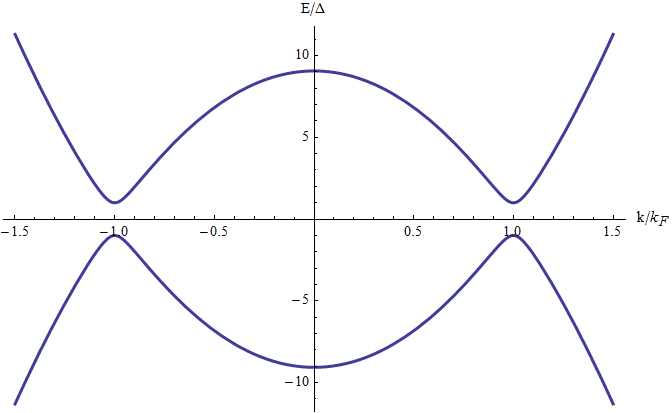
\includegraphics[width=.95 \textwidth]{include/bcsplot.png}
\caption{Energy spectrum for a BCS superconductor with a gap of $2\Delta_0$ and $\mu/\Delta_0=10$.
} \label{bcsplot}
\end{figure}

This concludes the introduction to superconductivity. Here, we reviewed  the BCS theory on superconductivity to describe the mechanism behind the Cooper pairing, and diagonalizing the BCS Hamiltonian using a mean field approximation and the Bogoliubov-de Gennes Transformation to obtain the energy spectrum. These are the building blocks for understanding the discussions on superconductivity in this thesis. 

\section{Topological Superconductors and Superconductor-Topological Insulator Heterostructures}
This section presents two related condensed matter systems that have exotic properties and the motivation for studying them. These are p$_x$+ip$_y$ superconductors and topological insulator-superconductor heterostructures that host Majorana Fermions. These systems have implications in understanding the role of topology in superconducting systems as well as the possibility of topological quantum computation through the Majorana Fermion. This thesis can be viewed as a systematic deeper study of the latter systems beyond phenomenology. 
\subsection{p$_x$+ip$_y$ superconductors}
One kind of a superconductor that has exotic topological behavior is the p$_x$+ip$_y$ superconductor. The symmetry of this paired spin-triplet state is of the form $\hat{\Delta}_k=\Delta_0 (k_x+ik_y) (\sigma_x+i\sigma_y)$. If we apply this form of the pairing into \eqref{bdgHH}, we can diagonalize the BdG Hamiltonian and find eigenvalues of the form

\begin{equation}
E_{\bf{k}}=\pm\sqrt{(\epsilon_{\bf{k}}-\mu)^2 + (\Delta_0|\bf{k}|)^2}.
\end{equation}
This differs from the conventional s-wave eigen energies because the gap term now depends on $\bf{k}$. For values of $\mu>>0$, this doesn't effect the spectrum by any more then a negligible change. The noticeable difference, as described Read and Green\cite{RG}, is when the Fermi energy is reduced to a small value so that $(\epsilon_{\bf{k}}-\mu) \rightarrow -\mu$. The spectrum then evolves into a spectrum for a relativistic Dirac fermion with mass $\mu$ and speed of light $\Delta_0$. We also write the BdG equations in the form of
\begin{eqnarray}
E u=-\mu u + \Delta^\ast i (\partial_x + i \partial_y) v\\
E v=\mu v + \Delta i (\partial_x - i \partial_y) u.
\end{eqnarray}
This is a form of the Dirac equation, and the BdG equations allow for $u=v^\ast$ through charge conjugation symmetry, where at each $\bf{k}$ there is only one excitation mode. This shows that the particles, $u$, are their own anti-particles, $v$. When a Dirac fermion has this property, it is a Majorana Fermion. Now consider a setup for this system where the mass term varies spatially through a a domain wall ($ \mu(x)\propto \text{sign}(x-x_0)$), by tuning the Fermi energy spatially. The requirement for the domain wall is due to the parameter (x) dependent transition from a trivial state superconductor, $\mu<0$ to a non trivial topological superconductor, $\mu>0$. One simple model to do this is by $\mu(x)=\mu \sin(2 \pi x/L)$. We find a spectrum with linear modes in Fig. \ref{pmajorana}. The linear Majorana modes are found to have chiral propagation and reside at the centers of the domain walls. Another way to host a Majorana in a p-wave superconductor is by imposing a vortex through a magnetic field, where at the core of the vortex reside the Majorana modes. 


\begin{figure}[h]
\center
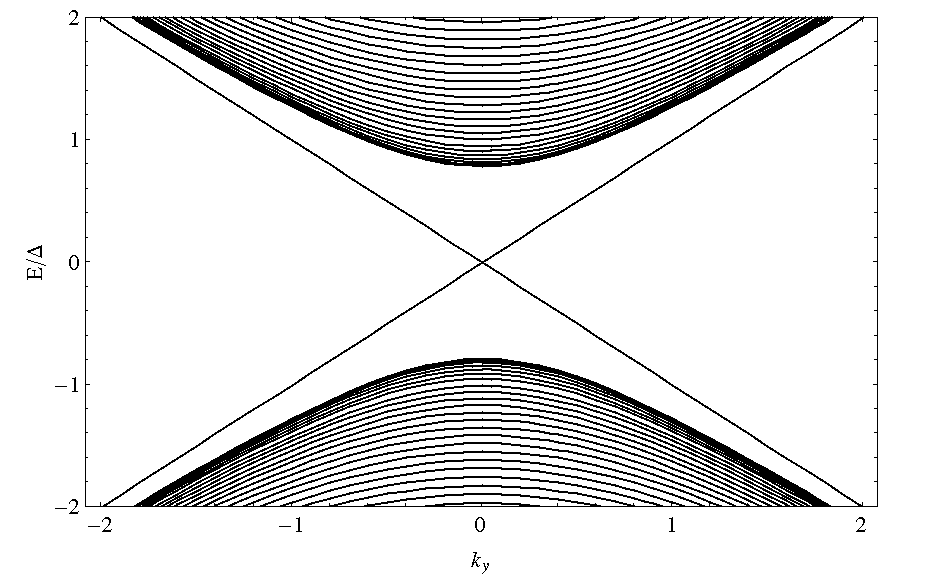
\includegraphics[width=.95 \textwidth]{include/pmajorana.png}
\caption{Energy spectrum for a $p_x\pm ip_y$ superconductor with a chemical potential domain wall, ensuring linearly dispersing Majorana modes.
} \label{pmajorana}
\end{figure}

\subsection{Fu-Kane Superconductor/Topological Insulator Model}
Fu and Kane were the first to describe the effect of a superconductor in close proximity to the surface of a TI\cite{majorana}. The TI has the Hamiltonian in the form of $H=v_F(\sigma_x k_y-\sigma_y k_x) - \mu$, where $k_i$ are the momenta, $\sigma_i$ are the Pauli spin matrices, and $v_F$ is the Fermi velocity. If an $s-$wave superconductor is brought to the surface of the TI, Fu-Kane argued that pairing interaction between electrons will be induced on the surface. 

This interplay between a TI and S presents many possibilities of various physical effects. This system can be seen to mimic a spin-less $p_x\pm ip_y$ superconductor. Also, under certain conditions where there is a domain wall through the superconductor order parameter, $\Delta$ or a magnetic domain wall, it is expected to find a Majorana mode. 

Fu-Kane argued that the form of the pairing term is consistent from the S side to the TI side producing the following BdG Hamiltonian
\begin{equation}
\mathcal{H}(\mathbf{k})=\left(
\begin{array}{cc}
H(\mathbf{k})  &  i\sigma_y  \Delta \\
-i\sigma_y \Delta^*  &   - H^*(-\mathbf{k})
\end{array}
\right)=v_F(\sigma_x k_y-\tau_z\sigma_y k_x) - \tau_z\mu +\tau_y\sigma_y\Delta.
\end{equation}

The spectrum for this system is
\begin{equation}
E=\sqrt{|\Delta|^2 +(v_F |\bf{k}|\pm \mu)^2}.
\end{equation}
This system is very analogous to the p-wave superconductor. If we take the limit $\mu\rightarrow 0$ this dispersion is also relativistic where the mass term is $\Delta$ and the speed of light is $v_F$. The $p_x\pm ip_y$ term is responsible for the resulting Majorana mode. In the superconductor-TI heterostructure, this term is also, as we shall see soon, responsible for producing Majorana modes.
Since the mass term is parameter, it can be tuned to close the gap at one (or an odd number of points) in the spectrum. The mass term in the S-TI system is the gap parameter, $\Delta$. If we allow $\Delta$ to flip sign spatially from a positive value, $|\Delta_0|$, to a negative value, $-|\Delta_0|$, for example through $\Delta(x)=\Delta_0 \tanh( x/L)$, we find a Majorana mode localized at the point where $\Delta(x)=0\, (x=0)$ with a linear dispersion that resembles the spectrum of the p-wave superconductor edge-state in Fig. \ref{pmajorana}. One difference is the TI version is four-fold degenerate (particle/hole) of the $E=0$ mode while the p-wave is two-fold degenerate (particle/hole). Both systems' linear dispersing states are localized at the domain wall, $x=0$. This domain wall can be seen as a Majorana wire in the y-direction.

We've now shown some superconductors with exotic properties. We looked at the p-wave superconductor and how it can be tuned to host Majorana modes along with its relativistic Dirac-like energy dispersion. We also looked at the TI-S heterostructure proposed by Fu and Kane which can be tuned to host Majorana modes. These systems are very analogous to each other and show the potential of engineering topological superconductivity using the hybrid structures of TI and $s-$wave superconductors. The Fu-Kane will be the starting point for latter two thirds of the thesis where we study TI-S structures in greater detail.



\chapter{Metal to Topological Insulator Scattering}

As described in Chapter 1, the topological insulator (TI) has a unique surface where the spin and momentum of an electron are coupled such that the direction of the spin is equal to the direction of the momentum plus $\pi/2$. That is to say, the electron's wave function, $\ket{\psi_{\bf{k}}}$, is presented as
\begin{equation}
\ket{\psi_{\bf{k}}}=\pm i e^{-i \theta}\ket{\uparrow}+\ket{\downarrow}
\end{equation}
where $\theta=\arctan\left(k_y/k_x\right)$ and $\ket{\uparrow} (\ket{\downarrow})$ is the spin up (down) state. It's clear that the phase $i e^{-i \theta}$ dictates the direction of the spin in the $x-y$ plane. 
This special surface is the motivation for the following chapter. 

Since we understand the spin-momentum behavior of the electrons that reside on the surface of the TI, a natural extension would be to understanding electrons that scatter off the surface of a TI. Any incoming electron has an interaction with the spin-orbit coupling of the TI. This interaction dictates the resulting spin of the reflected electron. 

We find that for a certain critical angle, the electron's spin will always flip, regardless of its state before reflection (i.e. $\alpha\ket{\uparrow}+\beta\ket{\downarrow}\rightarrow\alpha\ket{\downarrow}+\beta\ket{\uparrow}$). This is very different from reflection from a ferromagnetic insulator, where the spin directions of incoming polarized electrons are rotated by the exchange field \cite{toku}. This clear difference is unique and allows for an ability to control electrons arbitrarily and perform NOT-gate like operations in binary logic devices, (i.e. TRUE$\rightarrow$FALSE and FALSE$\rightarrow$TRUE). 

To understand this spin dependent interaction we theoretically study a metal-TI interface. The left half, spatially, is a metal and the right half is the TI. An incoming electron comes from the metal side and travels to the TI surface. Since the TI is an insulator, incoming electrons do not propagate through but rather reflect back to the metal side. We calculate the spin dependent reflection coefficients of the reflected electron. This spin-resolved reflection has implications in using TIs for spintronics because of the ability to invert the spin direction, hence negate the information stored on there.

In addition to the scattering approach, we seek to understand what the combined effect is when a metal and TI are in contact with each other in a different perspective. We do this by using a lattice Green's function method to find the resulting spatially resolved energy spectrum and to calculate the scattering coefficients, also. We find that the local spectrum has two limits depending on the strength of the tunneling between the metal and TI. For good tunneling we find that the metal has a stronger influence on the spectrum near the surface whereas for weak contacts the Dirac cone is clear and well-defined. 

Lastly, we discuss the complex energy spectrum of the TI ($E(k_{\text{Real}} , k_{\text{Imag}})$, $k_z \rightarrow k_{\text{Real}} + i k_{\text{Imag}}$). It gives us insight into understanding the behavior of the surface localized wave function of the Dirac electrons. 

\section{Introduction}
Recently discovered three dimensional topological band insulators \cite{fu07,moore,roy}, such as Bi$_{1-x}$Sb$_x$ \cite{Hsieh2008} and Bi$_2$Se$_3$ \cite{Xia09,zhang2009,Chen09}, are spin-orbit coupled crystal solids with a bulk gap but protected gapless surface states. The low energy excitations at the surface are helical Dirac fermions, i.e., their spin and momentum are entangled (locked) \cite{Hsieh2009}. The charge and spin transport on the surface of a topological insulator
are intrinsically coupled \cite{burkov}.
This makes these materials a promising new platform for spintronics. In addition, heterostructures involving topological insulator, superconductor, and/or ferromagnet have been predicted to show a remarkable array of spectral and transport properties (for review
see Ref. \cite{today,rmp,Qi-zhang-rev}). 

Electronic or spintronic devices based on topological insulators will almost inevitably involve metal as measurement probes or functioning components \cite{yokoyama09}. This motivates us to study the local spectrum near the interface between a metal (M) and a topological insulator (TI). For a metal-ordinary semiconductor junction with good contact, it is well known that the metallic Bloch states penetrate into the semiconductor as evanescent waves localized at the interface (for energies within the band gap). Such interface states are known as metal induced gap states (MIGS) \cite{heine65,cohen}. They play an important role in controlling the junction properties, e.g., by pinning the semiconductor Fermi level to determine the Schottky barrier height \cite{tersoff}, a key parameter of the junction.

The local spectrum at the M-TI junction is intimately related to the spin-active scattering of electrons at the M-TI interface. In this chapter, we systematically study the evolution of the scattering matrix and the interface spectra
with the junction transparency and metal Fermi surface parameters. 
%by exploiting the {\it complex band structure} of topological insulators, which describes the decaying (rather than propagating Bloch wave) solutions of the crystal Hamiltonian.
The scattering matrix \cite{mrs} we obtain here also forms the basis to investigate the details of the superconducting proximity effect near the superconductor-TI interface \cite{stan}, which was shown by Fu and Kane to host Majorana fermions \cite{majorana}.

The scattering at the M-TI interface differs significantly from its two dimensional analog, the interface between a metal and a quantum spin Hall (QSH) insulator studied by Tokoyama et al \cite{yokoyama09}. They predicted a giant spin rotation angle $\alpha\sim \pi$ and interpreted the enhancement as resonance with the one-dimensional helical edge modes. By contrast, for M-TI interface we predict a critical incident angle at which complete spin flipping occurs and the spin rotation angle jumps by $\pi$. We will explain its origin, {in particular its relation to the surface helical Dirac spectrum}, and discuss its spintronic implications.

This chapter is organized as follows. 
We will first compute the scattering matrix using a $\mathbf{k\cdot p}$ continuum model 
by matching the envelope wave functions at the M-TI interface. This simple calculation is easy to understand, 
and it brings out
the main physics of our problem. Along the way, we will discuss the complex band structure of Bi$_2$Se$_3$,
 which describes the decaying (rather than propagating Bloch wave) solutions of the crystal Hamiltonian.
The various caveats of this calculation 
are then remedied by considering a much more general lattice model. Most importantly, it enables us to 
track how the scattering matrix and interface spectrum change with interface transparency. It also sheds light on
the origin of perfect spin-flip scattering at the critical angle.
We will show that the results obtained from these two complementary methods are consistent with each.

\section{Model Hamiltonian and Complex Band Structure}

We consider Bi$_2$Se$_3$ as a prime example of 3D strong topological insulators. Its low energy $\mathbf{k\cdot p}$ Hamiltonian was obtained by Zhang et al \cite{zhang2009},
\[
\hat{H}_{TI}(\v{k})=\epsilon_0(\v{k})\hat{1}+\sum_{\mu=0}^{3}d_\mu(\v{k})\hat{\Gamma}_\mu.
\]
Here $d_0(\v{k})=M-B_1k^2_z-B_2(k_x^2+k_y^2)$, $d_1(\v{k})=A_2 k_x$, $d_2(\v{k})=A_2 k_y$, $d_3(\v{k})=A_1 k_z$, and $\epsilon_0(\v{k})=C+D_1k_z^2+D_2(k_x^2+k_y^2)$. The numerical values of $M$, $A$, $B$, $C$, $D$ are given in Ref. 
\cite{zhang2009}.
We choose the basis ($\ket{+\uparrow}$, $\ket{+\downarrow}$, $\ket{-\uparrow}$,$\ket{-\downarrow}$), where $\pm$ labels the hybridized $p_z$ orbital with even (odd) parity \cite{zhang2009}. The Gamma matrices are defined as
$\hat{\Gamma}_0=\hat{\tau}_3\otimes \hat{1}$, $\hat{\Gamma}_i=\hat{\tau}_1\otimes \hat{\sigma}_i$, with
$\hat{\tau}_i$ ($\hat{\sigma}_i$) being the Pauli matrices in the orbital (spin) space.
The chemical potential of as-grown Bi$_2$Se$_3$ crystal actually lies in the conduction 
band \cite{Hsieh2009}. By hole doping \cite{Hsieh2009} 
or applying a gate voltage \cite{gate}, the chemical potential can be tuned inside 
the gap. The system is well described by $H_{TI}$ (note that energy zero is set as 
in the middle of the band gap).

In this section, we first adopt a rather artificial model for metals with negligible 
spin-orbit coupling. It is
obtained by turning off the spin-orbit interaction (setting $d_\mu=0$ for $\mu$=1,2,3) 
in $H_{TI}$ and shifting the Fermi level into 
the conduction band. The result is spin-degenerate two-band Hamiltonian
\[
\hat{H}_M(\v{k})=[\epsilon_0(\v{k})-E_F]\hat{1}+d_0(\v{k})\hat{\Gamma}_0.
\]
Its band structure, schematically shown in Fig. 1(b), consists of two oppositely dispersing bands 
(the solid and dash line). $E_F$ is tuned to be much higher than the band crossing point, so
the scattering properties of low energy electrons near the Fermi surface are 
insensitive to the band crossing at high energies. This claim will be verified later using a
more generic model for the metal. A similar model was used in the study of metal-QSH interface \cite{yokoyama09}.

%%%%%%%%%%%%%%%%%%%%%%%%%%

\begin{figure}
\center
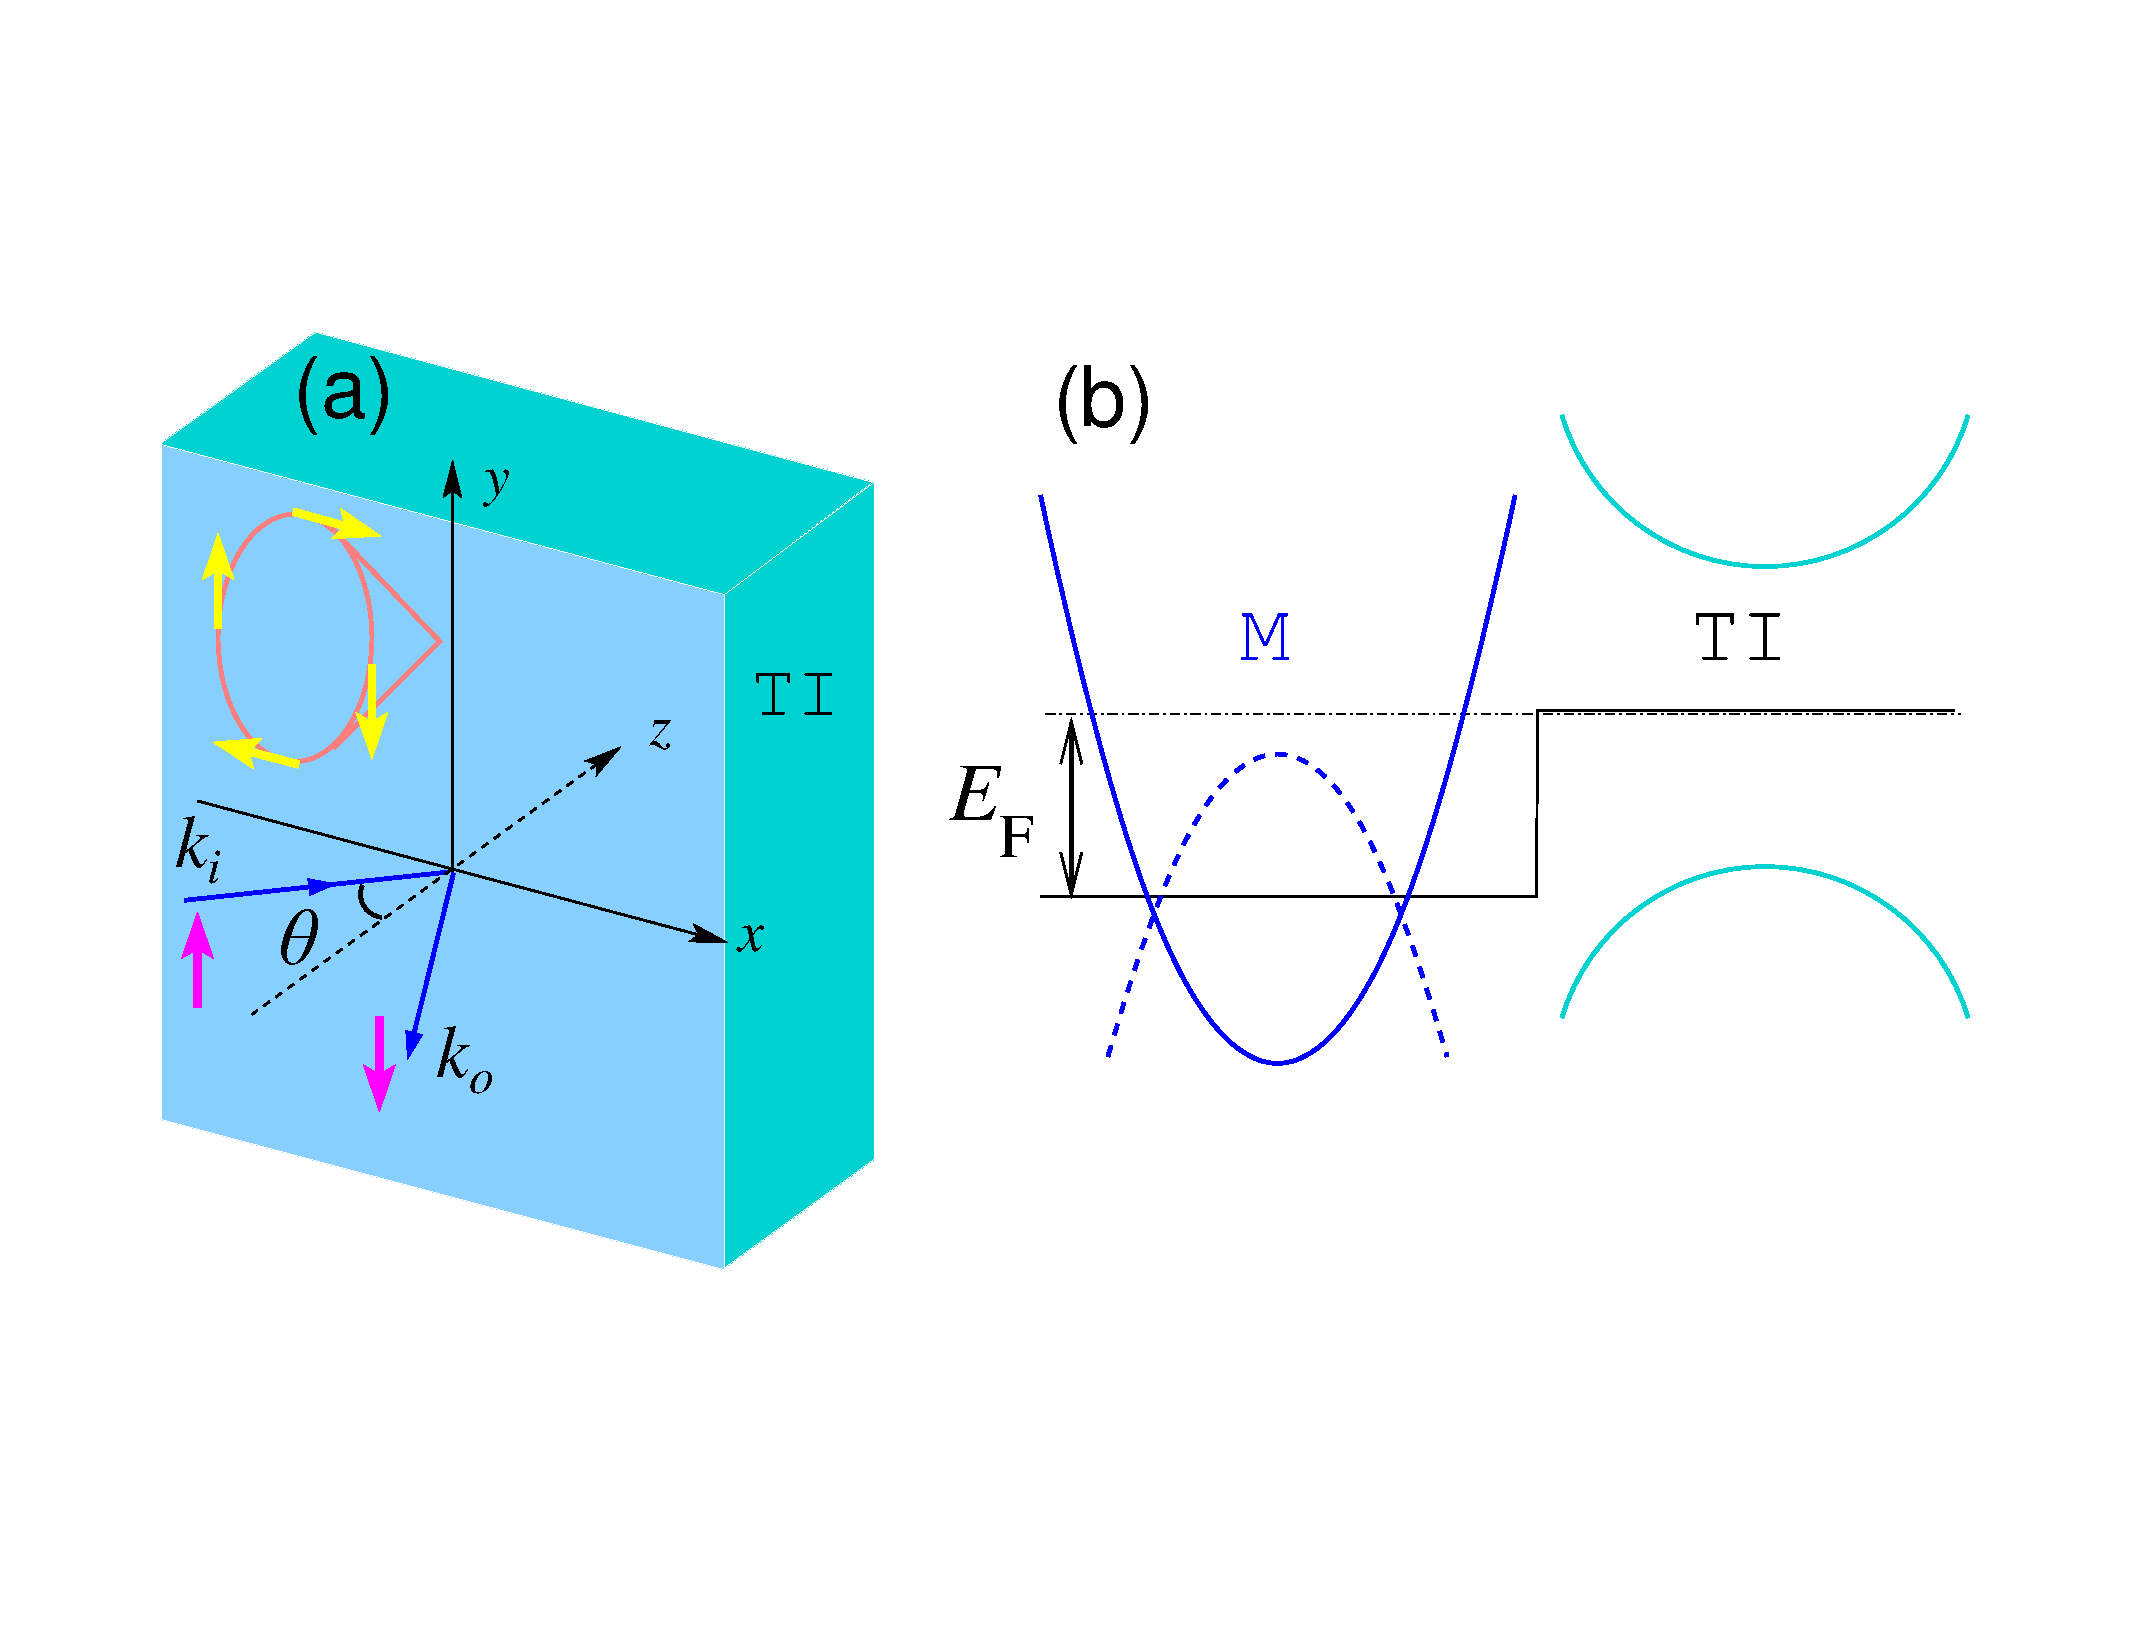
\includegraphics[width=\textwidth]{include/geometry.pdf}
\caption{(a) Scattering geometry at a metal (M)-topological insulator (TI) interface.
(b) Schematic band structure of the metal (modeled by $\hat{H}_M$) and topological insulator.
}
\end{figure}
%%%%%%%%%%%%%%%%%%%%%%%%%%


Matching the wave functions of two dissimilar 
materials (such as Au and Bi$_2$Se$_3$) at interface is in general 
complicated within the $\mathbf{k\cdot p}$ formalism, because the envelope wave functions 
on either side are defined using different basis (see Ref. \cite{bc} and reference therein). 
For the particular model $H_M$, however, such complication
is circumvented. Then, then wave functions at the metal-TI interface ($z=0$) satisfy the Ben-Daniel 
and Duke boundary condition \cite{duke}, 
\[
\hat{\Phi}_M=\hat{\Phi}_{TI}, \;\;\; \hat{v}_M \hat{\Phi}_M = \hat{v}_{TI}\hat{\Phi}_{TI}.
\]
Here $\hat{\Phi}_i$ is the four-component wave function, and 
the velocity matrix $\hat{v}_{i}=\partial \hat{H}_i/\partial k_z$, $i\in \{M, TI\}$. 
Such boundary condition assumes good atomic contact between two materials.

We are interested in energies below the band gap of TI, so 
$\hat{\Phi}_{TI}$ is evanescent in nature and only penetrates into TI 
for a finite length. Such localized (surface or interface) 
states inside topological insulator can be treated within the $\mathbf{k\cdot p}$ formalism 
using the theory of {\it complex band structures}, pioneered by Kohn \cite{kohn59}, Blount \cite{blount62}, 
and Heine \cite{heine63} et al. 
The main idea is to allow the crystal momentum to be complex and analytically continue
$H_{TI}(\v{k})$ to the complex $\v{k}$ plane. 
While the extended Bloch waves are the eigen states of $H_{TI}(\v{k})$ for real $\v{k}$, 
eigen functions of $H_{TI}(\v{k})$ for complex $\v{k}$ describe localized states. Together they
form a complete basis to describe crystals of finite dimension. 

%%%%%%%%%%%%%%%%%%%%%%%%%%
\begin{figure}
\center
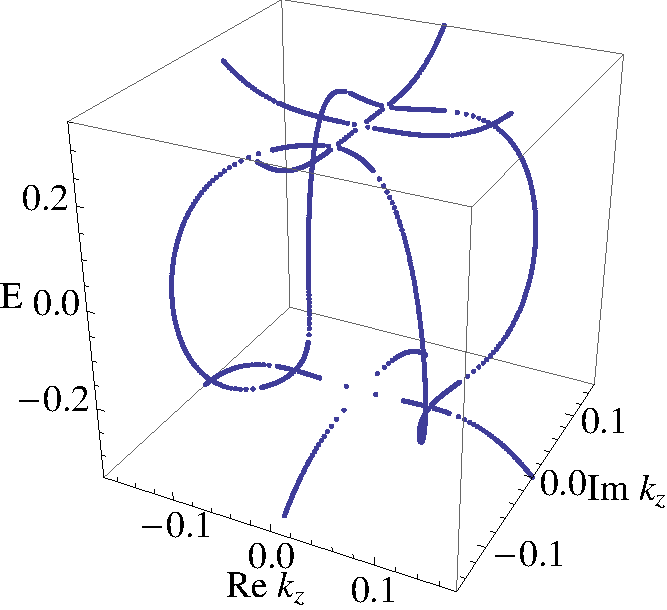
\includegraphics[width=.45 \textwidth]{include/f2.pdf}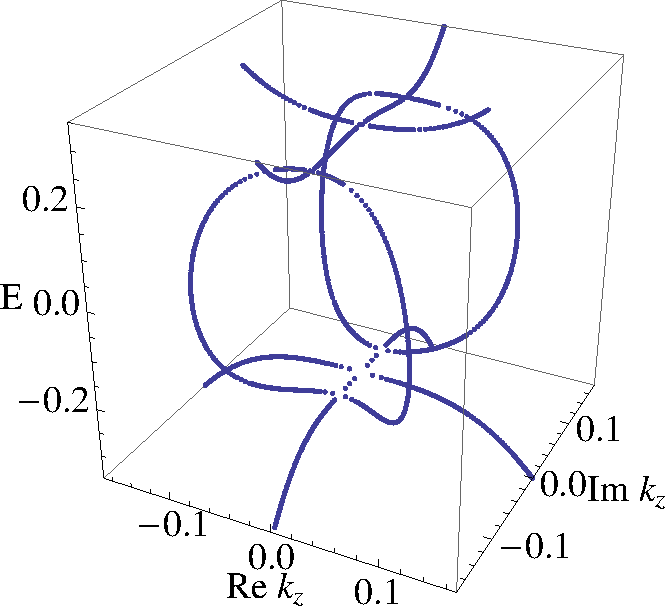
\includegraphics[width=.45 \textwidth]{include/f4.pdf}
\caption{The complex band structure
of topological insulator described by $\hat{H}_{TI}(\v{k})$ 
for $k_y=0$, $k_x=0.02$ (left) and $0.04$ (right). $E$ is measured in eV, and $k$ in \AA$^{-1}$.
Subgap states with complex $k_z$ represent evanescent waves. 
The topology of  real lines \cite{heine63}  changes as $k_x$ is increased.  
}
\end{figure}
%%%%%%%%%%%%%%%%%%%%%%%%%%

In our scattering problem, we have to find all eigen states of $H_{TI}(\v{k})$ with energy $E$ and 
wave vector $\v{k}=(k_x,k_y,\tilde{k}_z)$, where $k_x$ and $k_y$ are given and real, but $\tilde{k}_z$ is 
complex and unknown. For a general $\mathbf{k\cdot p}$ Hamiltonian such as $\hat{H}_{TI}$, 
we follow Chang and Schulman \cite{chang82} to rewrite it as
\[
\hat{H}_{TI}=\hat{h}_0(k_x,k_y)+\hat{h}_1 \tilde{k}_z+\hat{h}_2\tilde{k}^2_z,
\]
where $\hat{h}_1=A_1\hat{\Gamma}_3$, and $\hat{h}_2=-B_1\hat{\Gamma}_0$. 
Then the eigen equation $(\hat{H}_{TI}-E\hat{1})\hat{\phi}=0$ can be reorganized into an 
eigen value problem for $\tilde{k}_z$,
\[
\left(
\begin{array}{ll}
  0 & 1   \\
  -\hat{h}_2^{-1}(\hat{h}_0-E\hat{1}) & -\hat{h}_2^{-1}\hat{h}_1
  \end{array}
\right)
\left(
\begin{array}{l}
  \hat{\phi}   \\
  \hat{\phi}'  
\end{array}
\right)
=\tilde{k}_z \left(
\begin{array}{l}
  \hat{\phi}   \\
  \hat{\phi}'    
\end{array}
\right).
\]
%%% note: these details can be omitted to save space 
Then all possible values of $\tilde{k}_z$ can be obtained for given incident parameter $E$, $k_x$, and $k_y$. 
For the anisotropic Dirac Hamiltonian $H_{TI}(\v{k})$, the energy eigenvalues can be obtained 
analytically \cite{qi_field}, which allows for an analytical solution of the complex band structure.

For $E$ within the gap, there are in general 4 pairs of complex solution of $\tilde{k}_z$, for if $\tilde{k}_z$ is a solution so is $\tilde{k}^*_z$. 
We label those with positive imaginary parts with $\{\tilde{k}^\nu_z\}$, and the corresponding wave function $\{\hat{\phi}^\nu \}$, $\nu=1,2,3,4$. They are decaying solutions in the half space $z>0$. In our model, $\tilde{k}_z$ turns out to be doubly degenerate, as shown in Fig. 2. The wave function inside TI ($z>0$) then has the form
\[
\hat{\Phi}_{TI}=\sum_{\nu} t_\nu e^{i\tilde{k}^\nu_z z} \hat{\phi}_\nu.
\]

\section{Scattering Matrix from Wave-Function Matching} 

To set the stage for discussing scattering off a topological insulator, it is instructive to recall the generic features of elastic scattering of electrons by a heavy ion with spin-orbit interaction. This classical problem was solved by Mott, and known as {\it Mott scattering}. 
%It is being used, for example, to measure the spin polarization of photo electrons in spin-resolved ARPES. 
% Spin-orbital coupling amounts to a momentum dependent magnetic field $\mathbf{B}(\mathbf{k})$, which causes the spin of incident electron to precess. 
The scattering matrix has the general form \cite{mott}
\[
\hat{S}_{Mott}=u\hat{1}+w\hat{{\boldsymbol{\sigma}}}\cdot (\mathbf{k}_{i}\times \mathbf{k}_{o}),
\]
where $\mathbf{k}_{i}$ and $\mathbf{k}_{o}$ are the incident and outgoing momentum respectively, $\hat{\boldsymbol{\sigma}}$ is the Pauli matrix, and $u,w$ depend on the scattering angle. It is customary to
define the spin-flip amplitude $f=S_{21}$, and spin-conserving amplitude $g=S_{11}$. 
Both $f$ and $g$ are complex numbers, their relative phase defines the {\it spin rotation angle} $\alpha=\mathrm{Arg}(g^*f)$.
One immediately sees that for back scattering, $\hat{S}_{Mott}=u\hat{1}$, so there is no spin flip, $f=0$. As we will show below, this also holds true for scattering off TI.

Now consider an electron coming from the metal 
with momentum $\v{k}$ incident on the M-TI interface located at $z=0$, 
as schematically shown in Fig. 1(a). 
We assume the interface is 
translationally invariant, so the transverse momentum $\v{k}_{\parallel}=(k_x,k_y)$ is 
conserved, and the energy $E$ of the electron 
lies within the band gap of TI. Then, only total reflection 
is possible, but the spin-orbit coupling inside TI acting like a $\v{k}$-dependent magnetic field rotates the spin of the incident particle. The scattering (reflection) matrix has the form
\[
\hat{S}(\v{k})=\left(
\begin{array}{ll}
  g & \bar{f}   \\
  f & \bar{g}
  \end{array}
\right),
\]
where $|g|^2+|f|^2=1$. 
Our goal is to find the dependence of the scattering amplitudes $f,g$ 
on $\v{k}$, or equivalently, on energy $E$ and 
incident angle $\theta$. From time-reversal symmetry, 
$\bar{f}(E,\theta)=f(E,-\theta)$ and $\bar{g}(E,\theta)=g(E,-\theta)$.
We shall show that
$f(\v{k}_{\parallel})=-f(-\v{k}_{\parallel}$),
$g(\v{k}_{\parallel})=g(-\v{k}_{\parallel}$). So 
$f$ is an odd function of $\theta$, while $g$ is even in $\theta$.  
Since our problem can be viewed as coherent multiple scattering from a lattice 
array of Mott scatters occupying half the space, we will refer to
spin-active scattering at the metal-TI interface as Mott scattering.

Consider a spin up electron from the conduction band of the metal 
with momentum $\v{k}$ and energy $E=
\epsilon_0(\v{k})-E_F-d_0(\v{k})$ lying within the band gap of TI.
The wave function inside the metal ($z<0$) has the form
\[
\hat{\Phi}_M=(r_1e^{-ik'_{z} z},r_2e^{-ik'_{z}z},e^{ik_{z}z}+r_3 e^{-ik_{z}z} ,r_4 e^{-ik_{z}z})^{\mathrm{T}},
\]
up to the trivial $e^{i(k_x x+k_y y)}$ and renormalization factor.
Here $k_z=\hat{z}\cdot\v{k}$, and $\{r_i\}$ are the reflection amplitudes. We identify 
the spin flip amplitude $f=r_4$ and the spin-conserving amplitude $g=r_3$. Note that 
there is no propagating mode at energy $E$ available in the valence band 
for the reflected electron. So $k'_z$ has an imaginary component. 
%
At such energy, there is no propagating mode available in TI. We have discussed the 
evanescent wave function $\hat{\Phi}_{TI}$ in the previous section.
With $\hat{\Phi}_{M}$ and $\hat{\Phi}_{TI}$, we solve the boundary condition at $z=0$ 
to obtain $r_\nu, t_\nu$ and the scattering matrix $S$. 

Fig. 3 shows the magnitude and phase of $f$ and $g$ versus the incident angle $\theta$ for $E=0.1$eV, with $E_F$ set to be 0.28eV. At normal incidence, $\theta=0$, spin flip scattering
is forbidden as in the single-ion Mott scattering. With increasing $\theta$ the magnitude of $g$ drops continuously. At a critical angle $\theta_c$, $|g|$ drops to zero and we have perfect (100\%) spin flip reflection.
At the same time, the spin rotation angle $\alpha$ (the relative phase between $f$ and $g$)
jumps by $\pi$.

It is tantalizing to think of what happens at $\theta_c$ as resonant scattering
with the helical surface mode of the TI. This however is problematic.
We are considering good contacts at which the wave functions of the two materials hybridize strongly. 
Surface mode is preempted by MIGS. Indeed, we checked that the corresponding critical 
transverse momentum $k_\parallel$ depends only weakly on $E$. This is at odds with
the linear dispersion of the TI surface mode, $E=A_2k_\parallel$ \cite{zhang2009}. To gain better
understanding, we now switch to a lattice model to systematically study the role of interface 
transparency and metal Fermi surface parameter ($E_f, k_f, v_f$) on the scattering matrix. 



%%%%%%%%%%%%%%%%%%%%%%%%%%
\begin{figure}
\center
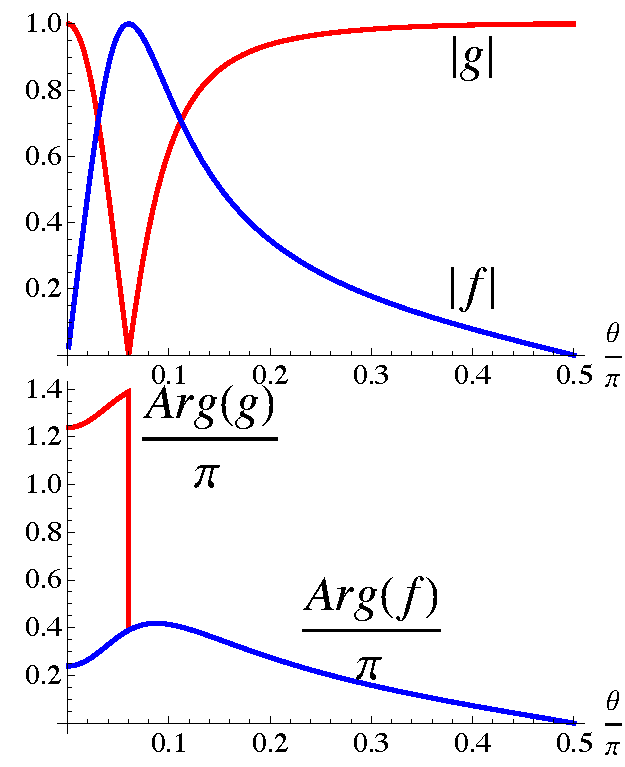
\includegraphics[width=\textwidth]{include/scatt.pdf}
\caption{ The magnitudes (upper panel) and the phases (lower panel) of the spin-flip 
amplitude $f$ and spin-conserving amplitude $g$ versus the incident angle $\theta$.
$E=0.1$eV, $E_F$=0.28eV. $|g|^2+|f|^2=1$. Arg($g$) and Arg($f$) 
are shifted upward by $\pi$ for clarity.}
\end{figure}
%%%%%%%%%%%%%%%%%%%%%%%%%%

\section{Interface Spectrum and Scattering Matrix from Lattice Green Function} 

We consider a simple lattice model for the M-TI junction.
The topological insulator is modeled by 
a tight binding Hamiltonian on cubic lattice,
\begin{eqnarray*}
&\mathscr{H}_R=\sum_{\kp,n}\left\{ 
\hat{\psi}_{\kp,n}^\dagger (b_1\hat{\Gamma}_0-i\frac{a_1}{2}\hat{\Gamma}_3)  \hat{\psi}_{\kp,n+1}+ h.c. \right. \\
&+\left. 
\hat{\psi}_{\kp,n}^\dagger\left[d(\kp)\hat{\Gamma}_0+a_2(\hat{\Gamma}_1\sin k_x +\hat{\Gamma}_2\sin k_y)\right] \hat{\psi}_{\kp,n} \right\} .
\end{eqnarray*}
Here $\hat{\psi}=(\psi_{+\uparrow},\psi_{+\downarrow},\psi_{-\uparrow},\psi_{-\downarrow})^\mathrm{T}$ is the annihilation operator, $d(\kp)=M-2b_1+2b_2(\cos k_x+\cos k_y-2)$ with $k$ measured in $1/a$. 
The cubic lattice consists of layers of square lattice stacked in the $z$ direction,
$n$ is the layer index, and $\kp$ is the momentum in the $xy$ plane.
The isotropic version of $\mathscr{H}_R$, with $a_1=a_2$, $b_1=b_2$, was 
studied by Qi et al as a minimal model for 3D topological insulators \cite{qi_field}.
To mimic Bi$_2$Se$_3$, we set the lattice spacing $a=5.2$\AA, which gives the correct unit cell volume, 
and $a_i=A_i/a$, $b_i=B_i/a^2$ for $i=1,2$. Although a crude caricature 
of the real material, $\mathscr{H}_R$ yields the correct gap size and surface dispersion, it also reduces to 
the continuum  $\mathbf{k\cdot p}$ Hamiltonian $\hat{H}_{TI}$ in the small $k$ limit, 
aside from the topologically trivial $\epsilon_0(\v{k})$ term.
 
%%%%%%%%%%%%%%%%%%%%%%%%%%
\begin{figure}
\center
%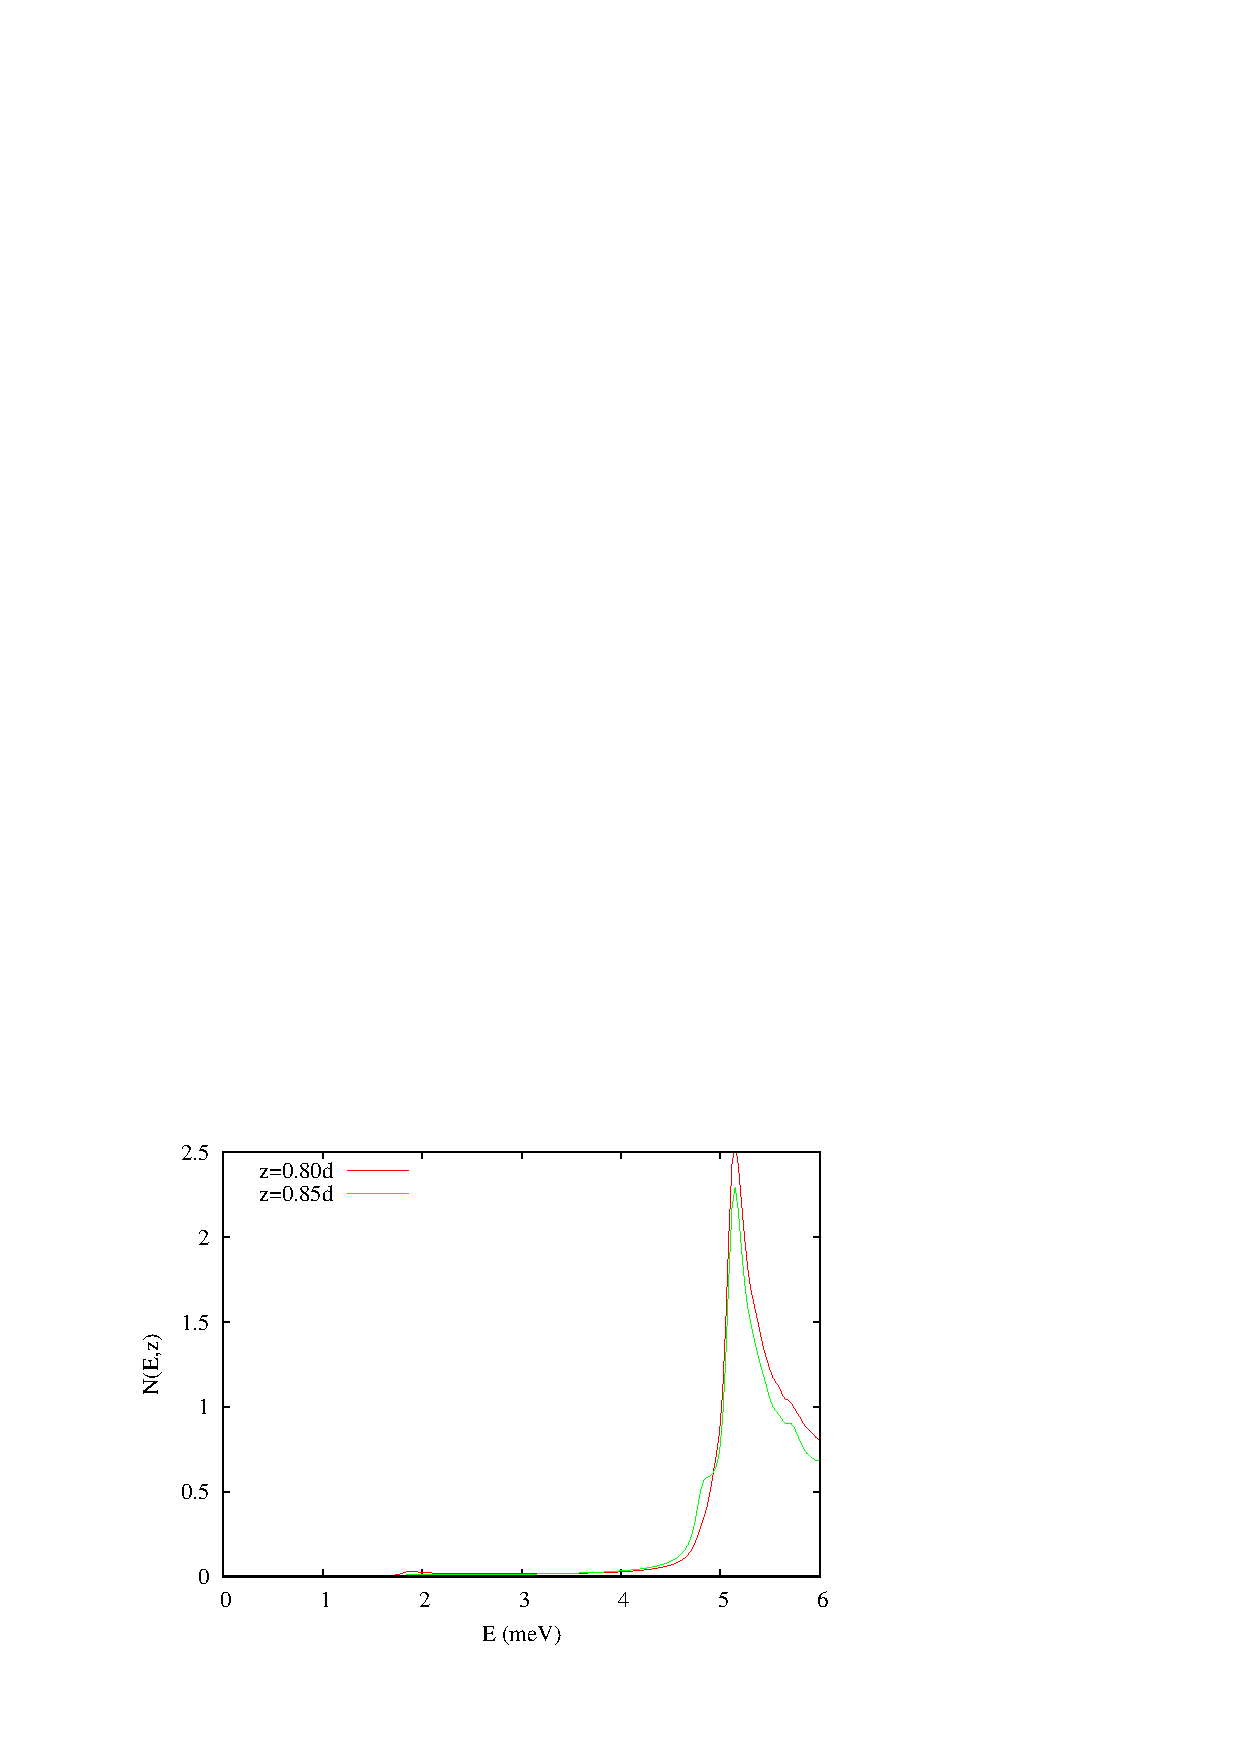
\includegraphics[width=3.4in]{dos.pdf}
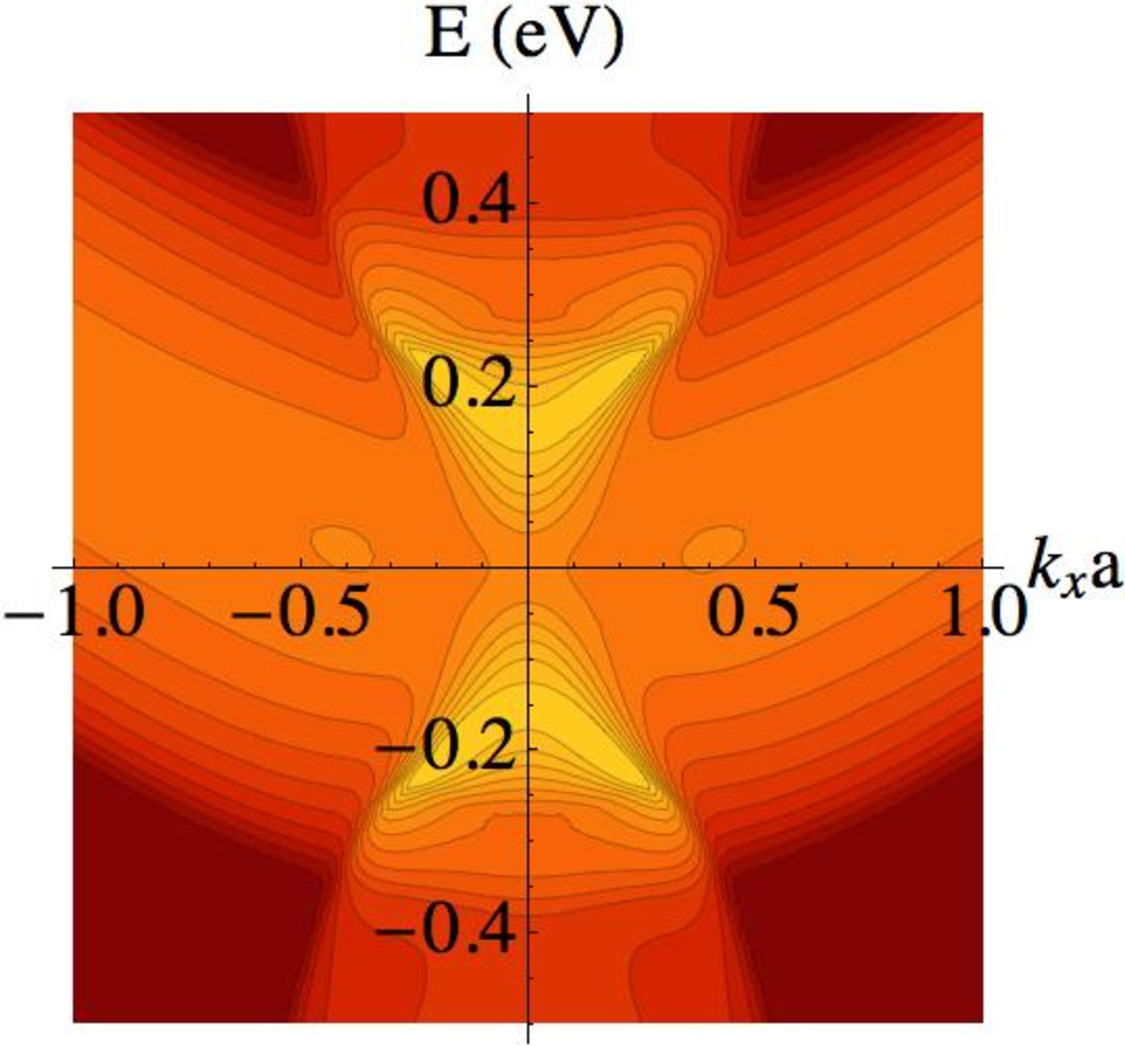
\includegraphics[width=.45\textwidth]{include/j1.pdf}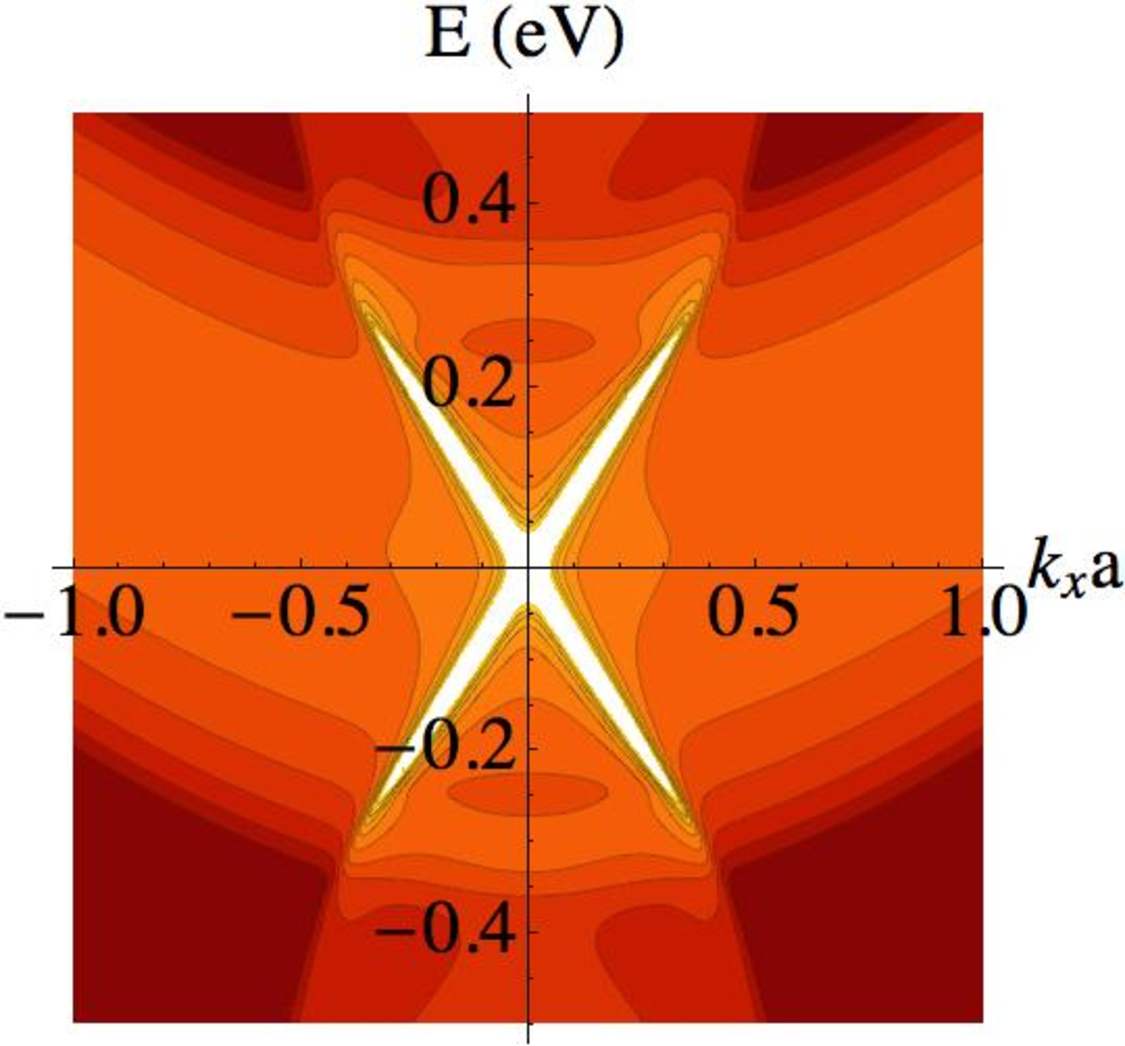
\includegraphics[width=.45\textwidth]{include/j2.pdf}
\caption{The spectral function $N(E,k_x,k_y=0)$ at the interface of metal and topological insulator. Left: 
good contact, $J=t_M$, showing the continuum of metal induced gap states. 
Right: poor contact with low transparency, $J=0.2t_M$, showing well 
defined Dirac spectrum as on the TI surface. $t_M=0.18eV$, $\mu_M=-4t_M$, $a$ is lattice spacing.}
\end{figure}
%%%%%%%%%%%%%%%%%%%%%%%%%%
 
As a generic model for metal, we consider a single band tight binding Hamiltonian on cubic lattice,
\[
\mathscr{H}_L=\sum_{\kp,n,\sigma}[h({\kp})  n_{\kp,n,\sigma}
- t_M \phi_{\kp,n,\sigma}^\dagger  \phi_{\kp,n+1,\sigma} + h.c.] 
\]
where $h(\kp)=-2t_M(\cos k_x+\cos k_y)-\mu_M$. 
The Fermi surface parameters of the metal can be varied by tuning $t_M$ and $\mu_M$.
The metal occupies the left half space, $n\leq 0$, and 
the TI occupies the right half space $n\geq 1$. The interface domain consists of layer $n=0,1$. 
The coupling between metal and TI is described by hopping,
\[
\mathscr{H}_{LR}=-\sum_{\kp,\ell,\sigma}J_{\ell}\psi^{\dagger}_{\kp,n=1,\ell,\sigma}\phi_{\kp,n=0,\sigma}+h.c.
\]
$J_{\ell}$ is the overlap integral between the $p$-orbital $\ell=\pm$ of TI and the $s$-like orbital of metal. For simplicity, we assume $J_{\ell}$ is independent of spin. Then, $J_{+}=-J_{-}=J$. $J$ can be tuned from weak to strong. Small $J$ mimics a large tunneling barrier between M and TI, 
and large $J$ (comparable to $t_M$ or $B_2$) describes a good contact. 

%%%%%%%%%%%%%%%%%%%%%%%%%%
\begin{figure}
\center
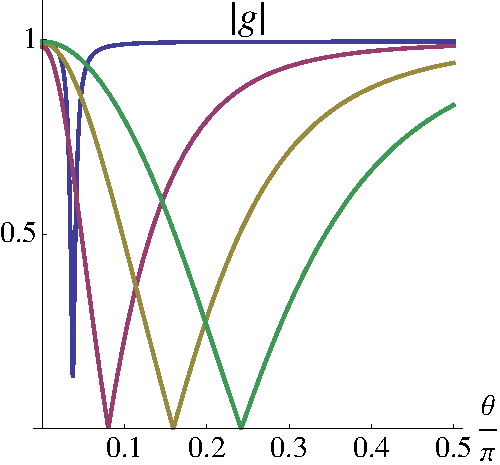
\includegraphics[width=.45 \textwidth]{include/la1.pdf}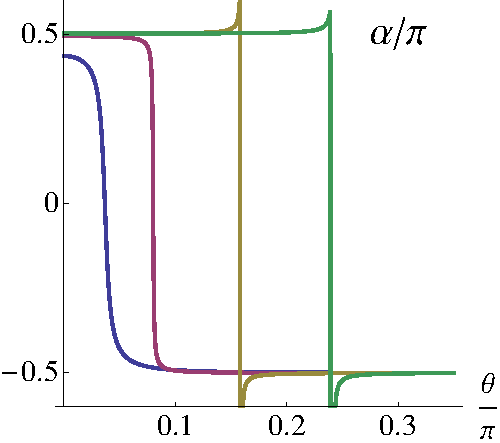
\includegraphics[width=.45 \textwidth]{include/la2.pdf}
\caption{The spin-conserving reflection amplitude $|g|$ and spin rotation angle 
$\alpha$ versus the incident angle $\theta$ for increasing contact transparency,
$J/t_M=0.25, 1, 1.5, 2$ (from left to right). $t_M=0.18eV$, $\mu_M=-4t_M$, $E=0.05$eV, $k_y=0$.
$|f|^2=1-|g|^2$. 
}
\end{figure}
%%%%%%%%%%%%%%%%%%%%%%%%%%

The lattice Green function of the composite system is computed via 
standard procedure by introducing the inter-layer transfer matrix 
and the method of interface Green function matching \cite{gf}. 
Fig. 4 shows two examples of the local spectral function 
(momentum-resolved density of states) at the interface,
\[ 
N(E,\kp)=-\sum_{n=0,1}\mathrm{Im Tr}\hat{\mathscr{G}}(E,\kp)_{n,n}, 
\]
where $\hat{\mathscr{G}}(E,\kp)_{n,n'}$ is 
the local Green function at the interface with $n,n'=0,1$, and  
the trace is over the spin and orbital space. 
In the tunneling (weak coupling, small $J$) limit, the interface spectrum includes 
a sharply defined Dirac cone as on the surface of TI. As $J$ is increased, 
the linearly dispersing mode becomes ill defined and eventually replaced 
by a continuum of metal induced gap states.

Once the lattice Green function is known for given incident $E$ and $k_{\parallel}$, 
the scattering (reflection) matrix can be constructed from $\hat{\mathscr{G}}$ by \cite{gf},
\[
\hat{S}(E,\kp)=\hat{\mathscr{G}}(E,\kp)_{0,0}g_M^{-1}(E,\kp)-\hat{1}
\]
where $g_M$ is the spin-degenerate bulk Green function of metal. Fig. 5 shows
the evolution of $|g(\theta)|$ and $\alpha(\theta)$ for increasing $J$, where 
a level broadening of $E/10$ is used. Most importantly,
we observe that the existence of a critical angel $\theta_c$, 
where complete spin-flip occurs and $\alpha$ jumps by $\pi$, is a robust phenomenon. 
It is independent of the details of the contact, the metal Fermi 
surface, or other high energy features in the band structure.

To understand the perfect spin flip, we first focus on 
the tunneling limit, $J\ll t_M$. In this limit, the local spectrum at layer $n=1$ as shown
in the right panel of Fig. 4 approaches
the TI surface spectrum, namely the helical Dirac cone. An incident up spin 
tunneling across the barrier will develop resonance with the helical mode, which is
a quasi-stationary state with long life time, if its 
momentum and energy satisfy $k_\parallel=E/A_2$. Moreover, it has to flip its spin, since 
only down spin can propagate in the $k_x$ direction (suppose $k_y=0$). 
The $\pi$ jump in the phase shift is also characteristic of the resonance. Indeed,
we have checked that precisely at $\theta_c$ the resonance criterion, $k_f\sin\theta_c=E/A_2$, 
is met.
We also varied $\mu_M$ for fixed $J$ and $t_M$, bigger $\mu_M$ 
yields a bigger Fermi surface and a smaller $\theta_c$. This is consistent with 
the resonance criterion above.

As $J$ is increased, the width of the resonance grows and eventually it is replaced by a 
broad peak (dip) in $|f|$ ($|g|$), but the vanishing of $|g|$ and $\pi$
shift in $\alpha$ at $\theta_c$ persist to good contacts,
even though in this limit the interface is flooded by MIGS (left panel of Fig. 4) 
and bears little resemblance to the Dirac spectrum.
With all other parameters held fixed, $\theta_c$ increases with $J$. Qualitatively,
coupling to TI renormalizes the metal spectrum near the interface, producing a smaller effective $k_f$ (hence a larger $\theta_c$) compared to its bulk value. 
It is remarkable that perfect spin flip at the critical angle persists all
the way from poor to good contacts. Indeed, the main features observed here for
for good contacts using the lattice model 
agree well with the results obtained in previous section by wave function matching. 

\section{Discussions}

We now discuss the experimental implications of our results. The M-TI interface spectrum can be measured by 
ARPES (or scanning tunneling microscope) experiments on metal film coated on a topological insulator.
Our results also suggest that a topological insulator can serve as a perfect mirror to flip the 
electron spin in metal. Such spin-active scattering at the M-TI interface may be 
exploited to make novel spintronic devices. The magnitude of $g$ or $f$
can be measured by attaching two ferromagnetic leads to a piece of metal in contact with TI, 
forming a multi-terminal device. 
One of the ferromagnetic leads produces spin-polarized electrons incident on the M-TI interface at some angle, while 
the other lead detects the polarization of reflected electron, as in a
giant magneto-resistance junction. The spin rotation angle $\alpha$ can be measured 
indirectly by comparing the predicted current-voltage characteristics of M-TI-M 
or Superconductor-TI-Superconductor junctions, which are sensitive the phase shift $\alpha$. It can also be inferred from 
the spin transport in a TI-M-TI sandwich, as discussed for QSH insulator in Ref. \cite{yokoyama09}.
Detailed calculations of the transport properties of these structured,
using the scattering matrix obtained here, will be subjects of future work.


\chapter{Superconducting Proximity Effect}
In the first chapter we described the topological insulator and it's novel features. We also described the exotic $p-$wave superconductor and along with the topological insulator in proximity to an $s-$wave superconductor. We showed that these systems are topological in the sense that there exist with gap-less modes localized near certain boundaries. These edge states have linear dispersions.

In this chapter we focus on the superconductor-topological insulator heterostructure. This structure is predicted by Fu and Kane to be a host to a Majorana fermion under certain conditions. Our focus is not on the phenomenological properties of the Majorana regime, but rather to understand the behavior of the system in a more realistic fashion. We set up the Bogoliubov-de Gennes model for a TI and a superconductor to calculate the eigensystem in a recursive, self-consistent manner. The eigen energies and wave functions provide the framework we need to calculate several quantitative properties. These include order parameter, $\Delta(z)$, spatially resolved spectral function, $A(z,k,\epsilon)$, local density of states, $N(z,\epsilon)$. In addition we also find singlet ($F_{\uparrow \downarrow}(k,z)$) and triplet ($F_{\uparrow \uparrow}(k,z)$ $F_{\downarrow \downarrow}(k,z)$) pairing correlations. We show that the energy spectrum does indeed host sub-gap states as predicted by Fu-Kane with renormalized parameters. We also find triplet correlations, exhibiting $p_x+ip_y$ behavior, consistent with previous studies of a similar system.

\section{Introduction}
Fu and Kane showed that 
at the interface between a three-dimensional topological band insulator  (TI) and an 
$s$-wave superconductor (S) forms a remarkable two-dimensional non-Abelian superconductor \cite{f-k}.
It hosts Majorana zero modes at vortex cores, as in a 
$p_x+ip_y$ superconductor \cite{r-g}, but respects time-reversal symmetry. 
As argued in Ref. \cite{f-k}, the presence of superconductor induces a pairing interaction
between the helical Dirac fermions at the surface of the topological insulator,
and gaps out the surface spectrum. Then, the interface can be modeled elegantly by 
 a simple matrix Hamiltonian in Nambu space (we follow the convention of Ref. \cite{qi-zhang}),
\begin{equation}
H_{FK}(\mathbf{k})=\left(
\begin{array}{cc}
h_s(\mathbf{k})  &  i\sigma_y  \Delta_s \\
-i\sigma_y \Delta_s^*  &   -h_s^*(-\mathbf{k})
\end{array}\label{fkmodel}
\right),
\end{equation}
where $\mathbf{k}=(k_x,k_y)$ is the two-dimensional momentum in
the interface plane, $\sigma_i$ are the Pauli matrices,
$h_s(\mathbf{k})$ is the surface Hamiltonian
for the topological insulator describing the helical Dirac fermions \cite{qi-zhang,rmp},
\begin{equation}
h_s(\mathbf{k})=-\mu_s + v_s (\sigma_xk_y-\sigma_y k_x).
\end{equation}
Fu and Kane also proposed to use S-TI proximity structures to
generate and manipulate Majorana fermions which obey non-Abelian 
statistics and are potentially useful for fault tolerant quantum 
computation \cite{f-k}. 
This proposal and a few others that followed based on 
superconductor-semiconductor heterostructures \cite{roman,maryland,jason,mao1,mao2} have revived
the interest in superconducting proximity effect involving insulating/semiconducting 
materials with spin-orbit coupling. More complex S-TI proximity structures
with ferromagnets \cite{yu,jacF} or unconventional superconductors \cite{jacU} 
have been investigated.

Experiments are beginning to realize various S-TI proximity structures \cite{sca,march1,march2}.
In light of these developments, it is desirable to
understand to what extent the effective model $H_{FK}$ holds,
and what are the values of $(\Delta_s,\mu_s,v_s)$ for given materials. 
Answering these questions is crucial for future experiments designed to probe
and manipulate Majorana fermions. As a first step in this
direction, Stanescu et al considered a microscopic lattice model
for the TI-S interface \cite{stan}. In this model, TI and S are described by a tight binding 
Hamiltonian defined on the diamond and hexagonal lattice respectively.
The two materials are coupled by tunneling term in the Hamiltonian. 
These authors found that 
for small $\mathbf{k}$, $H_{FK}(\mathbf{k})$ is valid but its parameters are 
significantly renormalized by the presence of the superconductor. 
This is supported by leading order 
perturbation theory in the weak coupling (tunneling) limit. They also
discussed the induced $p$-wave correlation within the framework of
perturbation theory. The $p$-wave correlation has also been noted in 
an analogous proximity structure in two dimension between
a quantum spin Hall insulator and a superconductor \cite{ann}.


In this work, we consider S-TI proximity structures where 
S and TI are {\it strongly} coupled to each other, 
rather than being separated by a tunneling barrier.
This is the desired, presumably the optimal, configuration to realize the Fu-Kane
proposal, e.g. to achieve maximum value of $\Delta_s$ in $H_{FK}$ for given
superconductor. 
In the strong coupling limit, 
the modification of superconductivity by the TI becomes important.
This includes the suppression of the superconducting order parameter,
the induction of triplet pair correlations by spin-active scattering
at the interface, and the formation of interface states below the bulk superconducting gap.
In order to accurately answer questions raised in the preceding paragraph
for strongly coupled S-TI structures, one has to self-consistently 
determine the spatial profile of 
the order parameter near the interface.

Our work is also motivated by recent experimental discovery that Copper-doped 
topological insulator Cu$_x$Bi$_2$Se$_3$
becomes superconducting at a few Kelvins \cite{cu1,cu2,ando}. It 
seems possible then to combine such superconductors with topological insulator 
Bi$_2$Se$_3$ to achieve strong proximity coupling. 
% Using Bi$_2$Se$_3$ and Cu$_x$Bi$_2$Se$_3$ as one of the examples,
We set up microscopic, continuum models for the S-TI structures and solve the result 
Bogoliubov-de Gennes (BdG) equation numerically.
We first compute the superconducting order 
parameter as a function of the distance
away from the interface.
We then verify the validity of the Fu-Kane effective model
and extract its parameters from the low energy sector of the energy
spectrum. The emergence
of $H_{FK}$ will be viewed as the result of the ``inverse proximity effect", namely
strong modification of superconductivity by the presence of TI.
This is in contrast to the previous viewpoint of
pairing between surface Dirac fermions, which is a more proper description
in the tunneling limit.
The spectral weight of these low energy modes (with energy below the bulk superconducting gap) 
are shown explicitly to peak near the interface but penetrate well
into the superconductor.
We will also show analytically that the induced triplet pair
correlations are of $p_x\pm ip_y$ orbital symmetry, and systematically
study their spatial and momentum dependence.
Our results connect the phenomenological theory of Fu and Kane \cite{f-k}
to real materials. Our results for continuum models and strong coupling 
limit are also complementary to the results of Stanescu et al \cite{stan}
for lattice models and tunneling limit.

In what follows, we first outline the formulation of the problem and 
then present the main results. Technical details on numerically solving
the BdG equation are relegated to the appendix.

\section{Model and Basic Equations}

The band gaps of topological insulators are much larger than the superconducting
gap of all  weak coupling $s$-wave superconductors. 
For the purpose of studying the proximity
effect between such superconductors and topological insulators, it is
sufficient to describe the topological insulator using the 
low energy effective $\mathbf{k}\cdot \mathbf{p}$ Hamiltonian. Following
Zhang et al \cite{zhang}, we model Bi$_2$Se$_3$ by 
\begin{eqnarray}
H_{TI}({\bf k})=
\left( \begin{array}{cccc}
M({\bf k}) & 0 & A_1 k_z  & A_2 k_{-} \\
0 &M({\bf k})& A_2 k_+ & -A_1 k_z \\
 A_1 k_z  & A_2 k_{-} &-M({\bf k}) & 0 \\
A_2 k_+ & -A_1 k_z &0 & -M({\bf k}) \\
 \end{array} \right)-\mu \hat{I}.
 \end{eqnarray}
Here $k_{\pm}=k_x \pm i k_y $, 
$M({\bf k})=M-B_1 k_z ^2 - B_2 (k_x^2 + k_y^2)$, and $\hat{I}$ is $4\times 4$
unit matrix. The numerical values of 
the parameters are obtained from first principle calculations \cite{zhang,band}, $M=0.28$ eV,
$A_1=2.2$ eV\AA, $A_2=4.1$ eV\AA, $B_1=10$ eV\AA$^2$, $B_2=56.6 $ eV\AA$^2$.
We work in basis $\{\ket{1\uparrow}, \ket{1\downarrow},\ket{2\uparrow},\ket{2\downarrow} \}$,
where 1 (2) labels the $P1_z^+$ ($P2_z^+$) orbital \cite{zhang}. Note that
we have neglected the unimportant diagonal term $\epsilon_0({\bf k})$ in Ref. \cite{zhang} which 
only slightly modifies the overall curvature of the band dispersion. We also
keep the chemical potential $\mu$ as a tuning parameter.

We consider a simple model of superconductor derived from a metallic
state obtained by turning off the spin-orbit coupling ($A_1=A_2=0$) in
$H_{TI}$ and tuning the Fermi level well into the conduction band \cite{zhao}. The metal
Hamiltonian
\begin{eqnarray}
H_{M}({\bf k})=\mathrm{diag} [M({\bf k}), M({\bf k}), -M({\bf k}), -M({\bf k})]-E_f \hat{I},
\end{eqnarray}
with  $E_f>M$. 
This mimics electron-doping the topological insulator \cite{cu2} 
or equivalently electrochemically
shifting its chemical potential by applying a gate voltage \cite{gate}.
As shown in Fig. \ref{setup}, 
the valence band (band 1 with dispersion $M({\bf k})-E_f$) is well below the Fermi level and remains inert as far as 
superconductivity is concerned.  Next, within the framework of Bardeen-Cooper-Schrieffer
theory, we assume attractive interaction between
the electrons in the conduction band (band 2) near the Fermi surface described by the reduced
 Hamiltonian,
\begin{equation}
H_{int}=\sum_{\bf k} \psi^\dagger_{2\uparrow}({\bf k})\psi^\dagger_{2\downarrow}(-{\bf k})\Delta + h.c.
\end{equation}
Here $\Delta$ is the 
superconducting order parameter, $\psi^\dagger_{l\sigma}$ is the electron creation operator for orbital $\l=1,2$ and
spin $\sigma=\uparrow,\downarrow$. The superconductor is then described by 
\begin{equation}
H_S=\sum_{{\bf k},l,\sigma}\psi^\dagger_{l\sigma}({\bf k})H_M({\bf k})_{l\sigma,l\sigma}\psi_{l\sigma}({\bf k})+H_{int}.
\end{equation}
Note that $H_S$ and $H_{TI}$ are in the same 
basis.

This model can serve as a generic model for $s$-wave superconductors with negligible
spin-orbital coupling. Whether it can actually describe the superconductor Cu$_x$Bi$_2$Se$_3$
has to be settled by future experiments.
The transition temperature of Cu$_x$Bi$_2$Se$_3$ 
at optimal doping $x=0.12$ is $T_c=3.8$K, which corresponds to a zero 
temperature superconducting gap $\Delta\sim$0.6meV \cite{cu1,cu2,ando}. The Fermi level is 0.25eV 
above the bottom of the conduction band, and the Fermi wave vector $k_f\sim 0.12$\AA$^{-1}$.
The pairing symmetry of Cu$_x$Bi$_2$Se$_3$ is to our best knowledge is unknown at present (it appears
to be fully gapped from the specific heat measurement \cite{ando} and might be a 
topological superconductor \cite{cu2}). 
If it turns out to be a conventional $s$-wave superconductor, its mains 
features will be captured by $H_S$ above with suitable choice of $E_f$ and $\Delta$.

%%%%%%%%%%%%%%%%%%%%%%%%%%
\begin{figure}
\center
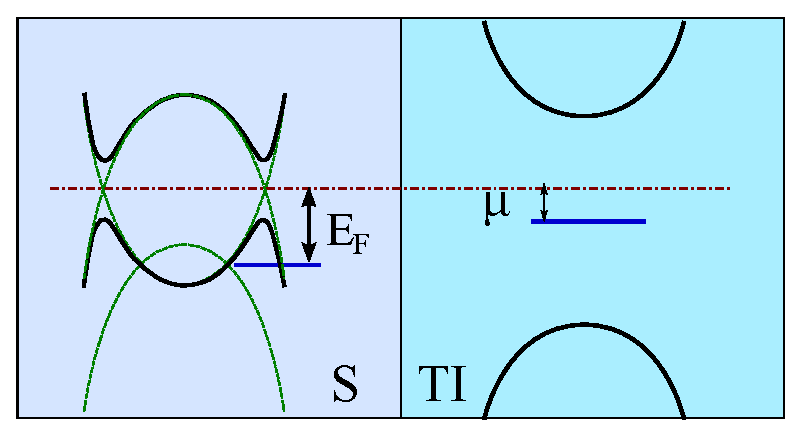
\includegraphics[width=\textwidth]{include/setup.eps}
\caption{Schematic (not to scale) band diagrams  in a superconductor-topological insulator (S-TI) proximity
structure. $E_f$ is the Fermi energy of the metal described by $H_M$ measured from the band crossing point. $\mu$ is
the chemical potential of TI measured from the band gap center. The superconducting gap
is much smaller than the band gap of TI.
}\label{setup}
\end{figure}
%%%%%%%%%%%%%%%%%%%%%%%%%%

Now consider a proximity structure consisting 
of a superconductor at $z<d$ and a topological insulator at $z>d$ (Fig. \ref{setup}).
The interface at $z=d$ is assumed to be specular, so the momentum $\mathbf{k_\parallel}=(k_x,k_y)$ 
parallel to the interface is conserved. The Hamiltonian for the whole system 
\begin{align}
\mathcal{H} = &\int d \mathbf{k}_\parallel dz
\Bigl\{ \sum_{\sigma} \psi^{\dagger}_{1 \sigma}(\mathbf{k}_\parallel,z)[h_0 - \mu(z)] \psi^{\dagger}_{1 \sigma}(\mathbf{k}_\parallel,z) 
 \nonumber \\
&- \sum_{\sigma} \psi^{\dagger}_{2 \sigma}(\mathbf{k}_\parallel,z)[h_0 + \mu(z)] \psi^{\dagger}_{2 \sigma}(\mathbf{k}_\parallel,z)\nonumber \\
&+\Delta(z)  \psi^{\dagger}_{2 \uparrow}(\mathbf{k}_\parallel,z) \psi^{\dagger}_{2 \downarrow} (-\mathbf{k}_\parallel,z)+h.c.\nonumber \\
&+A_1(z) [\psi^{\dagger}_{1 \uparrow} (-\idz) \psi_{2 \uparrow} 
+\psi^{\dagger}_{1 \downarrow} (\idz) \psi_{2 \downarrow}+h.c.]  \nonumber\\
&+A_2(z)
[\psi^{\dagger}_{1 \uparrow} \ki \psi_{2 \downarrow} +\psi^{\dagger}_{1 \downarrow} \kp \psi_{2 \uparrow} +h.c.]
\Bigr \}. \label{hbH}
\end{align}
Here $h_0(\mathbf{k}_\parallel, \partial_z)=M -B_1 \partial_z^2 -B_2 k_\parallel^2$, $\mu(z)$ and $A_i(z)$
are piece-wise constant, 
\begin{align}
\mu(z)&=E_f\theta(d-z)+\mu\theta(z-d),\\
A_i(z)&=A_i\theta(z-d),\;\;i=1,2
\end{align}
in terms of the step function $\theta$. The order parameter obeys the gap equation
\begin{equation}
\Delta(z) = g(z) \int d \mathbf{k}_\parallel \langle {\psi_{2 \uparrow}(\mathbf{k}_\parallel,z) \psi_{2 \downarrow}(-\mathbf{k}_\parallel,z) }\rangle. \label{gapE}
\end{equation}
We assume $g(z)=g\theta(d-z)$, the coupling constant $g$ determines the bulk gap.

To self-consistently solve Eq. \eqref{hbH} and \eqref{gapE}, we introduce
Bogoliubov transformation
\begin{equation}
 \psi_{l \sigma}(\mathbf{k}_\parallel,z) = \sum_n  u_{n,l \sigma} (\kperp, z) \gamma_{n,\kperp} + v^\ast_{n,l \sigma} (\kperp, z) \gamma_{n,\kperp}^\dagger
\end{equation}
to diagonalize $\mathcal{H}$ as
\begin{equation}
\mathcal{H} = E_g + \int d \kperp\sum_n \epsilon_n(k_\parallel) \gamma_{n,\kperp}^\dagger \gamma_{n,\kperp} ,
\end{equation}
where $E_g$ is the ground state energy, and $\gamma_{n,\kperp}^\dagger$
is the creation operator of Bogoliubov quasiparticles with energy $\epsilon_n(k_\parallel)$.
The wave function $u$ and $v$ satisfy the following Bogoliubov-de Gennes (BdG) equation,
\begin{equation}
\hat{H}_{B}(\mathbf{k}_\parallel,z) \hat{\phi}_n(\mathbf{k}_\parallel,z)=\epsilon_n(k_\parallel)\hat{\phi}_n (\mathbf{k}_\parallel,z).
\label{bdgsimp}
\end{equation}
Here, the BdG Hamiltonian
\begin{equation}
\hat{H}_{B}=\left( \begin{array}{cccc}
h_0 -\mu  & \mathbf{d} \cdot \boldsymbol{\sigma}&0&0\\ 
 \mathbf{d} \cdot \boldsymbol{\sigma} &-h_0 -\mu &0&-\Delta\, i\sigma_y\\ 
0 &0& \mu -h_0 & \mathbf{d} \cdot \boldsymbol{\sigma}^* \\
0 &\Delta^{\ast} \, i\sigma_y & \mathbf{d} \cdot \boldsymbol{\sigma}^* & \mu+h_0\\ 
 \end{array} \right), \label{bdgH} 
\end{equation}
and the wave function (dropping the arguments)
\begin{equation}
\hat{\phi}_n=(u_{n,1\uparrow}, u_{n,1\downarrow}, u_{n,2\uparrow}, u_{n,2\downarrow}, 
v_{n,1\uparrow}, v_{n,1\downarrow}, v_{n,2\uparrow}, v_{n,2\downarrow})^\mathrm{T}.
\end{equation}
The vector $\mathbf{d}(\mathbf{k}_\parallel,z)$ is defined as
\begin{equation}
d_x=A_1(z)k_x,\,\, d_y=A_1(z)k_y,\,\, d_z=A_2(z)(-i\partial_z).
\end{equation} 
Other quantities such as $h_0(\mathbf{k}_\parallel,z)$, $\mu(z)$, and $\Delta(z)$ are 
defined above.
In terms of the wave functions, the zero temperature gap equation becomes
\begin{equation}
\Delta(z) = g(z) \int d \mathbf{k}_\parallel \sum_n' u_{n,2 \uparrow}(\mathbf{k}_\parallel,z) v^*_{n,2\downarrow}(-\mathbf{k}_\parallel,z) ,
\end{equation}
where the summation denoted by prime is restricted to $0<\epsilon_n<\omega_D$ with 
$\omega_D$ being the Debye frequency.


We will exploit a particular symmetry of the BdG Hamiltonian to simplify 
calculations. Define the polar angle $\varphi_k$ for the in-plane wave vector $\kperp$, 
\begin{equation}
k_x+ik_y=k_{\parallel}e^{i\varphi_k}.
\end{equation}
Then the BdG Hamiltonian for arbitrary $(k_x,k_y)$ is
related to that for $(k_x=k_\parallel,k_y=0)$ by unitary transformation 
\begin{equation}
\hat{U}^\dagger(\kperp) \hat{H}_{B}(k_x,k_y) \hat{U}(\kperp) = \hat{H}_{B}(k_\parallel,0).
\label{symm}
\end{equation}
Here $U$ is a 
block diagonal matrix,
\begin{equation}
U(\kperp)=\mathrm{diag}[e^{-i\sigma_z\frac{\varphi_k}{2}}, e^{-i\sigma_z\frac{\varphi_k}{2}}, e^{i\sigma_z\frac{\varphi_k}{2}},e^{i\sigma_z\frac{\varphi_k}{2}} ]. \label{unit}
\end{equation}
Thus, the eigen energy $\epsilon_n$ only depends on the magnitude of $\kperp$.
Once the wave function for $\varphi_k=0$ is known, the wave function for $\varphi_k\in (0,2\pi)$
can be obtained by simple unitary transformation.

We solve the matrix differential equation \eqref{bdgsimp} by conserving it into an algebraic equation, 
following the treatment of superconductor-ferromagnet structure by 
Halterman and Valls \cite{h-v}. The whole S-TI proximity structure is assumed to have 
finite dimension $L$ in the $z$
direction. The superconductor occupies the region $0<z<d$,
while the topological insulator occupies $d<z<L$. Hard wall boundary conditions are enforced at the end points, 
$z=0$ and $z=L$.  
The exact boundary conditions at the end points only affect the local physics there, provided 
that the boundaries are sufficiently far away from the S-TI interface. We expand the wave function
and order parameter in Fourier series \cite{h-v},
\begin{align}
u_{n,l\sigma}(z) &= \sum_m u_{nm}^{l \sigma}\,\phi_m(z),\label{uexp}\\ 
v_{n,l\sigma}(z) &= \sum_m v_{nm}^{l \sigma}\, \phi_m(z),\\
\quad \Delta(z) &= \sum_m \Delta_{m}\, \phi_m(z) , \label{Dexp}\\
\phi_m(z)&=\sqrt{2/L}\sin(k_m z).
\end{align}
The integer $m=1,2,...,N$ labels the quantized longitudinal (along $z$) momentum $k_m=m\pi/L$. 
The cutoff $N$ is chosen as \cite{s-v}
\begin{equation}
B_1k^2_N=M+E_f+\omega_D. \label{eq-N}
\end{equation}
By expansion Eq. \eqref{uexp}-\eqref{Dexp}, the BdG equation
becomes an $8N \times 8N$ matrix equation. With a reasonable guess of the order parameter profile, 
the eigen energies and eigen wave functions are obtained by solving the matrix eigen value problem.
Then a new order parameter profile is computed from the gap equation. The procedure is iterated
until convergence is achieved.  Relevant technical details can be found
in the Fourier calculations section. 

To analyze the spectrum of the system, it is convenient to define the retarded Green's function
\begin{equation}
G^R_{l\sigma}(\mathbf{k}_\parallel,z,t)=-i\theta(t)\langle \{\psi_{l\sigma}(\mathbf{k}_\parallel,z,t),
\psi^\dagger_{l\sigma}(\mathbf{k}_\parallel,z,0)\}\rangle
\end{equation}
where the time-dependent field operators are in Heisenberg picture. 
For given $\kperp$ and $z$, the spectral functions 
are defined as
\begin{align}
&N_{l\sigma}(\mathbf{k}_\parallel,z,\omega)= -\mathrm{Im}G^R_{l\sigma}(\mathbf{k}_\parallel,z,\omega), \\
&N(\mathbf{k}_\parallel,z,\omega)=\sum_{l\sigma}N_{l\sigma}(\mathbf{k}_\parallel,z,\omega).
\end{align}
In terms of the wave functions and eigen energies, 
\begin{equation}
N_{l\sigma}(\mathbf{k}_\parallel,z,\omega>0)=\sum_n|u_{n,l\sigma}(\mathbf{k}_\parallel,z)|^2\delta(\omega-\epsilon_n). 
\end{equation}
We also introduce the equal-time pair correlation functions
for the conduction electrons 
\begin{equation}
F_{\alpha\beta}(\mathbf{k}_\parallel,z)=\langle \psi_{2\alpha}(\mathbf{k}_\parallel,z) \psi_{2\beta}(-\mathbf{k}_\parallel,z)\rangle.\label{pair-corr}
\end{equation}
For example, at zero temperature we have
\begin{align}
F_{\uparrow\uparrow}(\mathbf{k}_\parallel,z)=\sum'_n u_{n,2\uparrow}(\mathbf{k}_\parallel,z)
v^*_{n,2\uparrow}(-\mathbf{k}_\parallel,z),\\
F_{\downarrow\downarrow}(\mathbf{k}_\parallel,z)=\sum'_n u_{n,2\downarrow}(\mathbf{k}_\parallel,z)
v^*_{n,2\downarrow}(-\mathbf{k}_\parallel,z).
\end{align}
Triplet components of $F$ will be induced near the S-TI interface by spin-active
scattering \cite{zhao}.

%\appendix*
\section{Fourier Expansion}
We follow the numerical scheme of Halterman and Valls to solve 
the matrix BdG equation \cite{h-v}. The wave functions and the order parameter
are expanded in the orthonormal basis $\{\phi_m(z)\}$, with $m=1,...,N$. For example,
function $u_{n,1\uparrow}(z)$ is represented by $N$ numbers,
\begin{align*}
(u^{1\uparrow}_{n,1},u^{1\uparrow}_{n,2},...u^{1\uparrow}_{n,m}...,u^{1\uparrow}_{n,N}).
\end{align*}
Accordingly, each term in $\hat{H}_{B}$ is represented
by a $N\times N$ matrix with the matrix elements given by
\begin{align*}
h_0(\kperp,\partial_z) &\rightarrow \delta_{mm'}(M - B_1 k_m^2 - B_2 k_\parallel^2) \\
U(z) &\rightarrow E_f E_{mm'} + \mu F_{mm'} \\
 A_2(z) \partial_z &\rightarrow A_2 G_{mm'}\\
 A_1(z) k_\pm &\rightarrow A_z k_\pm F_{mm'} \\
 \Delta &\rightarrow D_{mm'}\equiv \sum_{m''}J_{m,m',m''}\Delta_{m''}
\end{align*}
where 
\begin{align*}
E_{mm'}&=\int_0^{d} \phi_m(z) \, \phi_{m'}(z) dz \\
F_{mm'}&=\int_d^{L} \phi_m(z) \, \phi_{m'}(z) dz \\
G_{mm'}&=\int_d^{L} \phi_m(z) \partial_z \phi_{m'}(z) dz\\
J_{m,m',m''}&=\int_0^{d} \phi_m(z) \, \phi_{m'}(z) \, \phi_{m''}(z) dz
\end{align*}
These integrals can be evaluated analytically. Then the BdG equation becomes
an $8N\times 8N$ matrix equation. The gap equation can be rewritten as
\[
\Delta_{m}=g\int d\kperp \sum'_n \sum_{m',m''} J_{m,m',m''}
u^{2\uparrow}_{nm'}(\kperp)v^{2\downarrow}_{nm''}(-\kperp)^* 
\]
The integral over $\kperp$ is first simplified to an integral over $k_\parallel$
by the symmetry Eq. \eqref{symm} and then evaluated numerically with high 
momentum cutoff 
$\sqrt{(E_F+\omega_D+M)/B_2}$.


\section{The Order Parameter}

%%%%%%%%%%%%%%%%%%%%%%%%%%
\begin{figure}
\center
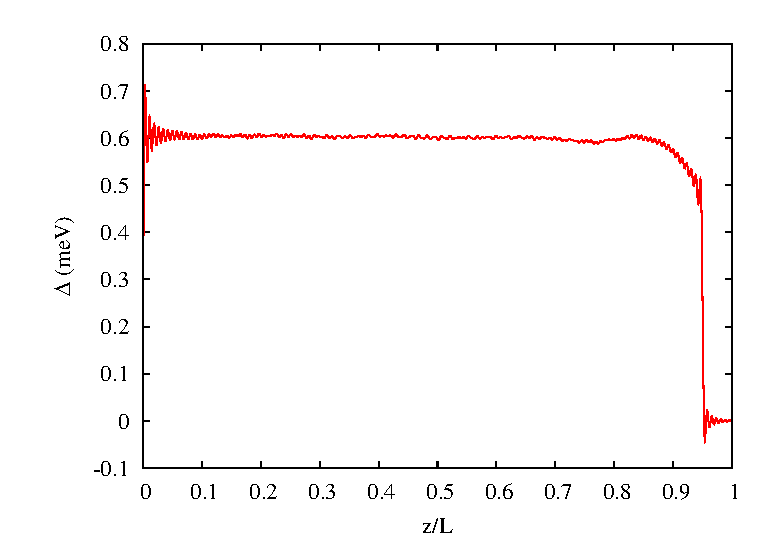
\includegraphics[width=\textwidth]{include/delta-cu.eps}
\caption{The superconducting order parameter $\Delta(z)$ near an S-TI interface at $
z=d=0.95L$. The superconductor occupies $0<z<d$, and topological insulator occupies $d<z<L$. 
$L=300$ nm, $\mu$=0, the bulk gap $\Delta_0=$0.6meV. }\label{delta-cu}
\end{figure}
%%%%%%%%%%%%%%%%%%%%%%%%%%

First we present the spatial profile of the superconducting order parameter $\Delta(z)$
after the convergence is achieved. In all following calculations, $E_f$ is fixed at 0.4eV, 
which is modeled after optimally doped Cu$_x$Bi$_2$Se$_3$ \cite{cu2}. And the Debye frequency
is set as $\omega_D=0.1E_f$ \cite{h-v}.
%
Fig. \ref{delta-cu} shows an example with $\mu=0$, $L=300$nm, $d=0.95L$, and
a bulk gap of 0.6meV as found in Cu$_x$Bi$_2$Se$_3$. 
%
Going from the superconductor into the topological insulator,
$\Delta$ first gets suppressed as the interface is approached before it
drops to zero inside TI. The suppression is roughly 20\% at the interface.
Note that the fine wiggles of $\Delta$ in the simulation results 
are due to the finite momentum cutoff of 
the longitudinal momentum $k_m$. As previously discussed by 
Stojkovic and Valls \cite{s-v}, the number of oscillations is $\sim N/2$, and the 
oscillation amplitude vanishes in the bulk as $N$ is increased. 
In this case, $N$ is chosen to be
258 according to Eq. \eqref{eq-N}. So the matrix to be diagonalized is 2064 by 2064.

Fig. \ref{delta-24} show the result for $\mu=0$, $d=0.9L$, and 
a superconductor with bulk gap $\Delta_0\sim 2.4$meV. Since the coherence length
is much smaller than the previous example, it is sufficient to consider 
$L=160$nm, and correspondingly $N=138$. 
The order parameter profile  
depends weakly on $\mu$, as shown in Fig. \ref{delta-chem} for a superconductor
with bulk gap $\sim 5.2$meV. 
From these examples, one observes that the length scale over which $\Delta$ is 
significantly suppressed does {\it not} scale with $\xi_0$, the zero temperature
coherence length of the superconductor. Rather it stays roughly the same, 
on the order of $30$nm, as $\xi_0$ is varied over one decade from Fig. \ref{delta-cu}
to Fig. \ref{delta-chem} (note the horizontal axis is $z/L$). 
This is not very surprising since $\xi_0$ is not the only length scale at play here.
The interface represents a strong (as compared to $\Delta_0$) perturbation that 
significantly distorts the bulk wave functions.
The self-consistent microscopic BdG approach provides a reliable way to
capture the details of $\Delta(z)$ near the interface.


%%%%%%%%%%%%%%%%%%%%%%%%%%
\begin{figure}
\center
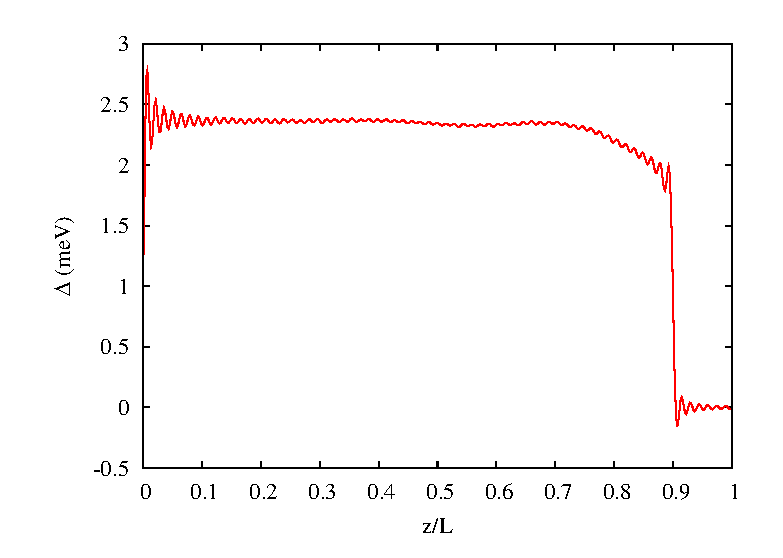
\includegraphics[width=\textwidth]{include/dt.eps}
\caption{The order parameter $\Delta(z)$ near an S-TI interface at $
z=d=0.9L$. $L=160$ nm, $\mu$=0, $\Delta_0\sim 2.4$meV.}
\label{delta-24}
\end{figure}
%%%%%%%%%%%%%%%%%%%%%%%%%%


%%%%%%%%%%%%%%%%%%%%%%%%%%
\begin{figure}
\center
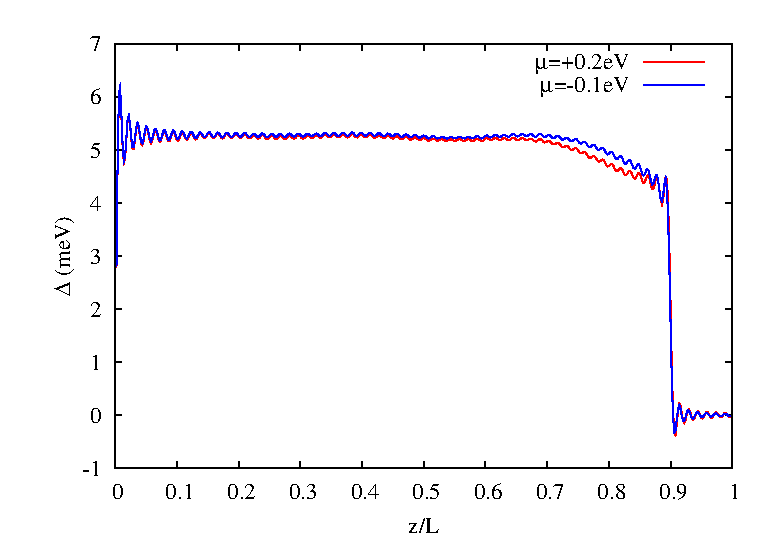
\includegraphics[width=\textwidth]{include/dtchemi.eps}
\caption{The order parameter profile for two different chemical potentials of
the topological insulator, $\mu=-0.1$eV and $\mu=0.2$eV. $L=160$nm,  
$\Delta_0\sim 5.2$meV. }\label{delta-chem}
\end{figure}
%%%%%%%%%%%%%%%%%%%%%%%%%%

It is illuminating to compare the proximity effect in S-TI
structure with that in S-F structure \cite{toku}, where F stands for 
a ferromagnetic insulator. 
The presence of F breaks time-reversal and spin rotation symmetry and 
significantly suppresses the order parameter. The suppression is
sensitive to the spin mixing angle which is related to the band gap
and exchange field of F \cite{toku}.
In contrast, despite the spin-active scattering of electrons 
by TI which introduces spin-flips and spin-dependent phase shifts \cite{zhao}, 
spin-orbit coupling is not pair breaking.
%
The suppression of $\Delta$ near the interface is to a large extent 
due to the reorganization of local wave functions enforced by the boundary conditions 
at $z=d$ for piece-wise potentials $\mu(z)$, $A_i(z)$, $g(z)$. 
It depends on for example how the wave functions decay inside the TI
for given $E_f$ and $\mu$, and involves ``high-energy" physics beyond the
scale of $\Delta$ but below the scale of the band gap. 
%
To test this, we have investigated the proximity effect between the same
superconductor and
a hypothetical ordinary insulator modeled by $H_{TI}$ with $A_1=A_2=0$
and the same band gap. The suppression of $\Delta$ by such an 
ordinary insulator turns out to be very similar. 

\section{The Interface Mode and the Fu-Kane Model}

Next we analyze the energy spectrum of the system, $\epsilon_n(k_\parallel)$,
obtained from the BdG calculation. 
Take the case of $\mu=0$, $L=160$nm, $d=0.9L$, $\Delta_0\sim 5.2$meV as an example.
Fig. \ref{lev-fk} shows the first several energy levels of the composite
system versus the transverse momentum $k_\parallel$. There are many continuously
dispersing modes at energies above the bulk gap. They are the usual Bogoliubov
quasiparticles for different quantized longitudinal momenta.
One also sees a series of avoided level crossings.
At small $k_\parallel$ emerges a well-defined mode below $\Delta_0$. We will 
identify it as the interface mode first discussed by Fu and Kane \cite{f-k}.

The Fu-Kane model Eq. \eqref{fkmodel} predicts the dispersion 
\begin{equation}
E(k)=\sqrt{|\Delta_s|^2+(v_sk \pm\mu_s)^2}.
\end{equation}
We fit the very low energy portion of the spectrum to this prediction to
extract the phenomenological parameters in the Fu-Kane model. The result
is shown in Fig. \ref{lev-fk}. We find that,
not surprisingly, $\Delta_s=1.8$meV which is much smaller than $\Delta_0=5.2$meV, and 
$v_s=2.7$eV$\mathrm{\AA}$ which deviates significantly 
from $A_2=4.2$eV$\mathrm{\AA}$ predicted for the surface 
dispersion of TI. Moreover, $\mu_s=7.5$meV despite that the chemical potential
of TI is $\mu=0$. Therefore, our results show that the values of $(\Delta_s,v_s,\mu_s)$
are strongly renormalized by the presence of the superconductor. This is consistent 
with the findings of Stanescu et al for weakly coupled S-TI structures \cite{stan}. 

%%%%%%%%%%%%%%%%%%%%%%%%%%
\begin{figure}
\center
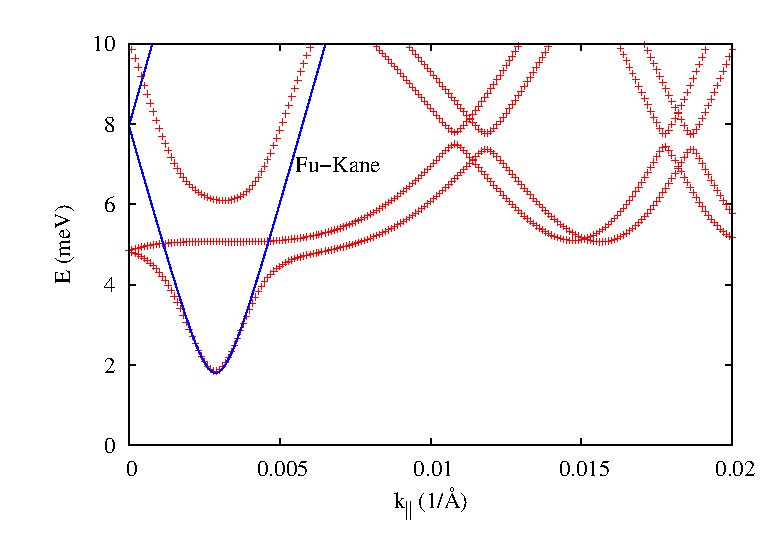
\includegraphics[width=\textwidth]{include/levels.eps}
\caption{The lowest few energy levels $\epsilon_n(k_\parallel)$. 
$\mu=0$, $L=160$nm, and the bulk superconducting gap $\Delta_0\sim$5.2meV.
A well-defined interface mode is clearly visible at sub-gap energies.
Solid lines show a fit to the Fu-Kane model, with $\Delta_s=1.8$meV, 
$v_s=2.7$eV\AA, and $\mu_s=7.5$meV.
}\label{lev-fk}
\end{figure}
%%%%%%%%%%%%%%%%%%%%%%%%%%

We have checked the validity of the Fu-Kane model for a variety of chemical potentials.
Representative examples are plotted in Fig. \ref{lev-chem}. In each case, the sub-gap 
mode can be well accounted by the Fu-Kane 
model with suitable choice of parameters. While $\mu_s$ is always different from $\mu$,
numerically we find it scales linearly with $\mu$. At the same time, 
$\Delta_s$ and $v_s$ show no strong dependence on $\mu$ for this set of parameters.
To make sure that the sub-gap mode is indeed localized near the interface, we plot in 
Fig. \ref{sp} the $z$ dependence of the spectral function $N(k_\parallel,z,\omega)$.
%
The spectral weight of the sub-gap mode is peaked near the interface and decays over 
a length scale $\sim \xi_0$ into the superconductor. This result clearly shows
that for strongly coupled S-TI interfaces, the Fu-Kane model actually describe a
rather ``fat" interface mode. Note that the spectral weight on the TI side 
(not shown in the figure) is finite, 
but it is much smaller in magnitude and decays very fast inside TI. Finally,
Fig. \ref{dos} shows the local density of states near the interface.
The interface mode leads to finite density of states below the bulk gap,
but the spectral weight is very small.

%%%%%%%%%%%%%%%%%%%%%%%%%%
\begin{figure}
\center
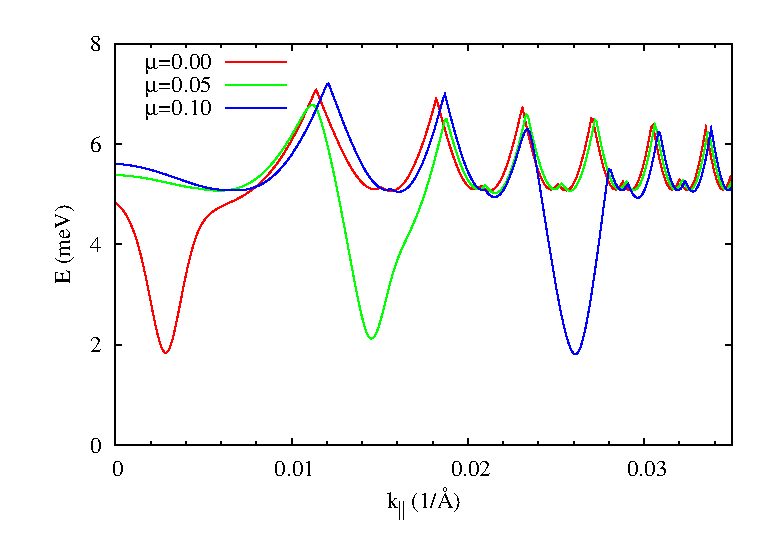
\includegraphics[width=\textwidth]{include/disp-mu.eps}
\caption{The dispersion of the lowest energy level
for different $\mu$ (in eV). Other parameters
are the same as in Fig. \ref{lev-fk}, $L=160$nm and $\Delta_0\sim$5.2meV. Fu-Kane model
well describes the lowest energy mode. As $\mu$ is increased, 
$\Delta_s$ and $v_s$ stay roughly the same, while $\mu_s$ scales
linearly with $\mu$.
}\label{lev-chem}
\end{figure}
%%%%%%%%%%%%%%%%%%%%%%%%%%

%%%%%%%%%%%%%%%%%%%%%%%%%%
\begin{figure}
\center
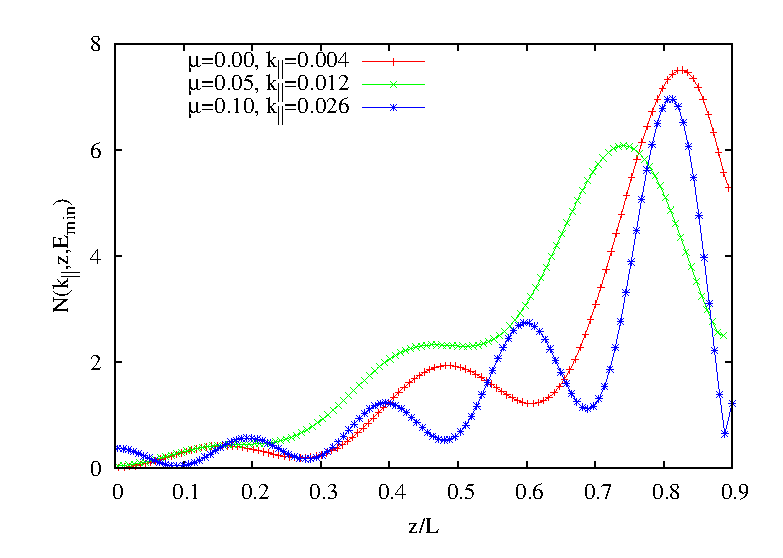
\includegraphics[width=\textwidth]{include/spweight.eps}
\caption{The spectral function $N(k_\parallel,z,\omega)$ of the lowest 
energy level, $\omega=E_{min}$, shown in Fig. \ref{lev-chem}. 
The interface is at $z=0.9L$, $L$=160nm.
The spectral function oscillates rapidly with $z$, so only its envelope is plotted.
}\label{sp}
\end{figure}
%%%%%%%%%%%%%%%%%%%%%%%%%%

We have carried out similar analysis for superconductors with larger
coherence length. Fig. \ref{level-27} shows the evolution of
the sub-gap mode with $\mu$ for $\Delta_0=2.4$meV. In this case,
the values of $(\Delta_s,v_s,\mu_s)$ all varies with $\mu$. 
Superconductors with larger $\xi_0$ and smaller $\Delta_0$ are thus more
sensitive to changes in $\mu$ and other microscopic details near
the interface. The exact values of the effective parameters 
in the Fu-Kane model in general depend on such microscopic details.

%%%%%%%%%%%%%%%%%%%%%%%%%%
\begin{figure}
\center
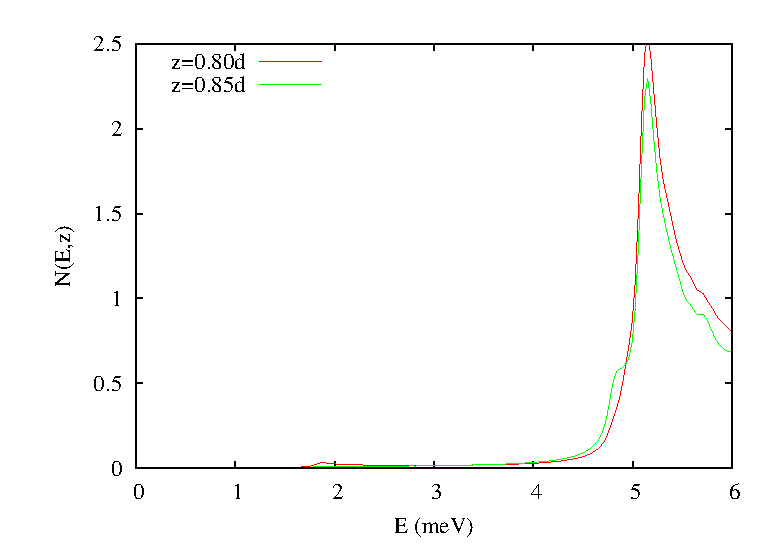
\includegraphics[width=\textwidth]{include/dos.eps}
\caption{The local density of states $N(E,z)$
at $z=0.8d$ and $z=0.85d$ (the interface is at $z=0.9d$).
$\mu=0$, $L=160$nm, and $\Delta_0\sim$5.2meV. The subgap
states are due to the interface mode. A level broadening
$\sim 0.01\Delta_0$ is used.
}\label{dos}
\end{figure}
%%%%%%%%%%%%%%%%%%%%%%%%%%

%%%%%%%%%%%%%%%%%%%%%%%%%%
\begin{figure}
\center
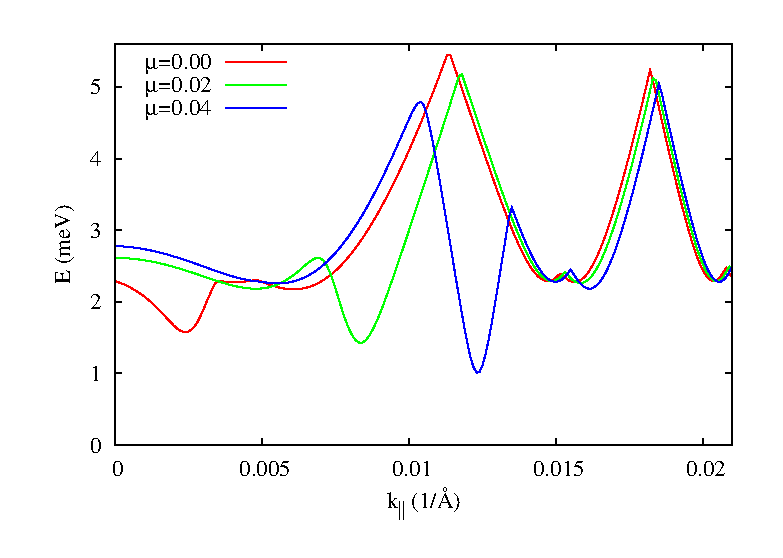
\includegraphics[width=\textwidth]{include/spg27.eps}
\caption{The lowest energy level of an S-TI structure with $L=160$nm,
$d=0.9L$, $\Delta_0=2.4$meV. $\mu$ is the chemical potential of the TI and
measured in eV.}\label{level-27}
\end{figure}
%%%%%%%%%%%%%%%%%%%%%%%%%%

\section{Triplet Pair Correlations}

It is well known that in heterostructures of $s$-wave superconductors,
pairing correlations in other orbital channels, e.g. $p$-wave correlations, 
will be induced by scattering at the interfaces \cite{esch,tanaka}. For example,
inversion/reflection symmetry ($z\leftrightarrow -z$) is lost in an S-TI proximity 
structure, and the appearance of $p$-wave correlations seems natural from
 partial wave analysis. Moreover, scattering by a topological insulator is 
spin-active. The spin-orbit coupling inside a TI acts like a momentum-dependent
magnetic field to flip the electron spin and introduce different phase shifts
for spin up and down electrons. The scattering matrix has been worked out by us 
previously \cite{zhao}. Thus, a singlet $s$-wave Cooper pair can be converted into a pair
of electrons in spin-triplet state at the S-TI interface.
However, it is important to recall that by assumption attractive interaction only exists
(or is appreciable) in the $s$-wave channel. There is no binding force
to sustain a triplet Cooper pair or a triplet superconducting order parameter. 
%
Similar (but different) pairing correlations in superconductor-ferromagnet
hybrid structures have been extensively studied \cite{esch}. 
The appearance of $p$-wave correlations in S-TI systems
has been pointed out previously by Stanescu et al using a perturbative analysis \cite{stan}.

We focus on the equal-time pair correlation functions defined in Eq. \eqref{pair-corr}.
By exploiting the symmetry of the BdG Hamiltonian, Eq. \eqref{symm}, we are able to
find analytically the orbital structure of the triplet correlation functions. The unitary 
transformation Eq. \eqref{unit} yields
\begin{align}
u_{2\uparrow}(k_x,k_y)=u_{2\uparrow}(k_\parallel,0)e^{-i\varphi_k/2},\nn \\
u_{2\downarrow}(k_x,k_y)=u_{2\downarrow}(k_\parallel,0)e^{+i\varphi_k/2},\nn \\
v_{2\uparrow}(k_x,k_y)=v_{2\uparrow}(k_\parallel,0)e^{+i\varphi_k/2},\nn \\
v_{2\downarrow}(k_x,k_y)=v_{2\downarrow}(k_\parallel,0)e^{-i\varphi_k/2}. 
\end{align}
Using these relations, we find
\begin{align}
F_{\uparrow\uparrow}(\kperp,z)=F_{\uparrow\uparrow}(k_\parallel,z)e^{-i\varphi_k},\\
F_{\downarrow\downarrow}(\kperp,z)=F_{\downarrow\downarrow}(k_\parallel,z)e^{+i\varphi_k}.
\end{align}
Namely $F_{\uparrow\uparrow}$ ($F_{\downarrow\downarrow}$) has $p_x-ip_y$ ($p_x+ip_y$) orbital 
symmetry. Finally, the remaining triplet correlation function
\begin{equation}
\langle \psi_{2\uparrow}(\kperp,z) \psi_{2\downarrow} (-\kperp,z)+ \psi_{2\downarrow}(\kperp,z) \psi_{2\uparrow}(-\kperp,z)\rangle
\end{equation}
turns out to be zero. Note that the so-called odd-frequency paring correlations 
\cite{esch,tanaka,trip}, which vanishes in the equal-time limit, 
are also interesting in S-TI structures, but 
we will not discuss their behaviors here.

%%%%%%%%%%%%%%%%%%%%%%%%%%
\begin{figure}
\center
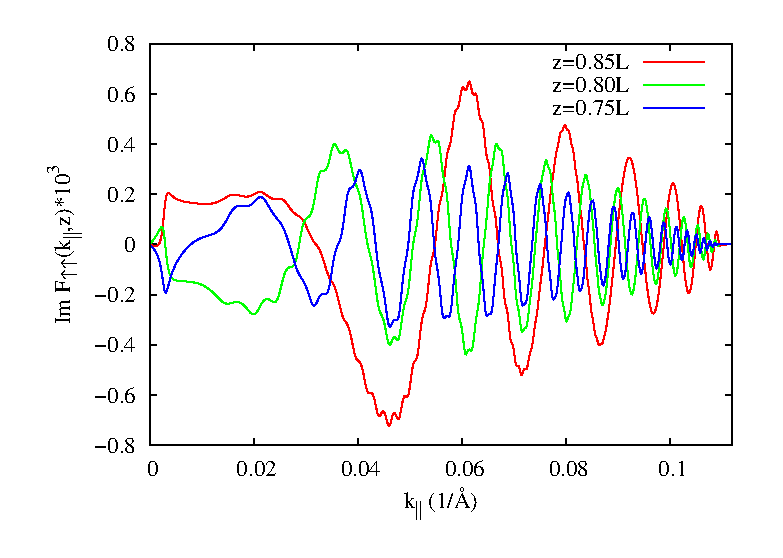
\includegraphics[width=\textwidth]{include/pwave.eps}
\caption{The imaginary part of triplet pair correlation function 
$F_{\uparrow\uparrow}(k_\parallel,z)$. The S-TI interface is at
$d=0.9L$. $\mu=0$, $L=160$nm, $\Delta_0=5.2$meV.
}\label{pw}
\end{figure}
%%%%%%%%%%%%%%%%%%%%%%%%%%

We find that $F_{\uparrow\uparrow}(k_\parallel,z)$ is 
purely imaginary and identical to $F_{\downarrow\downarrow}(k_\parallel,z)$.
The results for $\mu=0$, $L=160$nm, $d=0.9L$, $\Delta_0=5.2$meV are plotted
in Fig. \ref{pw}. $F_{\uparrow\uparrow}$ vanishes at $k_\parallel=0$
as well as for large $k_\parallel$, namely when $k_\parallel>\sqrt{(E_F+\omega_D+M)/B_2}$.
This is consistent with lack of pairing in both limits. 
The behavior of $F_{\uparrow\uparrow}$ for small $k_\parallel$
is illustrated in Fig. \ref{pw-cu} for $\mu=0$, $L=300$nm, $d=0.95L$, 
$\Delta_0=0.6$meV. As comparison, we also plotted the singlet
 pair correlation function 
\begin{equation}
F_{\uparrow\downarrow}(\mathbf{k}_\parallel,z)=\sum'_n u_{n,2\uparrow}(\mathbf{k}_\parallel,z)
v^*_{n,2\downarrow}(-\mathbf{k}_\parallel,z)
\end{equation}
which is $s$-wave and purely real.

%%%%%%%%%%%%%%%%%%%%%%%%%%
\begin{figure}
\center
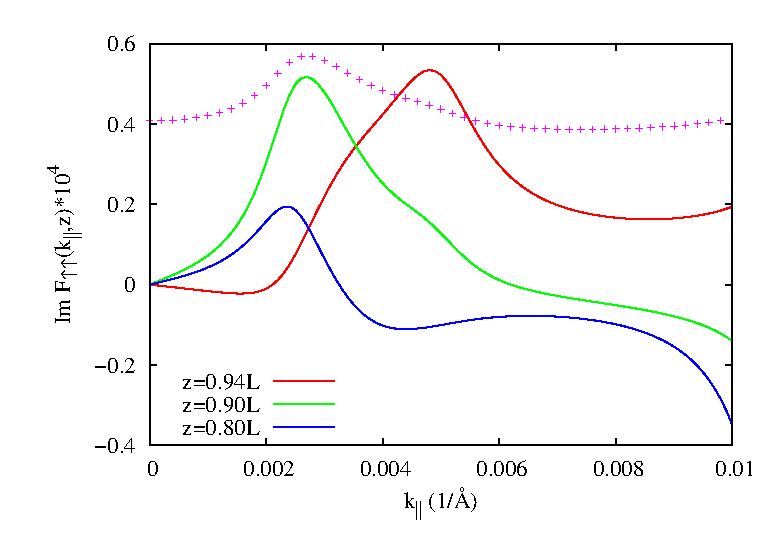
\includegraphics[width=\textwidth]{include/pw-cu.eps}
\caption{The imaginary part of 
$F_{\uparrow\uparrow}(k_\parallel,z)$. $\mu=0$, $L=300$nm, $d=0.95L$, $\Delta_0=0.6$meV.
As comparison, the data points show the singlet pair correlation function 
$F_{\uparrow\downarrow}(k_\parallel,z=0.9L)/3$.
}\label{pw-cu}
\end{figure}
%%%%%%%%%%%%%%%%%%%%%%%%%%

\section{Summary}
In summary, we have investigated the proximity effect between an $s$-wave superconductor
and a topological insulator using a microscopic continuum model. 
Strong coupling between the two materials renders the surface state of TI a less 
useful concept for this problem.
Our focus has been on the various modifications to superconductivity by the presence of TI. 
These include the suppression of the order parameter, the formation of interface modes
below the bulk superconducting gap, and the induction of triplet pairing correlations.
It is gratifying to see the Fu-Kane effective model emerges in the low energy sector
albeit with a set of renormalized parameters. Our results are complementary to
previous theoretical work on the proximity effect \cite{f-k,stan} and confirm the validity
of the Fu-Kane model.

We made a few simplifying assumptions in our calculation. The superconductor is described 
by a two-band model with the valence band well below the Fermi level. Since only 
electrons near the Fermi surface are relevant for weak coupling superconductivity, we 
believe our main results are general. As idealizations, the chemical 
potential, the spin-orbit coupling, and the attractive interaction are assumed to be 
step functions with a sudden jump at the interface. 
More elaborate and realistic models can be considered within the framework of BdG equations.
For example, one can add a tunneling barrier between S and TI, 
or include a Rashba-type spin-orbit coupling term 
(due to the gradient of chemical potential) at the interface. We will not 
pursuit these generalizations here.
Finally, the approach outlined here can be straightforwardly applied to 
study non-Abelian superconductivity in other superconductor-semiconductor
heterostructures where spin-orbit coupling also plays a significant role
\cite{roman,maryland,jason,mao1,mao2}.




\chapter{Josephson Junction on TI Surface}

So far, we have found that the regions near the interface, between the topological insulator and a superconductor, is an exotic playground to interesting phenomena, namely a subgap energy state localized near the interface. This two dimensional interface considered to be the Fu-Kane superconductor and modeled by a Dirac-like relativistic equation
\begin{equation}
\mathcal{H}=-i\hbar v_F(\sigma_x  \partial_y - \tau_z\sigma_y \partial_x) + \tau_z \mu + \tau_y \sigma_y \Delta
\end{equation}
is good up to some renormalization of the constants, $v_F$, $\mu$, $\Delta$ as found in the previous chapter. This model was used in the first chapter to illustrate the existence of Majorana bound states localized where the effective mass term, $\Delta$, changes sign ($\Delta\rightarrow -\Delta$) as in a Josephson $\pi$ junction. This Majorana mode has a linear dispersion, $E\propto \pm k$.
In this chapter we explore this $\pi$ junction further, in particular for $\mu \neq 0$, where we find an energy dispersion that is flat and follows as $E \propto k^{N}$, where $N$ scales with $\mu$.
An extension of the the $\pi$ junction is a periodic $\pi$ junction where alternating ($...-\Delta,\Delta,-\Delta,\Delta...$) stripes of superconductors are placed in one direction. We find that this system also hosts the flat dispersion. We also find that the dispersion has ``wiggles'' when the spectrum is really closely analyzed. 

\section{Introduction}

Moving at ``the speed of light", $v_F$,
massless Dirac electrons on the surface of a three-dimensional $Z_2$ topological insulator (TI) can not be localized by scattering from nonmagnetic impurities \cite{hasan_colloquium:_2010,qi_topological_2011}, nor can they be
easily confined by electrostatic potentials due to Klein tunneling \cite{Katsnelson:2006fk}. Proximity coupling to 
ferromagnetic or superconducting order can however 
open up a gap in the spectrum, thus rendering excitations massive \cite{hasan_colloquium:_2010,qi_topological_2011}.
 An intriguing
possibility is to engineer new {\it massless} excitations by confining and coherently mixing Dirac electrons 
and holes using two or more superconductors with definite phase difference \cite{fu_superconducting_2008}.
For example, Fu and Kane showed that a Josephson junction on the surface of a TI with a phase bias of $\pi$ is a one-dimensional quantum wire for Majorana fermions, 
which can be further manipulated by using tri-junctions \cite{fu_superconducting_2008}. Signatures of Majorana fermions in such structures have been reported in recent 
experiments \cite{williams_unconventional_2012,moore_extraordinary_2012}.

In this Letter, we demonstrate a drastically different regime for the same, albeit slightly more general, Josephson structures considered by Fu and Kane.
This regime features massless zero energy excitations that are almost dispersion-less, i.e. with vanishing group velocity $(\partial E/\partial k\simeq0)$.
We elucidate the scattering kinematics behind the nearly flat dispersion at zero energy using simple models, and verify the results with self-consistent calculations.
We find it striking that in such simple structures, which are now available in experiments, the low energy excitation can be easily tuned all the way from $E\sim k$ to $E\sim k^N$, where $N$ is large, by increasing the chemical potential. 
%We further show that \red{the extension of such junctions into} a class of {\it periodic} \red{superconductor-TI proximity structures also become} flat at zero energy.
By extending such junctions into a class of {\it periodic} superconductor-TI proximity structures, we further show that these states become a flat band near zero energy.

\section{Model}
The Josephson junction is schematically shown in Fig.~\ref{jjsetup}a). Two $s$-wave superconductors are patterned
on the TI surface. Due to the proximity effect, the S-TI interface becomes a 2D superconductor (S).
The S-TI-S junction can be well described by the following Bogoliubov-Dirac Hamiltonian introduced in Ref. \cite{fu_superconducting_2008},
\begin{equation}
\mathcal{H}=\hbar v_F(\sigma_x k_y +i \tau_z\sigma_y \partial_x) + \tau_z \mu(x) + \tau_y \sigma_y \Delta(x).
\label{ham}
\end{equation}
Here $\tau_i$ ($\sigma_i$) are the Pauli matrices in the particle-hole (spin) space. 
The system is translationally invariant in the $y$ direction, and $k_y$ is the momentum along $y$. 
In the TI region of 
length $w$, the superconducting order parameter $\Delta(x)$=0, while it is constant $\Delta$ deep into the superconductor. 
The chemical potential $\mu$ can be tuned by applying a gate voltage.
In general, its value can differ in the TI and S region, but for simplicity,
we assume it is uniform in all regions. 
Also, we will focus on the case of phase difference of $\pi$ across the junction.

 %%%%%%%%%%%%%%%%%%%%%%%%%%
\begin{figure}
\center
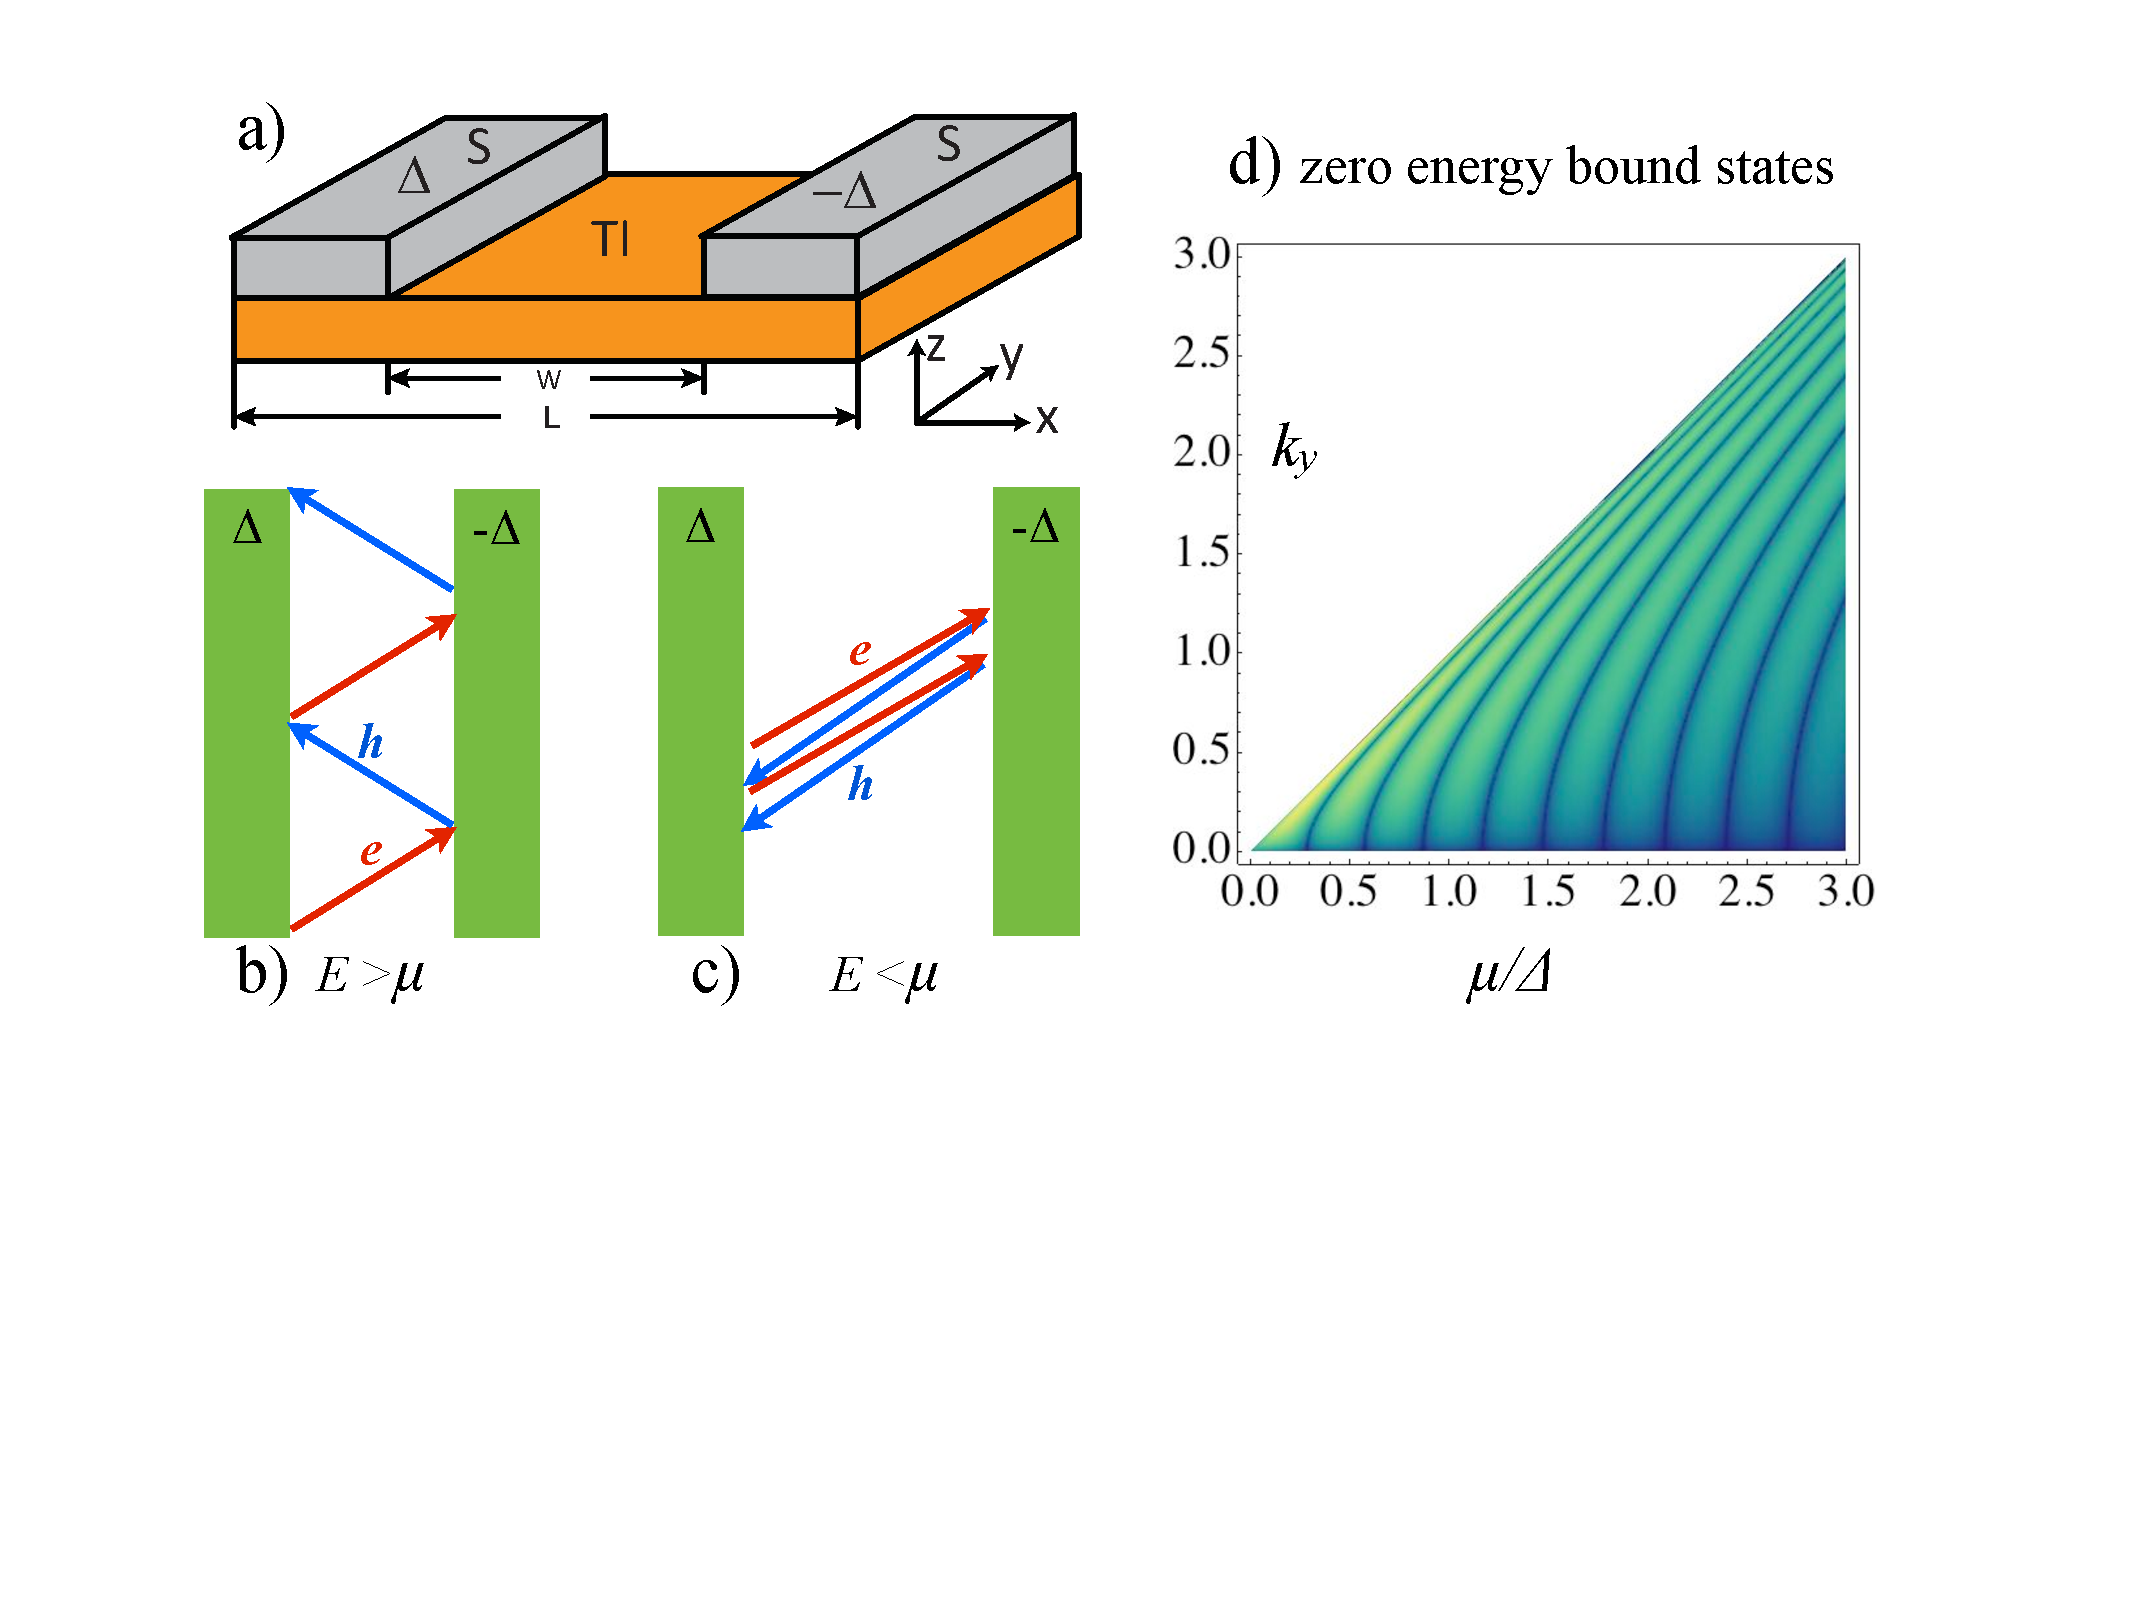
\includegraphics[width=\textwidth]{include/fig1.pdf}
\caption{(color online) a) Schematic of a Josephson junction on the surface of a topological insulator (TI).
The two superconducting leads (S) have a phase difference $\pi$. $\Delta$ is the superconducting gap, and 
$w$ is the junction width (not to scale).
b) Specular Andreev reflection in the regime $E>\mu$. c) Retro-reflection for $E<\mu$.
d) Dark lines show the $(k_y,\mu)$ values for the zero energy Andreev bound states for $w=10\hbar v_F/\Delta$ 
and $L\rightarrow \infty$.
$k_y$ is in unit of $\Delta/\hbar v_F$.
}\label{jjsetup}
\end{figure}
%%%%%%%%%%%%%%%%%%%%%%%%%%

We first give a heuristic argument for the existence of two regimes.
A Dirac electron in the TI region incident on S will be Andreev reflected into a hole if its energy is below the superconducting gap ($E<\Delta$). 
In the context of graphene \cite{PhysRevLett.97.067007,RevModPhys.80.1337}, 
Beenakker pointed out that in addition to the familiar Andreev retro-reflection where the reflected hole has a group velocity opposite to the incident electron when $E<\mu$, 
there is also the case of specular Andreev reflection where the reflected hole's group velocity is in the specular direction for $E>\mu$. Typical scattering trajectories in these two regimes are contrasted in Fig.~\ref{jjsetup}b) and \ref{jjsetup}c).
For $\mu=0$ as considered in Ref.~ \cite{fu_superconducting_2008}, 
the Majorana fermion excitation with linear dispersion is associated with the specular Andreev reflections in Fig.~\ref{jjsetup}b). 
For large $\mu$, as in the case of as grown Bi$_2$Se$_3$ crystals, one expects very different behaviors at low energies. 
For the $E<\mu$ case, it can be shown analytically that the phase of the retro-reflected hole is equal to the incident angle of an incoming electron at zero energy, $\theta=\arcsin(\hbar v_F k_y/\mu)$. This is unique to TIs because the wavefunction of a Dirac electron [or hole], $(1,\pm e^{i\theta},0,0)$ $[(0,0,1,\pm e^{i\theta})]$, 
is determined by the angle $\theta$, or $k_y$. The resultant hole incident on the opposite S with phase of $\pi$ retro-reflects into an electron. This electron has exactly the same phase as it started with, thus forming an Andreev bound state. 


The remaining key question is whether there will be any states at or near 
zero energy when $\mu$ is finite. We can answer the question by solving 
Eq.~(\ref{ham}) for an idealized, step function profile of $\Delta(x)$,
\begin{equation}
\Delta(x) = \Delta[\theta(-x)-\theta(x-w)].
\end{equation}
The dark lines in Fig.~\ref{jjsetup}d) shows the zero energy solution in the 
$(\mu,k_y)$ plane, with fixed $\Delta$ and the junction length $w=10\hbar v_F/\Delta$. 
In general, there exist multiple zero energy bound states
at discrete $k_y$ values $\{k_y^i\}$ for finite $\mu$. 
For increasing $\mu$ and  $w$,
these solutions become increasingly close-packed.
This nontrivial result has important implications for experiments. 
The Majorana quantum wire is only ideal in the limit of $\mu,w\rightarrow 0$.
As $\mu$ is tuned away from the Dirac point, the single zero energy state at $k=0$ will 
be replaced by multiple zero energy solutions
along the $k_y$ axis, and eventually a nearly flat dispersion at zero energy.

To unambiguously establish this claim, we solve the differential
equation $\mathcal{H}(x,k_y)\psi(x,k_y)=E \psi(x,k_y)$ numerically 
for a finite size system, $x\in [0,L]$ as shown in Fig.~\ref{jjsetup}a),
with open boundary conditions at $x=0,L$ \cite{footnote1}. Here the quasiparticle wave function
$\psi=\left ( { u} _{\uparrow},  { u}_{\downarrow},  { v}_{\uparrow}, { v}_{\downarrow} \right )^T$,
with the label $(x,k_y)$ omitted.
To fully describe the proximity
effect including the induced superconducting correlations in the TI region
and the suppression of superconductivity near the TI-S boundary, we 
determine the order parameter profile $\Delta(x)$ self-consistently
through the gap equation
\begin{equation}
\Delta(x)= g(x)\sum_{\epsilon_n<\omega_D}\int d k_y u_{n,\uparrow}(x,k_y) v_{n,\downarrow}^\ast(x,k_y).
\end{equation}
Here $n$ labels the eigenstates with energy $\epsilon_n$, $g$ is the effective
attractive interaction, and $\omega_D$ is the Debye frequency. We assume $g$
is zero in the TI region and constant inside S. We expand $\psi(x,k_y)$ and 
$\Delta(x)$ in Fourier series and convert the differential equation into 
an algebraic equation~\cite{halterman_characteristic_2011,PhysRevB.83.184511}. Starting with
an initial guess of $\Delta(x)$ which features phase difference 
$\pi$, the iterative procedure is repeated until desired convergence is achieved.
Note that the phase difference $\pi$ is self-maintained throughout and not fixed by hand after every iteration.
Then, the local spectral function,
\begin{equation}
A_\sigma(E,k_y,x)=\sum_n \delta(E-\epsilon_n)|u_{n\sigma}(x,k_y)|^2,
\end{equation} 
and the local density of states (LDOS),
\begin{equation}
N(E,x)=\int dk_y\sum_{n,\sigma} \delta(E-\epsilon_n)|u_{n\sigma}(x,k_y)|^2,
\end{equation} 
can be computed for $\sigma=\uparrow,\downarrow$. The calculation is checked to
reproduce known results, e.g., the linearly dispersing Majorana spectrum
at $\mu=0$ predicted in Ref. \cite{fu_superconducting_2008}.

%%%%%%%%%%%%%%%%%%%
\begin{figure}[]
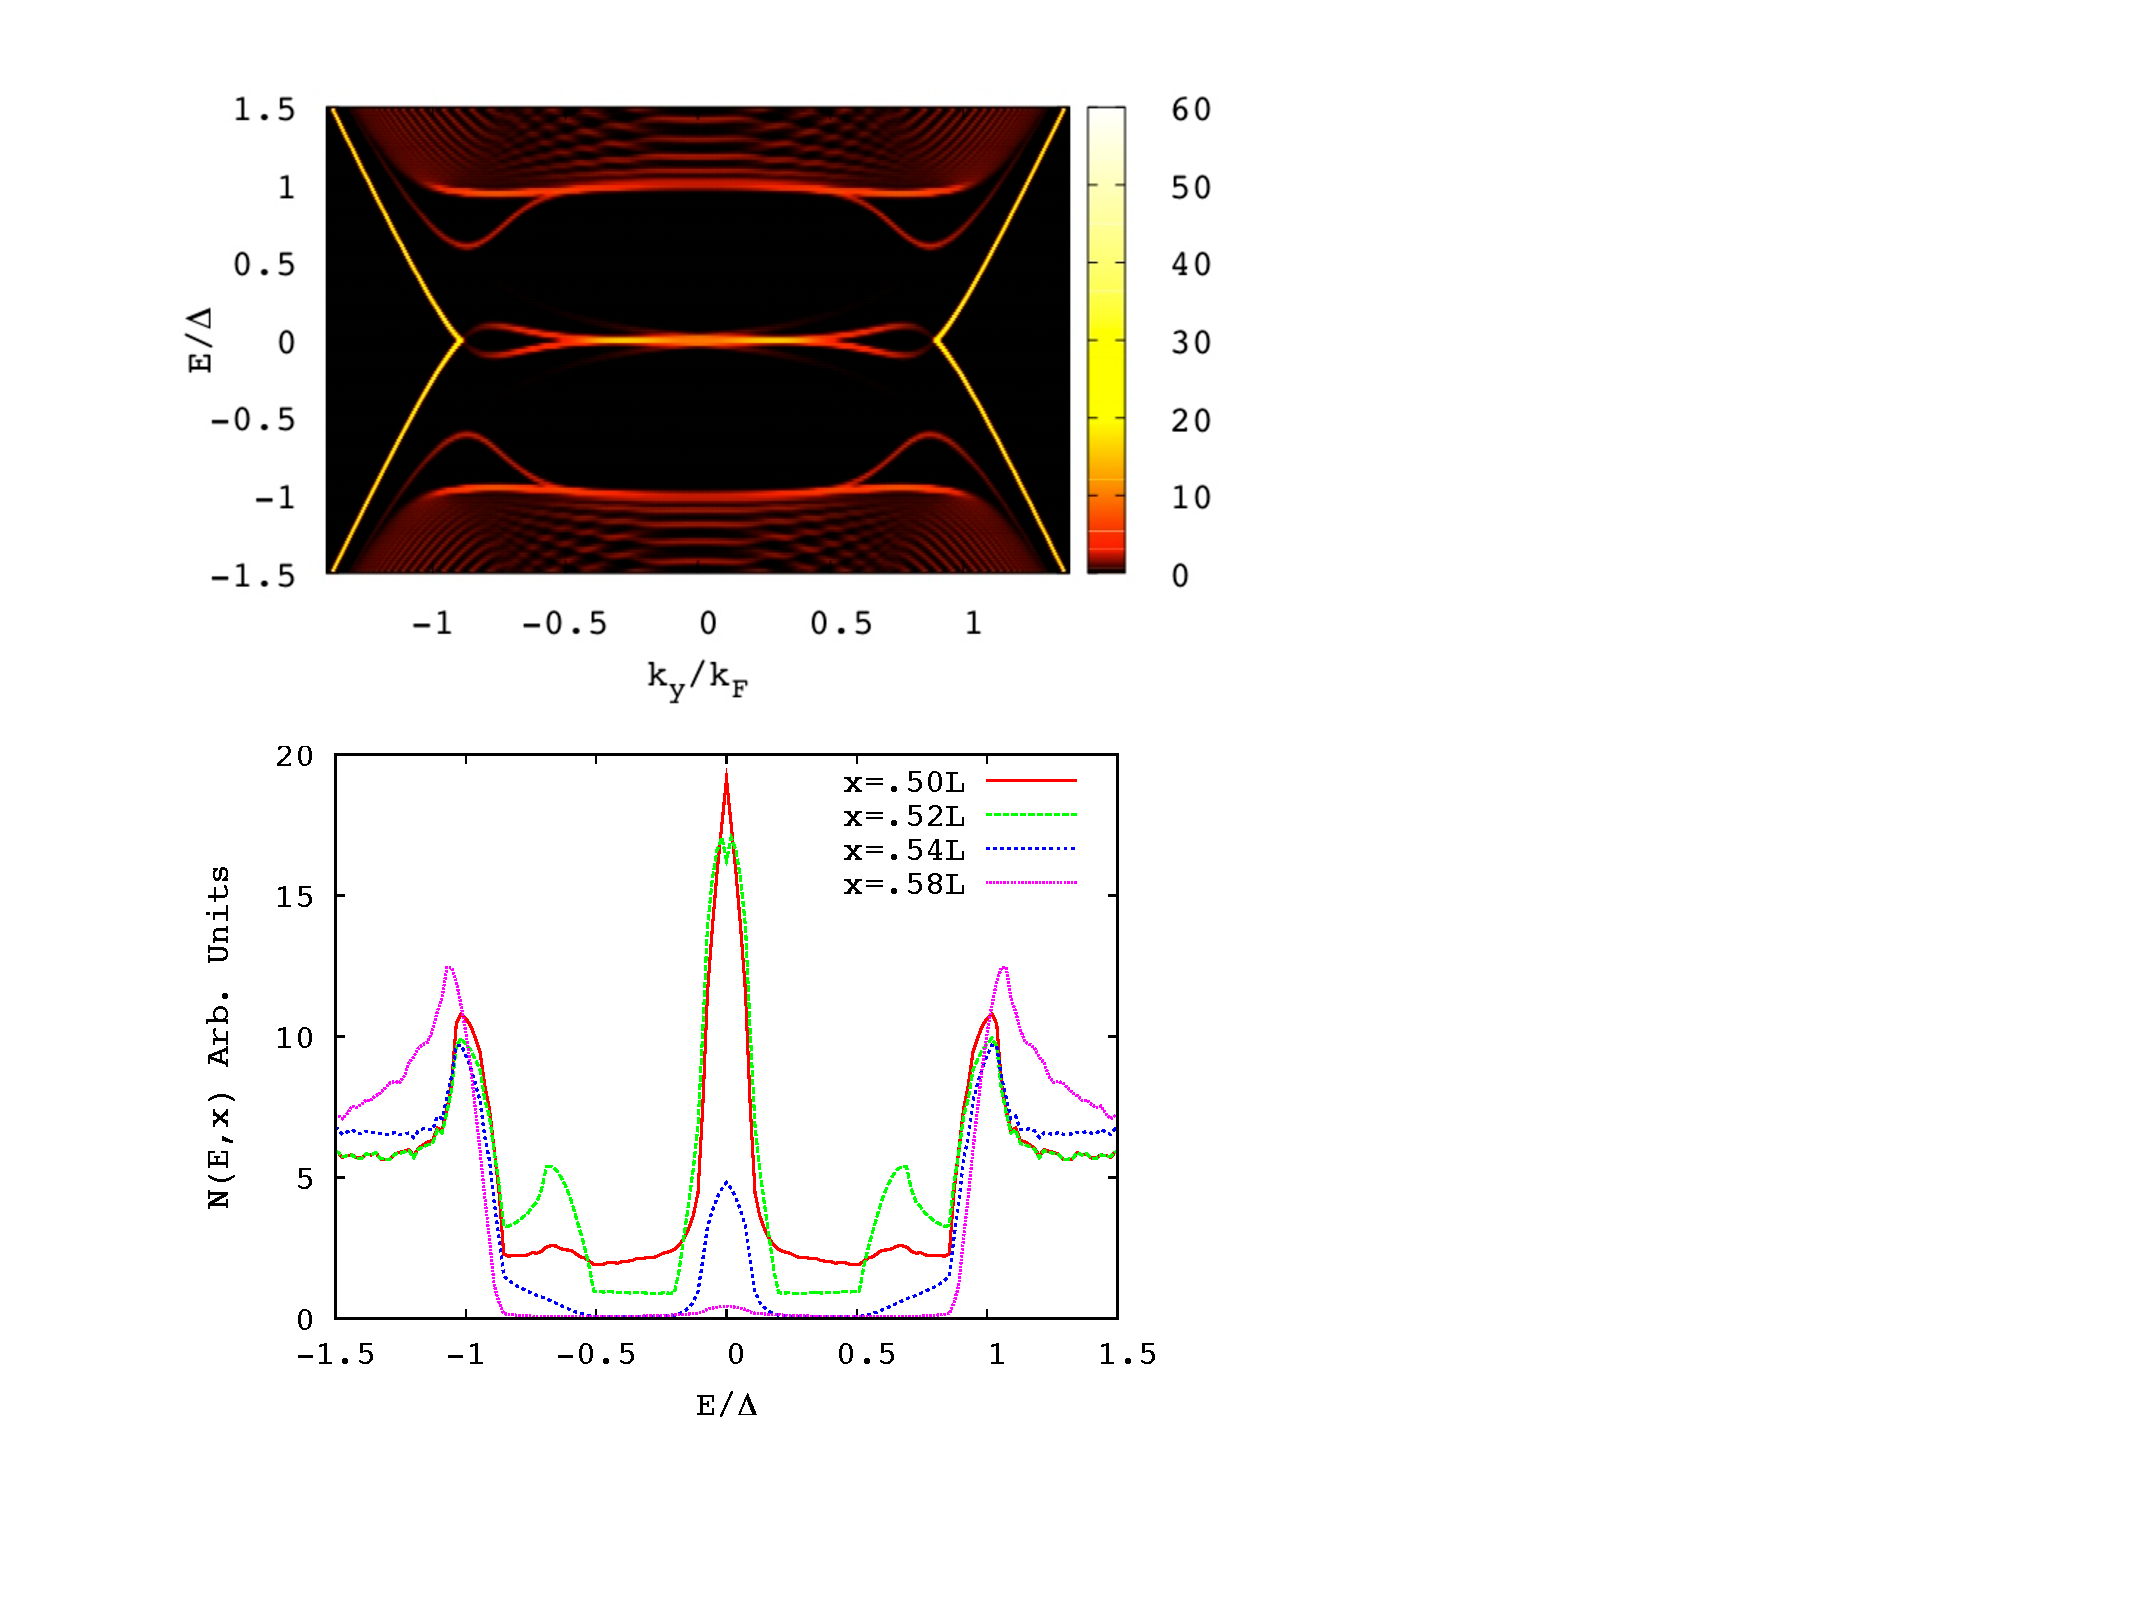
\includegraphics[width=\textwidth]{include/fig2.pdf}
\caption{(color online) The local spectral function $A_\uparrow(E,k_y,x)$
(upper panel) and local density of states $N(E,x)$ (lower panel,
red solid line) at the center of the junction,
$x=0.5L$. One sees ``flat" Andreev bound states near
zero energy for $-k_F<k_y<k_F$, and correspondingly a pronounced peak
at zero energy in the LDOS in the lower panel.
The lower panel also shows different LDOS away from the center,
for $x$ from $0.52L$ to $0.58L$. } \label{dosf}
\end{figure}
%%%%%%%%%%%%%%%%%%%%%

\section{Flat Bands in Spectrum}
The upper panel of Fig. \ref{dosf} shows the spectral function
at the center of the junction, $A_\uparrow(E,k_y,x=0.5L)$ ($A_\downarrow$ is the
same for this value of $x$), with $\mu$=20meV,
$\Delta=5.5$meV,  $w=0.04L$, $L= 2576$nm, 
$ \hbar v_F$=4.1 \AA eV, and the Fermi momentum $k_{F}=\mu/(\hbar v_F)$.
In contrast to the $E\sim \hbar v_F k_y$ mode for $\mu=0$, we see 
Andreev bound states (ABS) near zero energy within a wide region $-k_F<k_y<k_F$,
where the slope $\hbar v_y=\partial E / \partial k_y$ approaches zero. 
The appearance of numerous crossings at exact zero energy for finite $k_y$ 
also agrees with the model calculation above in Fig.~\ref{jjsetup}d). 
%
Beyond this range, e.g. for $k_y>k_F$, the spectrum is reminiscent 
of the particle-hole folded dispersion of the helical metal, 
$E\sim \pm \hbar v_F(k_y- k_F)$.
%

As an approximate ansatz to describe the almost flat dispersion, we introduce the 
following phenomenological model for the ABS for large $\mu\gg \Delta$, 
\begin{equation}
E/\Delta = c (k/k_F)^N,
\label{bigN}
\end{equation}
where $c$ is a constant and $N$ is a large number. To fix $N$, we demand that
the slope of the dispersion at energy $E\sim \Delta$ coincides with that of the bare
dispersion, i.e., $\partial E/\partial k_y|_{E=\Delta}=\hbar v_F$. This gives an estimate
of $N$,
\begin{equation}
N\simeq \mu/\Delta.
\end{equation}
Note that we are only concerned with the ABS dispersion near zero energy and its continuation beyond $k_F$. 
For wider junctions, additional subgap ABS appear at finite energies,
and they are not described by Eq. (\ref{bigN}). Our ansatz is inspired by the 
mathematical theory of Dirac points with multiple topological charge $N$ as found in multi-layered
system discussed in Ref. \cite{flat-N}.

The flat dispersion implies a peak at zero energy in the local density of states. The lower panel of 
Fig. \ref{dosf} shows the LDOS at the center of the junction, at the S-TI boundary, and slightly into
the superconductor for the same junction parameters given above. 
While the zero energy peak becomes less pronounced when away from the junction center, 
it remains clearly visible and persists even into the superconductor. Thus, the predicted flat ABS has a clear
experimental signature in the tunneling conductance measurements.


The existence of two regimes including the flat Andreev bound states near zero energy is a general
feature. We have carried out systematic, self-consistent simulations for the 
general case of an inhomogeneous chemical potential, e.g., $\mu(x)=\mu_{TI}$ 
within the TI region and $\mu(x)=\mu_S\neq \mu_{TI}$ inside the superconductors.
The movie in the Supplementary Material shows the evolution of a typical spectrum for fixed 
$\mu_S$ with $\mu_{TI}$ gradually being increased from zero to $\mu_S$ \cite{footnote2}.
We see the linear Majorana mode changing into the flat ABS.
Select frames from a similar movie are layed out in figures \ref{movie} and \ref{moviedos}. These frames show the evolution from Majorana to flat band as the chemical potential goest from $\mu=0$eV to $\mu=.014$eV in the spectral function, $A(x=.5L,k_y,E)$ and DOS, $N(x=.5L,E)$.

\begin{figure}[h]
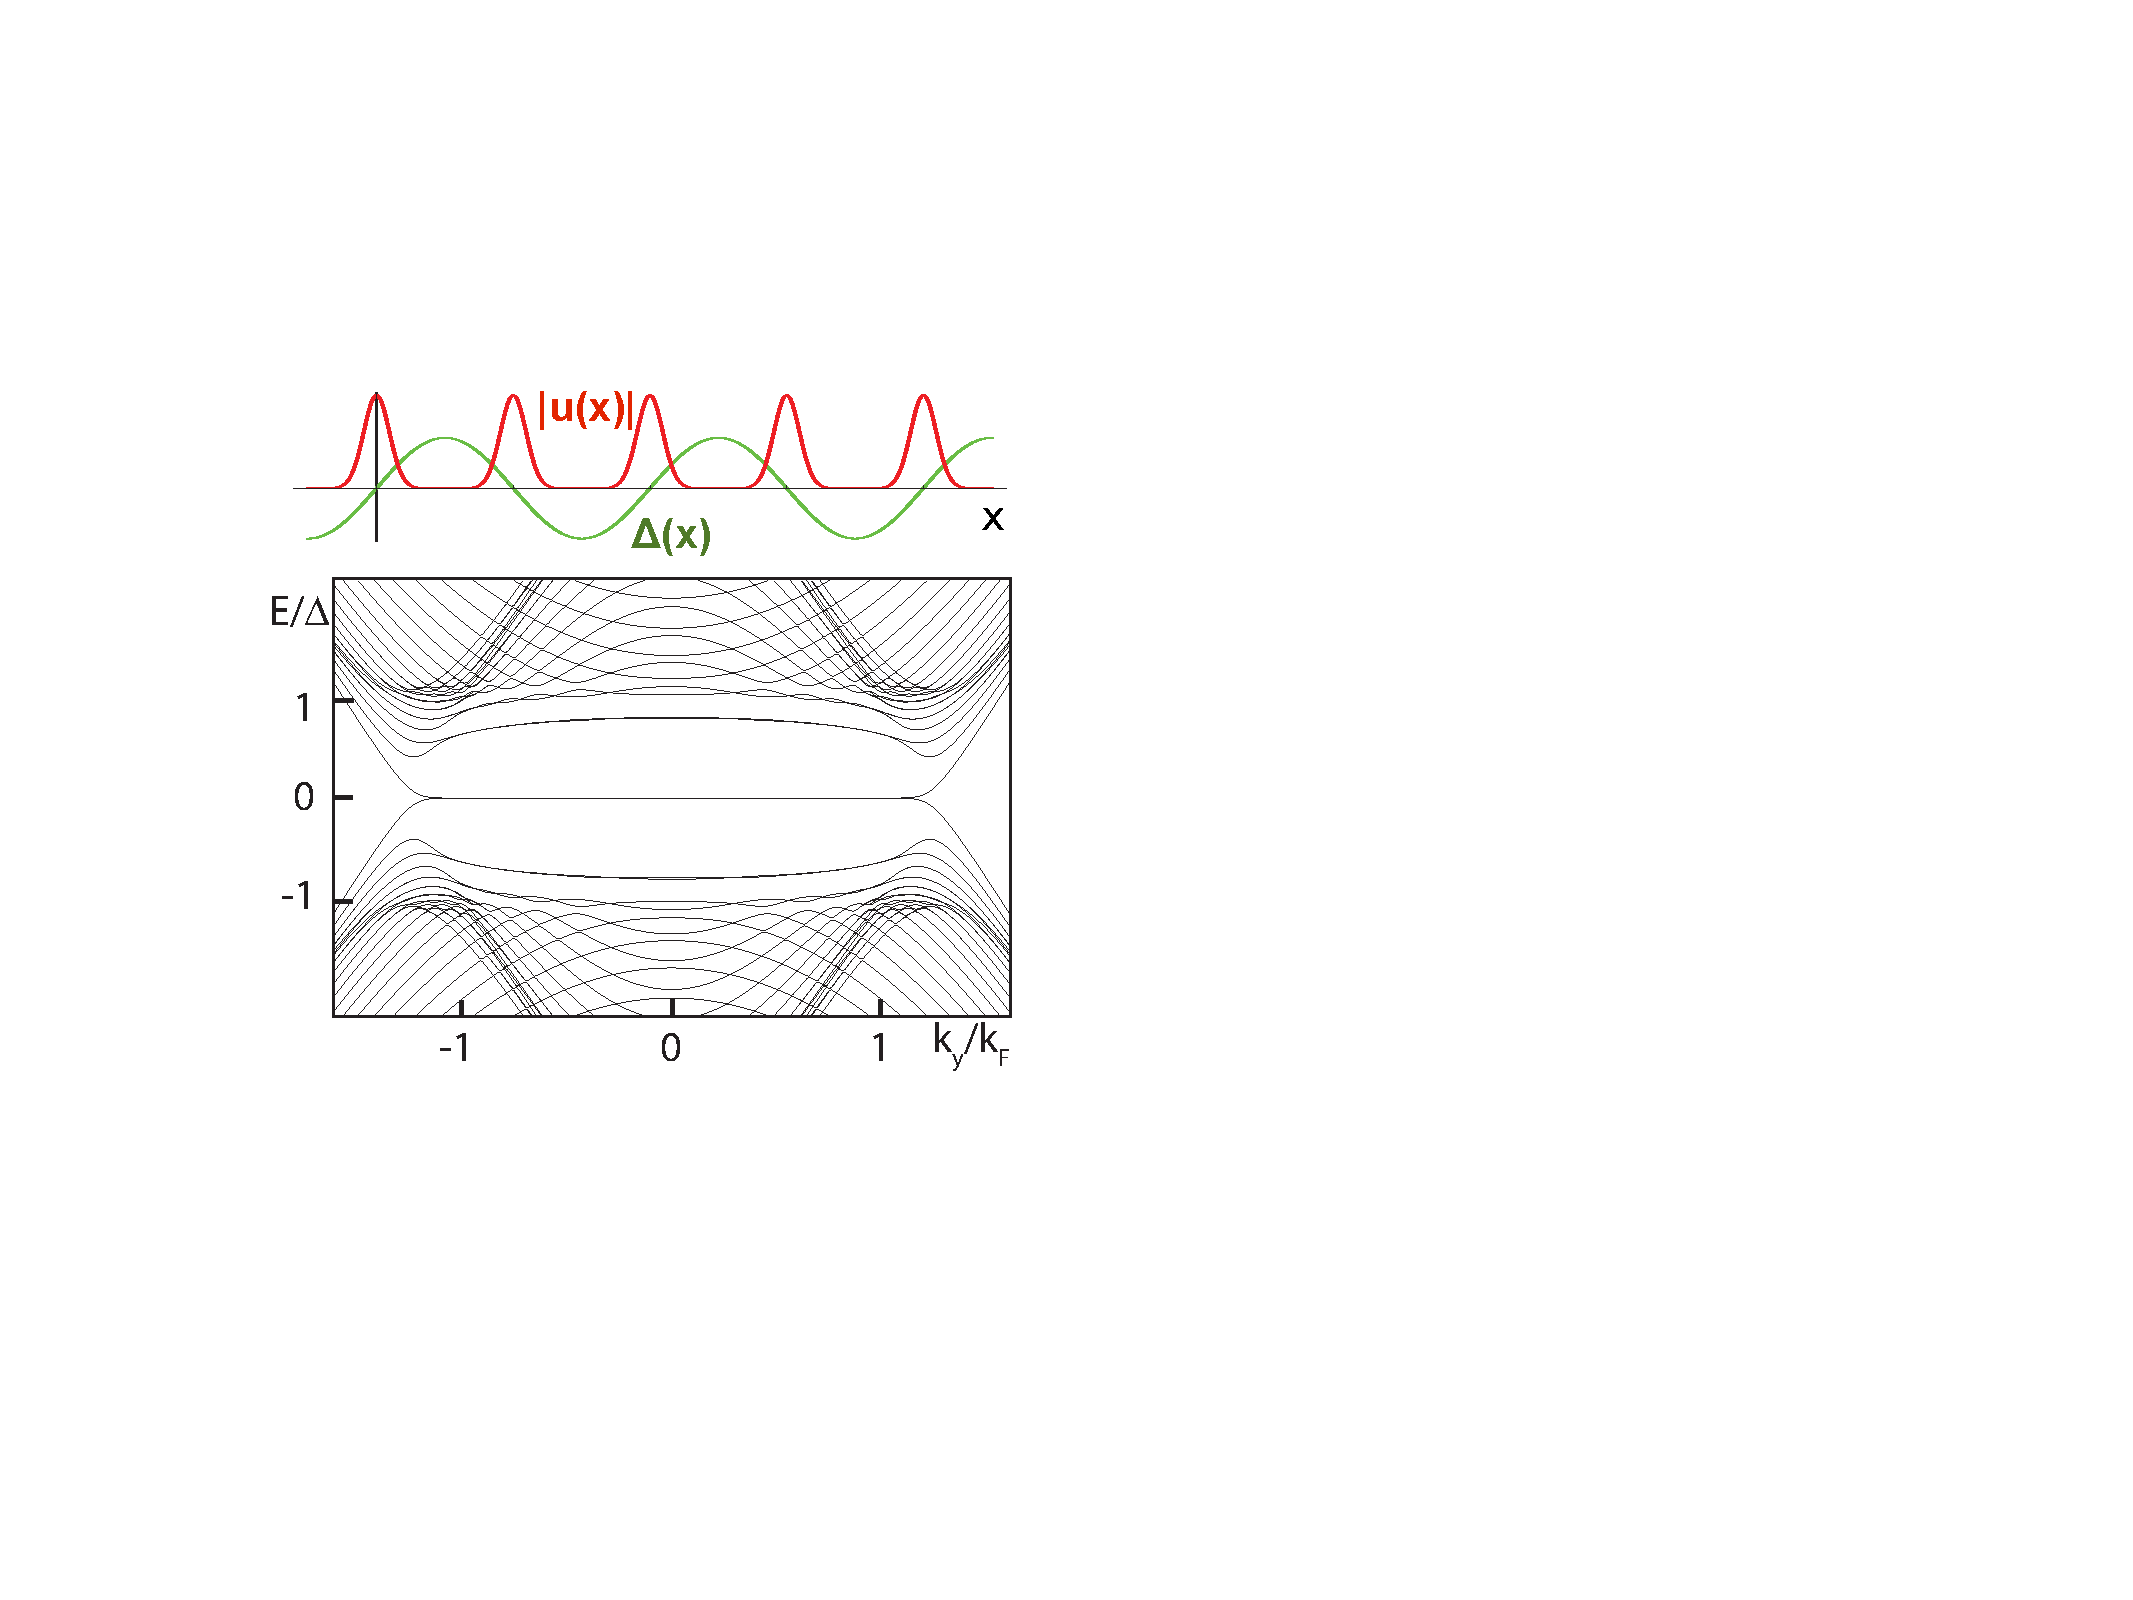
\includegraphics[width=\textwidth]{include/fig3.pdf}
\caption{(color online) Upper panel: Schematic of the periodic proximity structure with 
$\Delta(x)=\Delta  \sin(\pi x/a)$. The wave function $|u(x)|$ for the zero energy states
are peaked at the domain wall boundaries, $x=ma$. Lower panel: Energy spectrum for 
$a=24\hbar v_F/\Delta$ and $\mu=4\Delta$ is flat at zero energy, which has fine structures upon closer inspection.
}\label{array}
\end{figure}


\begin{figure}[h]
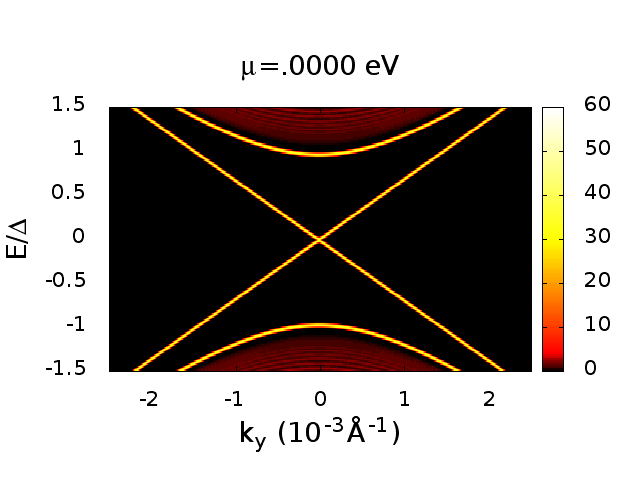
\includegraphics[width=.3\textwidth]{include/spectral/0000.png}
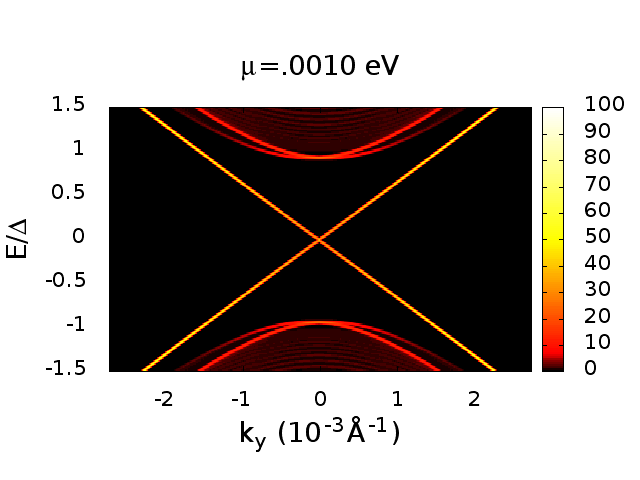
\includegraphics[width=.3\textwidth]{include/spectral/0010.png}
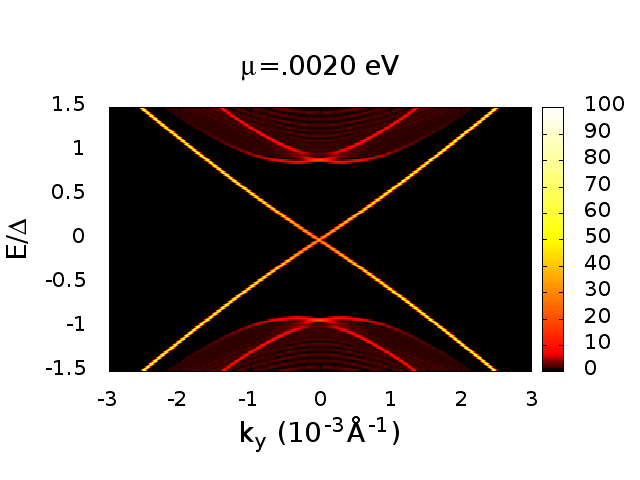
\includegraphics[width=.3\textwidth]{include/spectral/0020.png}\\
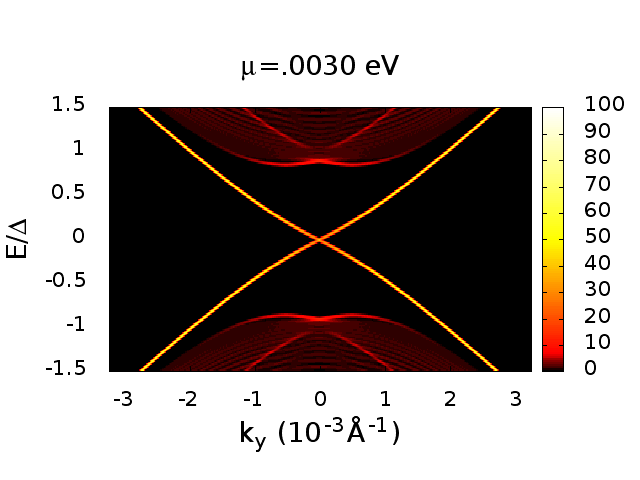
\includegraphics[width=.3\textwidth]{include/spectral/0030.png}
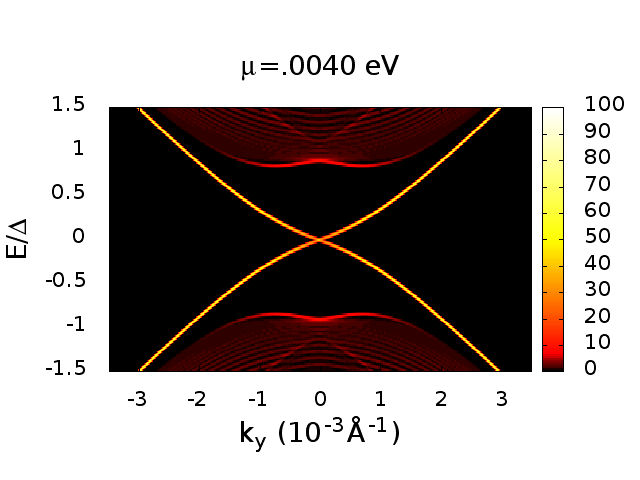
\includegraphics[width=.3\textwidth]{include/spectral/0040.png}
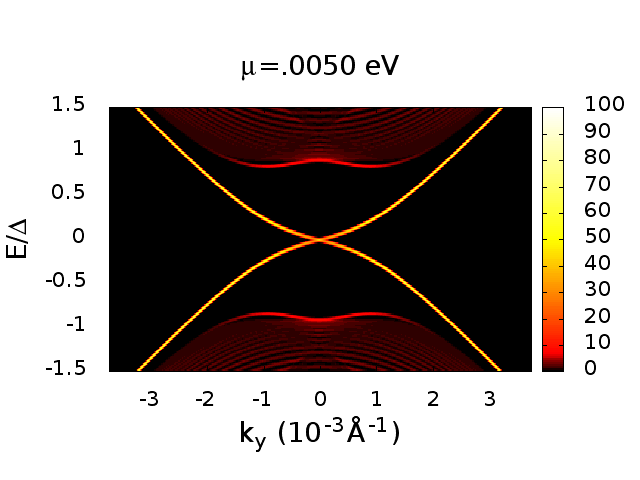
\includegraphics[width=.3\textwidth]{include/spectral/0050.png}\\
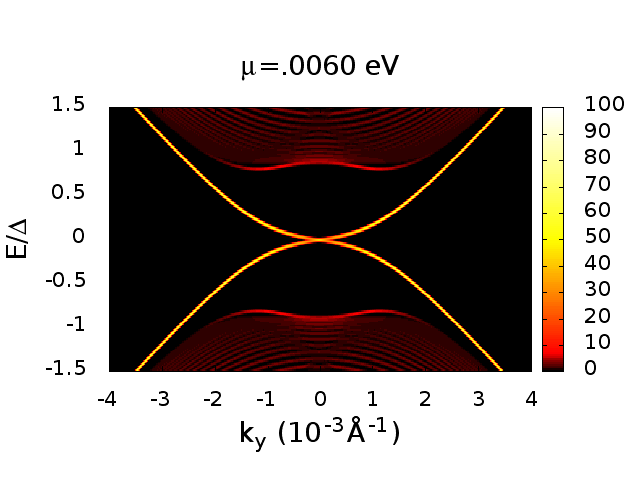
\includegraphics[width=.3\textwidth]{include/spectral/0060.png}
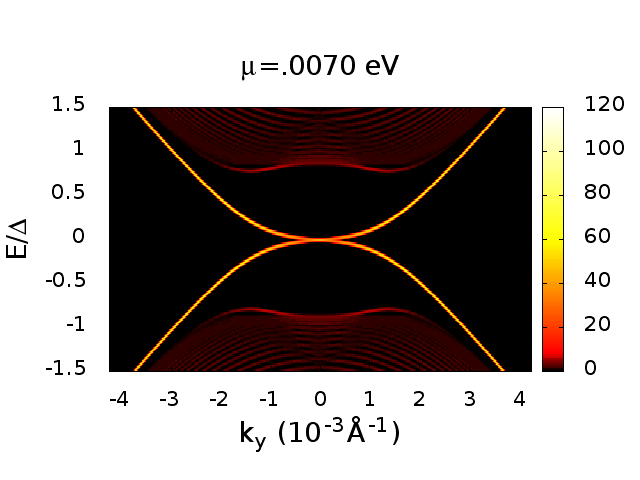
\includegraphics[width=.3\textwidth]{include/spectral/0070.png}
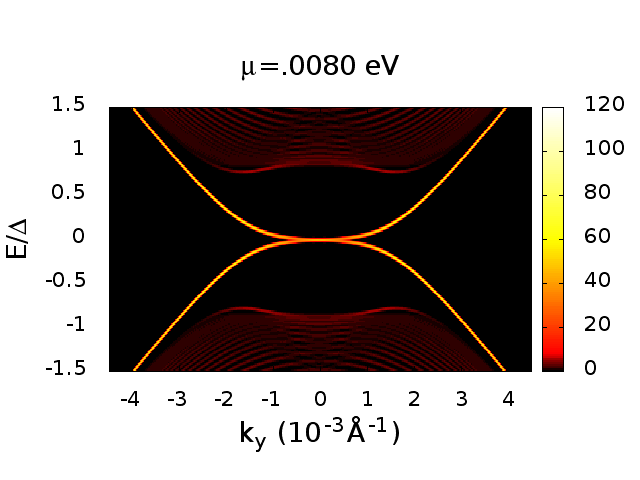
\includegraphics[width=.3\textwidth]{include/spectral/0080.png}\\
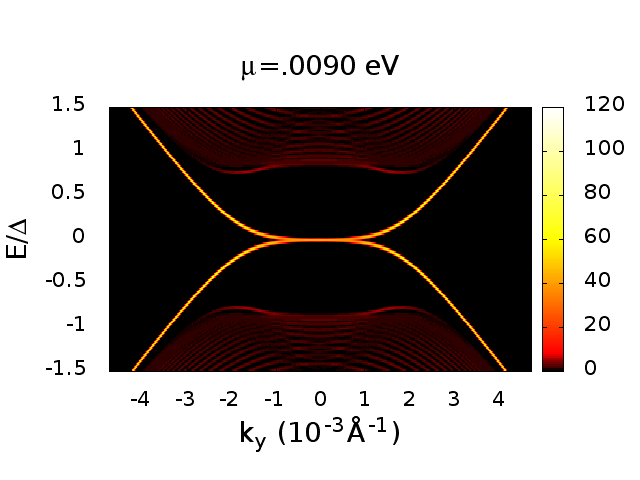
\includegraphics[width=.3\textwidth]{include/spectral/0090.png}
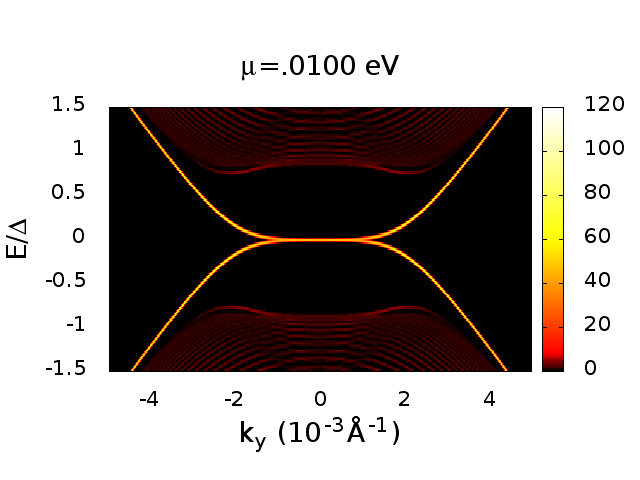
\includegraphics[width=.3\textwidth]{include/spectral/0100.png}
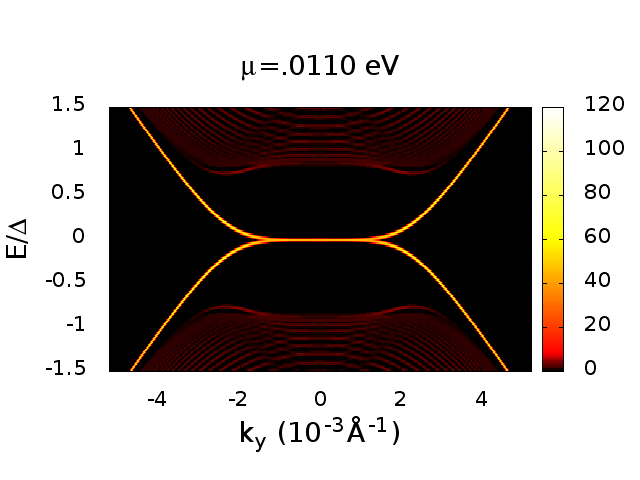
\includegraphics[width=.3\textwidth]{include/spectral/0110.png}\\
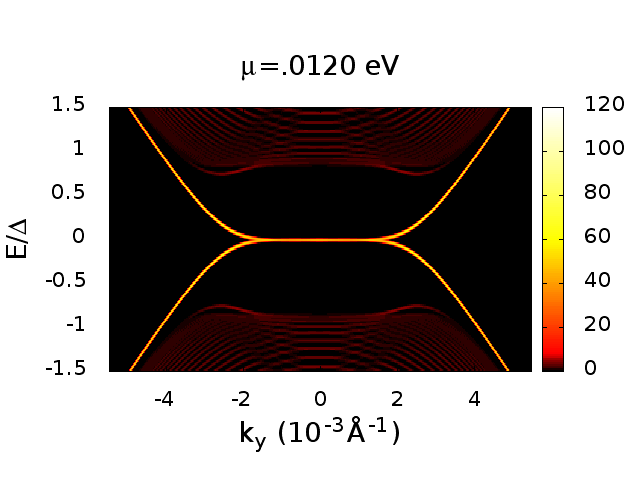
\includegraphics[width=.3\textwidth]{include/spectral/0120.png}
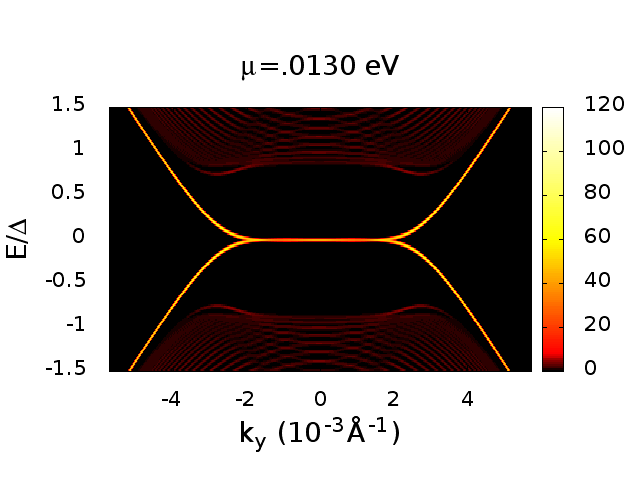
\includegraphics[width=.3\textwidth]{include/spectral/0130.png}
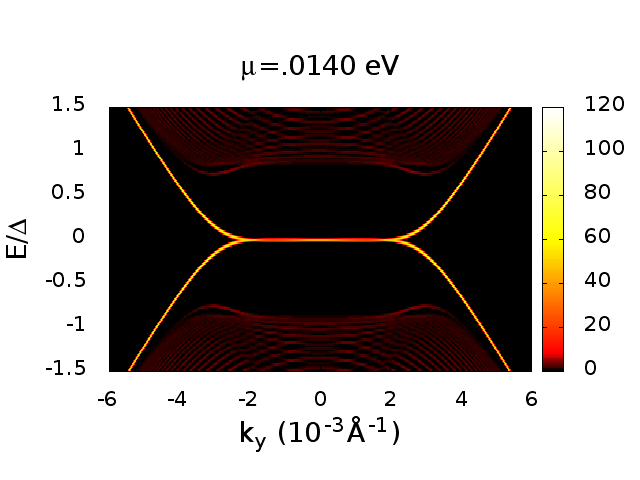
\includegraphics[width=.3\textwidth]{include/spectral/0140.png}\\

\caption{(color online) 
Spectral density function, $A(x=.5L,k_y,E)$, for values of $\mu$ from 0 eV to .14 eV. This images are used in a movie found online\cite{lababidimovie}. The linear dispersion ($E\sim k$) transitions to a flat band ($E\sim k^N$) as $\mu$ increases. This flat band is responsible for the peak in DOS in figure \ref{dosf}.
}\label{movie}
\end{figure}


\section{Periodic $\pi$ Junction}
Having established the existence of nearly flat ABS around zero energy, now
we systematically trace the evolution from the infinitesimal $\mu$, linear dispersing (Majorana) regime
to the large $\mu$ flat ABS regime. Also we would like to understand the details of ABS 
within its narrow ``band width". To this end, we will consider a simple model which generalizes the $\pi$ Josephson
junction to periodic systems. Namely, in Eq. (\ref{ham}), the order parameter modulates sinusoidally 
in the $x$-direction with period $2a$ as schematically shown in the upper panel of Fig. \ref{array}, 
\begin{equation}
\Delta(x)=\Delta  \sin(\pi x/a).
\end{equation}
The sign of the order parameter alternates. Thus the structure is effectively a periodic array of
the $\pi$ junctions discussed above in the limit $w \rightarrow 0$. One also recognizes that
$\Delta(x)$ describes a stripe or Larkin-Ovchinnikov superconductor \cite{LO}.
While such superconductors are hard to find, one may imagine bringing them in contact with a TI to realize
the model consider here. Now the Hamiltonian $\mathcal{H}$ has discrete
translational symmetry in the $x$-direction, $\mathcal{H}(x)=\mathcal{H}(x+2a)$. We can apply the 
Bloch-Floquet theorem and introduce quasi-momentum $k_x$ living in the Brillouin zone of $(-\pi/2a,\pi/2a)$. 
For the prescribed $\Delta(x)$, the energy spectrum $E(k_x,k_y)$
can be obtained by diagonalizing $\mathcal{H}$ in $k$-space. Note that the TI (non-superconducting) region is shrunk
to a point, only the homogeneous $\mu$ is left as tuning parameter.


\begin{figure}[h]
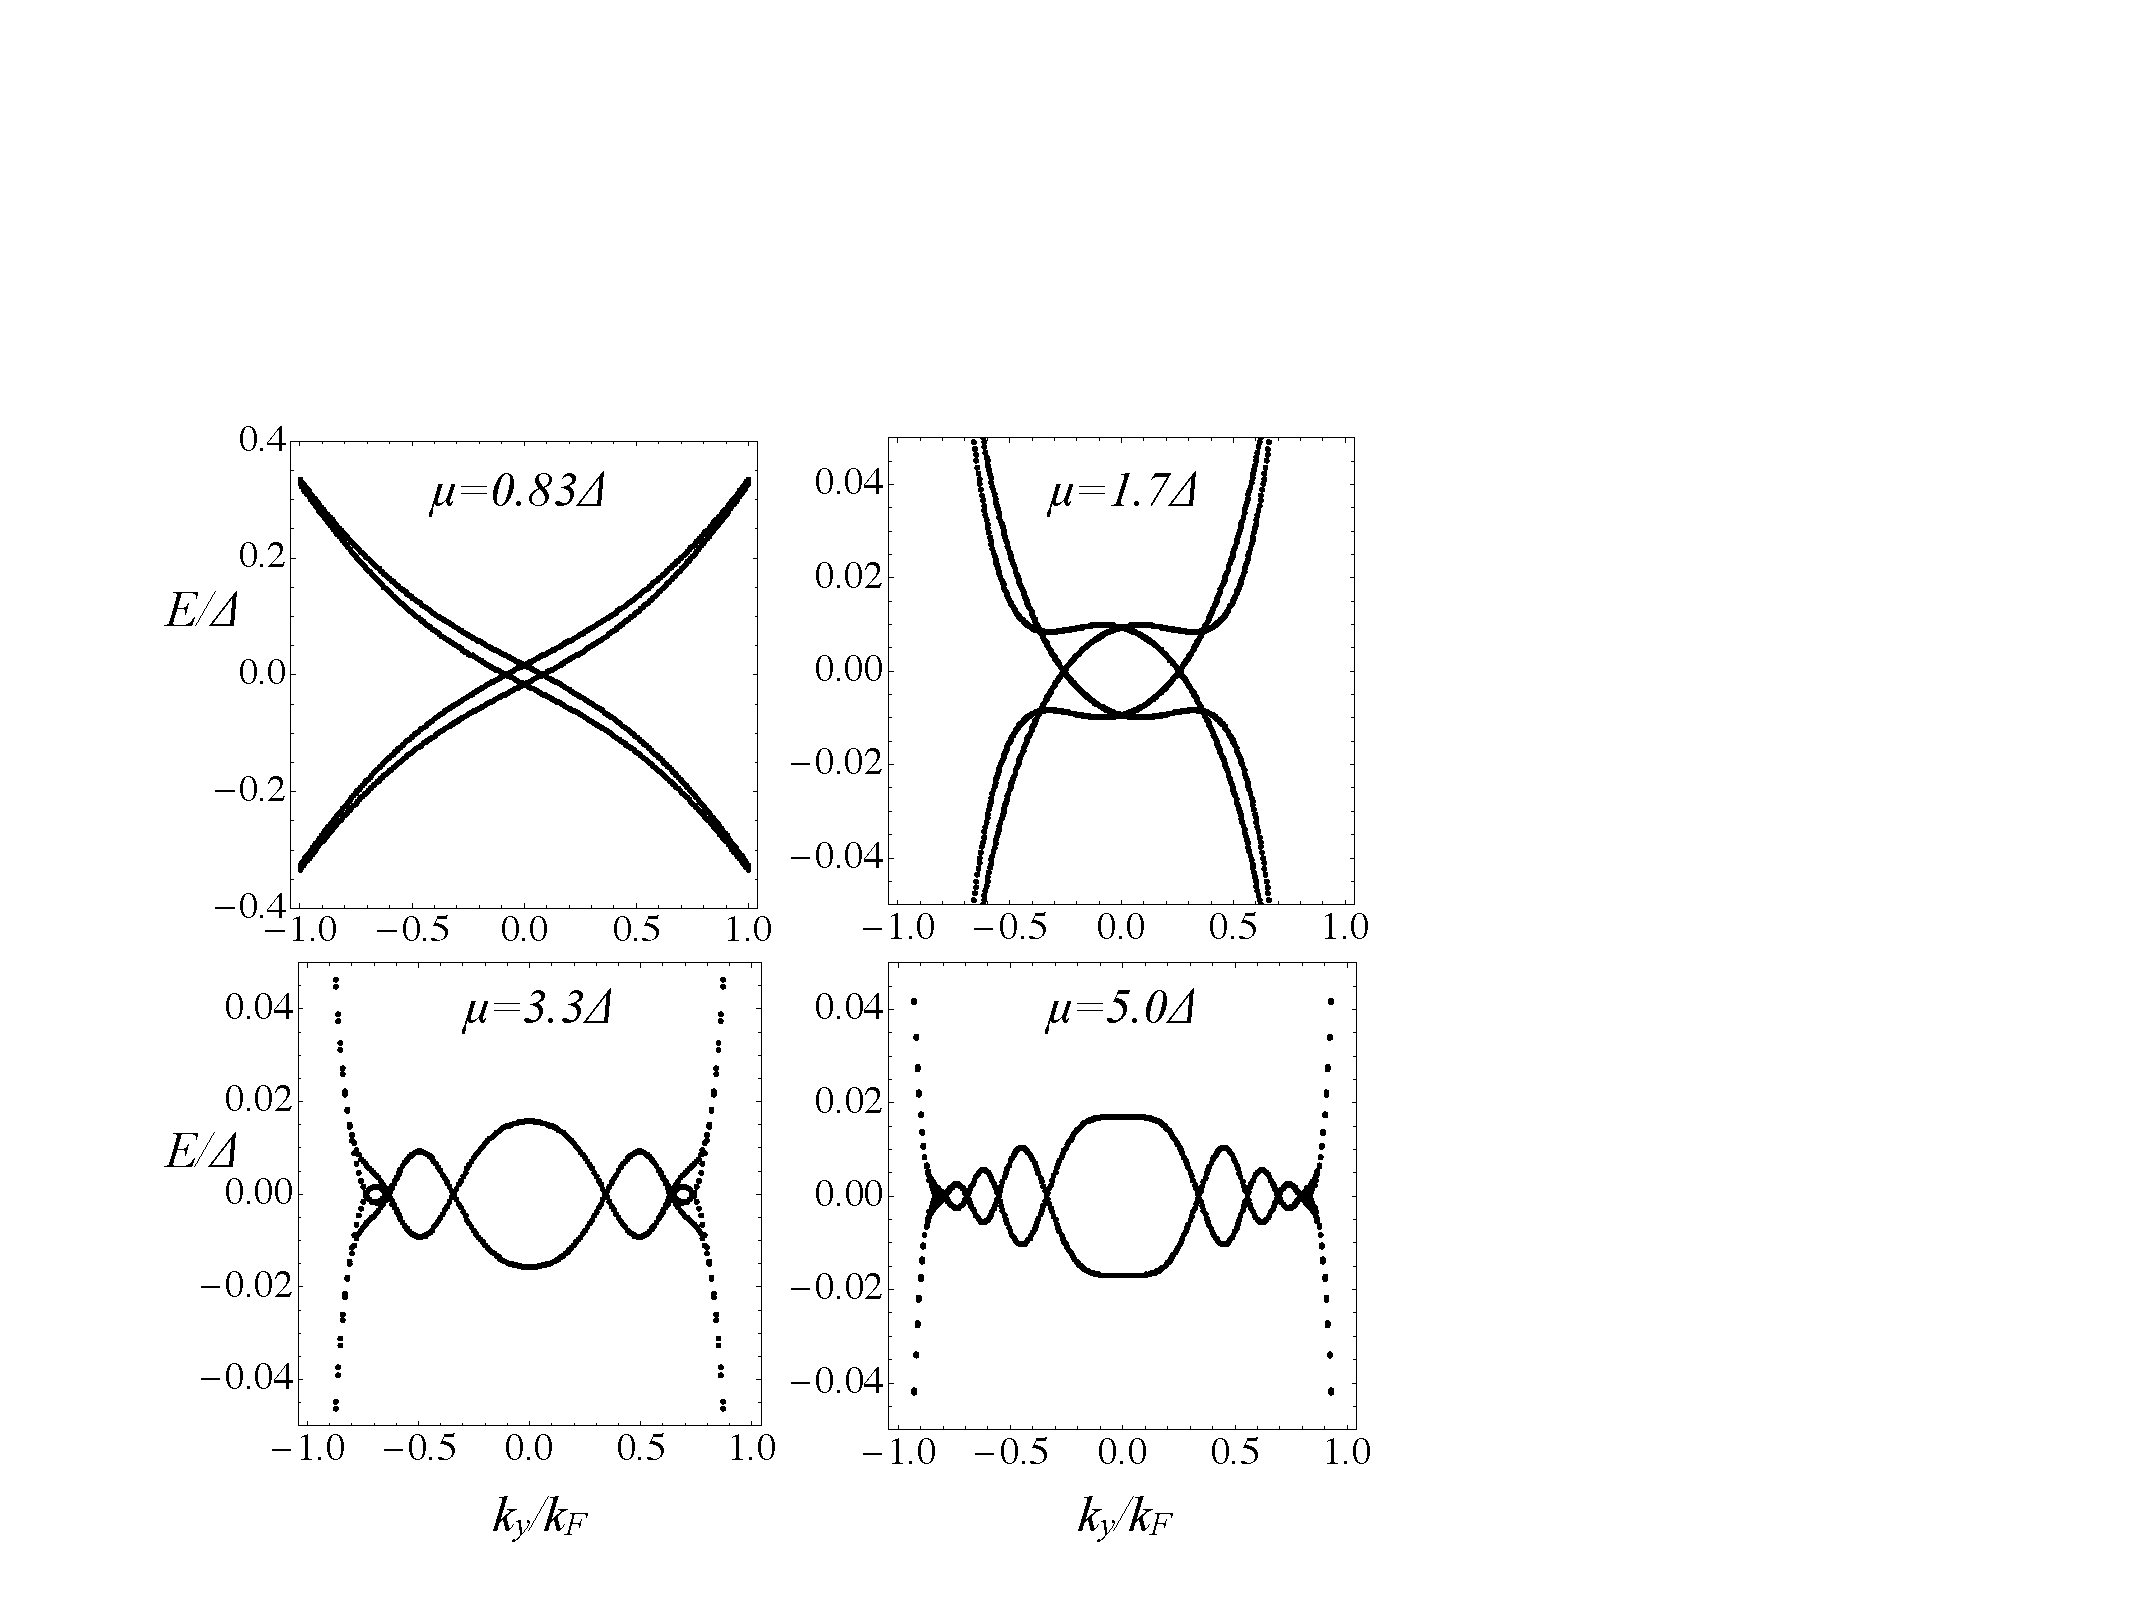
\includegraphics[width=\textwidth]{include/fig4.pdf}
\caption{Fine structures in the energy spectrum of the periodic proximity structure with fixed $a=12
\hbar v_F/\Delta$
and increasing $\mu$. The linearly dispersing Majorana spectrum at $\mu=0$ splits and develops
curvature to eventually become nearly flat within $(-k_F,k_F)$. The number of zero energy
crossings increases with $\mu$.
}\label{comp}
\end{figure}

The lower panel of Fig. \ref{array} shows the spectrum $E(k_x=0,k_y)$ for $a=24\hbar v_F/\Delta$, $\mu=4\Delta$. 
These flat ABS at zero energy do not show significant
variation with $k_x$. We have checked that the wave function of these zero energy states
are localized at the domain wall boundaries of the order parameter field, i.e., at $x=ma$ (red
curve in the upper panel of Fig. \ref{array}). For example, the wave function of the $k_y=0,k_x=0,E\approx 0$ 
mode can be fit well with periodic Gaussian functions $|u(x)|\propto \exp(-{1.85 (\pi x/\sqrt{2}a)^2})$.
Since $a$ is large in this case, these results agree well with the single junction result before.
The dispersion, for example, can be fit well using the ansatz in Eq. (\ref{bigN}).
The vanishing band width is, of course, only valid on coarse scales. Closer inspection, by blowing up the spectrum near zero as
illustrated in Fig. \ref{comp}, reveals the busy life of the ABS with $N_c$ crossings at zero energy,
where $N_c$ scales linearly with $\mu$, in agreement with Fig. \ref{jjsetup}d).
Remarkably, all these fine details are compressed within a small energy range. 

Fig. \ref{comp} illustrates the evolution of the ABS at low energies for the periodic structure
as $\mu$ is increased from zero. For small value of $\mu=0.83 \Delta$, the linear Majorana dispersion splits
into two, each developing a curvature, as
the zero energy crossings move to finite $k_y$ values. Further increasing $\mu$,
these two crossings are stretched further outward, while the dispersion within $k_y\in(-k_F,k_F)$ 
begin being bent and stretched to form the precursor of the flat band. At the same time,
addition of new crossings introduces more twists. The number of crossing scales with $N_c\sim \mu/\Delta$.
The spaghetti now becomes a rope, and looking from
afar, it appears as a thin thread.

\section{Summary}
Flat bands are more novelties than the norm in condensed matter \cite{heikkila_flat_2011}. Recently, several authors have
demonstrated that {\it surface} Andreev bound states with flat dispersion arise in certain topological 
superconductors, for example Cu$_x$Bi$_2$Se$_3$ \cite{hsieh_majorana_2012} and 
non-centrosymmetric superconductors \cite{PhysRevB.84.020501, schnyder_topological_2011}. 
Their existence can be traced
back to the nontrivial topology associated with the gapped bulk, and thus are topologically protected. 
This mechanism giving rise to flat bands, via the bulk-boundary correspondence,
differs from what is considered here. For example, in Ref. \cite{hsieh_majorana_2012},
a robust crossing at $k=0$ is a crucial point in the argument, and the total number of zero energy 
crossings is guaranteed an odd number. In our case, states at $k_y=0$ are gapped
for finite size systems (or finite period $2a$). Despite these differences, the
zero modes share the common trait that they are associated with the sign change of the order parameter
when electrons are reflected at the surface or interface.


Several groups have successfully fabricated Josephson structures on Bi$_2$Se$_3$ of various
length using a variety of 
superconducting materials including Al, Al/Ti, W, Nb, and Pb etc. \cite{SacACpAC:2011vn,
PhysRevB.84.165120,
Veldhorst:2012uq,Qu:2012kx,2012arXiv1202.2323W}. 
Gate tunable supercurrent
has been observed and argued to be due to the TI surface state \cite{SacACpAC:2011vn}. Superconducting quantum 
interference devices based on such junctions have also been demonstrated \cite{2011arXiv1112.5858V,Qu:2012kx}. 
Thus the flat
Andreev bound states at zero energy, and the zero bias conductance peak in the local 
density of states, predicted here should be experimentally accessible. 
Future work will explore control of these slowly dispersing Andreev levels
working as qubits \cite{PhysRevLett.90.087003}
when confinement in the $y$ direction is also introduced. Our work
also suggests the ac dynamics of the S-TI-S junctions will likely to be very complex
featuring different regimes.
The flat ABS at zero energy predicted for periodic junction arrays may potentially find 
technological applications. For example, a diverging density of states at the midgap
may be used to generate microwave resonances.

We would like to thank Noah Bray-Ali, Liang Fu, and Takuya Kitagawa for helpful discussions.






\chapter{Summary and Outlook}

Thus far, we have delved into the physics of heterostructures of superconductors and topological insulators, starting with the TI's interaction with a metal and ending with a Josephson junction on the surface of the TI. 

We found that electrons traveling from the metal to the surface of the TI can have a perfect spin flip under certain conditions. 
In addition we found that there occurs a hybridization between the metal and the surface of the TI, where the spectrum near the surface of the TI resembles that of the metal when the metal is strongly in contact with the TI. 
One possibility to extend the spin-flip mechanism found would be to have two surfaces of TIs sandwiching a metal. This flat 2D quantum device could have implications in spintronics applications.

In the study of the heterostructure of a superconductor and TI, we found that there does exist a subgap mode that penetrates deep into the superconductor. The parameters that describe this mode are renormalized from the respective bulk values of the individual materials due to the interplay between the TI and superconductor. A serious possibility on continuing this focus of microscopic simulation of a S-TI heterostructure is by simulating, more realistically, a Weyl superconductor, a periodic array of S-TI heterostructures with magnetic doping on the TI segments. The Weyl superconductor is an exotic gapless superconductor\cite{meng_weyl_2012}. This prospective direction has experimental implications due to experimental realizations in magnetically doped TIs\cite{liu_magnetic_2009,chen_massive_2010,zhang_topology-driven_2013}. 

The Josephson junction on the surface of the TI gives rise to some very unique phenomena. The energy spectrum shows that when the junction's phase is $\pi$, the linear energy dispersion morphs into a flat, zero-slope dispersion as the chemical potential is tuned away from zero. This dispersion also presents a strong peak in the density of states. 
The progression from this study has a few directions. The flat band, illustrates that the quasiparticle excitations have ``low" kinetic energy and therefore secondary interactions, if they can be induced, can lead to new phases. And lastly, the ground state of the junction can be determined by comparing the free energy for different phase biases. This realistic study could precipitate further experiments to find the zero-energy Majorana mode.


\appendix
\vspace{0in}
\chapter{Additional Papers}
\pagestyle{empty}
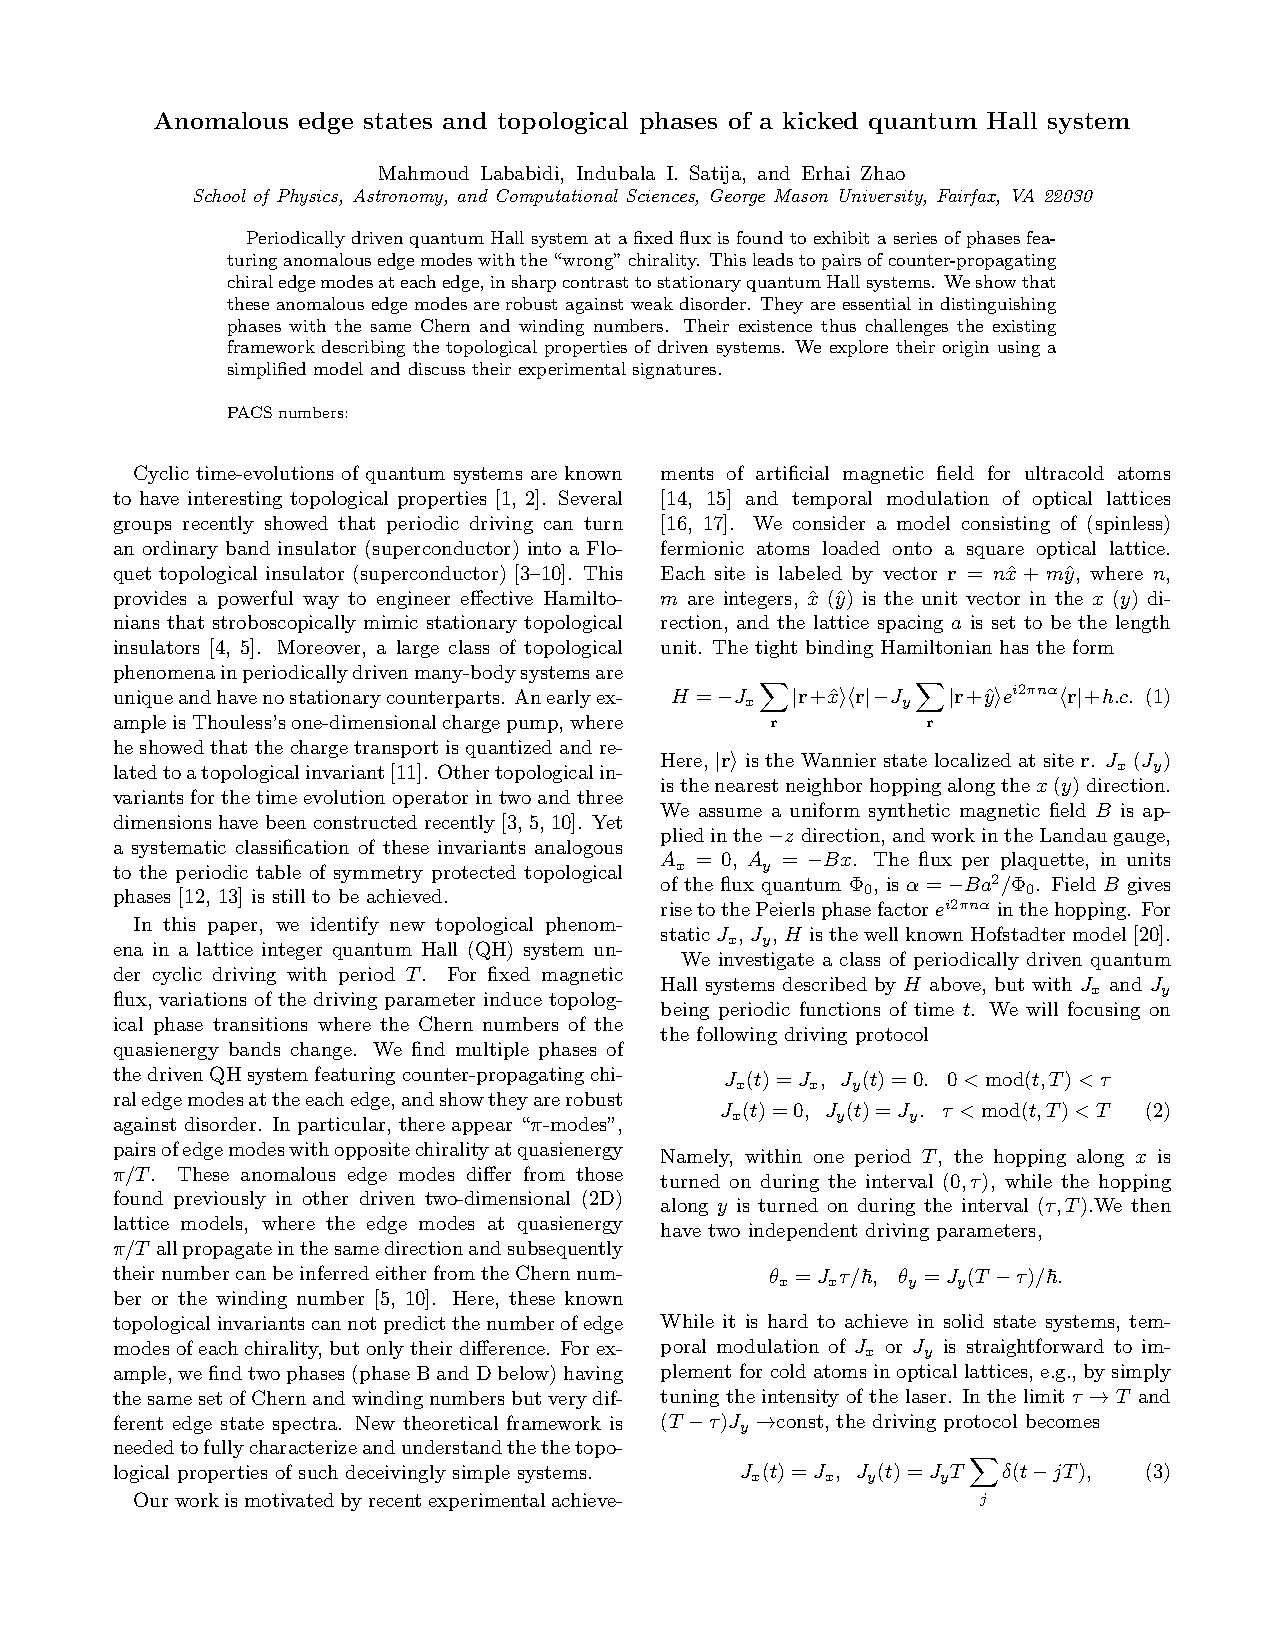
\includepdf[pages={-},fitpaper=true, offset=.25in -.5in,pagecommand=\thispagestyle{plain},noautoscale=true,scale=.85]{chap/kicked.pdf}
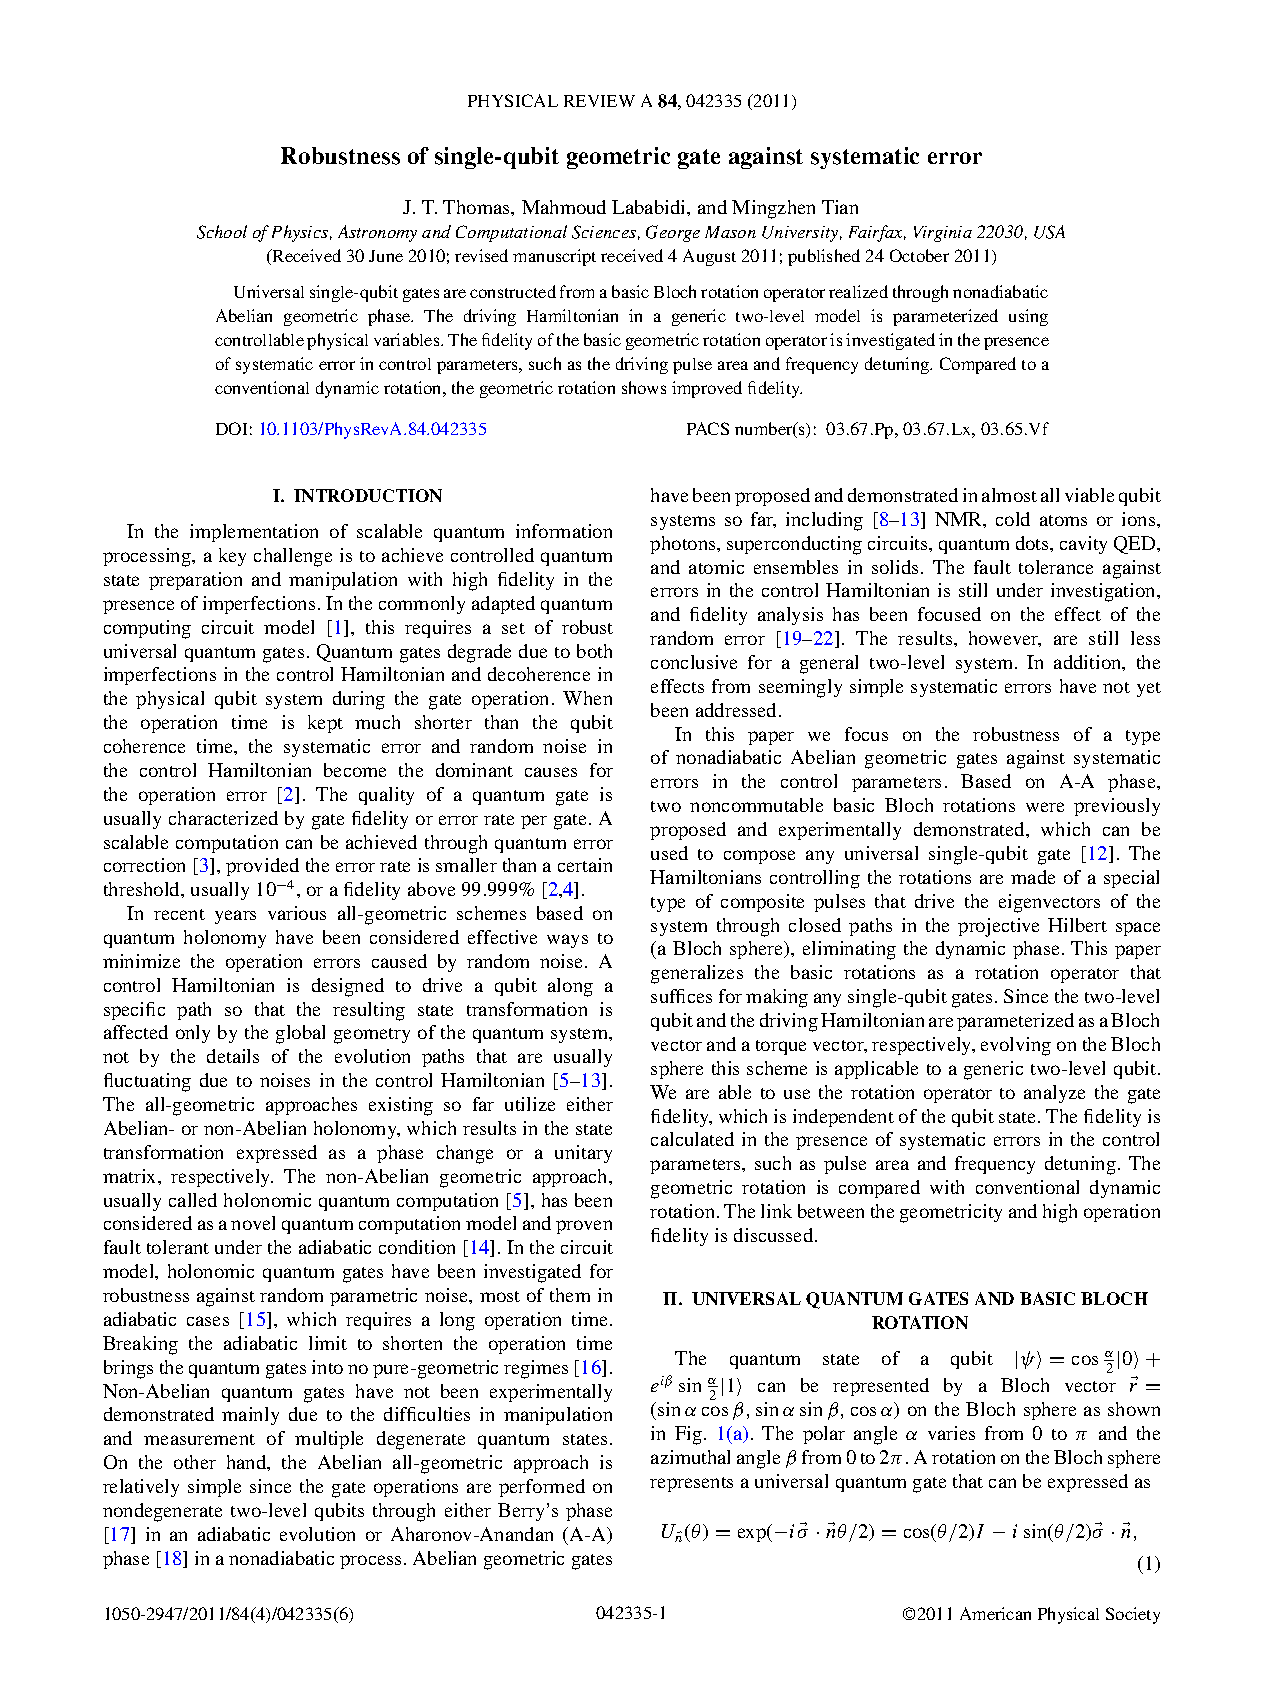
\includepdf[pages={-},fitpaper=true, offset=.25in -.5in,pagecommand=\thispagestyle{plain},noautoscale=true,scale=.85]{chap/pra.pdf}

% A first, optional argument in [ ] is the title as displayed in the table of contents
% The second argument is the title as displayed here.  Use \\ as appropriate in
%   this title to get desired line breaks


\bibliographystyle{aip}
\bibliography{dissertation,prox,intro}{}

\cvpage

\noindent Mahmoud Lababidi was born in 1983 in the United States. He earned his Bachelor of Science in Computer Engineering from the University of Florida, Gainesville in 2006. He enrolled in the Physics PhD program at George Mason University in 2008 and began working under the supervision of Professor Erhai Zhao in 2010. 

\vspace{1em}
\noindent List of Publications
\begin{description}
\item[I] \hfill\\
Mott scattering at the interface between a metal and a topological insulator\\
Erhai Zhao and Chun Zhang and Mahmoud Lababidi\\
Physical Review B 82, 205331
\item[II] \hfill \\
Microscopic simulation of superconductor/topological insulator proximity structures\\
Mahmoud Lababidi and Erhai Zhao\\
Physical Review B 83, 184511
\item[III] \hfill\\
Nearly flat Andreev bound states in superconductor-topological insulator hybrid structures\\
Mahmoud Lababidi and Erhai Zhao\\
Physical Review B 86, 161108(R)
\item[IV] \hfill\\
Anomalous edge states and topological phases of a kicked quantum Hall system\\
Mahmoud Lababidi, Indubala I. Satija, and Erhai Zhao\\
arXiv:1307.3569
\item[V] \hfill\\
Robustness of single-qubit geometric gate against systematic error\\
J. T. Thomas, Mahmoud Lababidi, and Mingzhen Tian\\
Physical Review A 84, 042335
\end{description}


\end{document}
